\documentclass[a4paper,12pt]{article}\usepackage[]{graphicx}\usepackage[]{color}
%% maxwidth is the original width if it is less than linewidth
%% otherwise use linewidth (to make sure the graphics do not exceed the margin)
\makeatletter
\def\maxwidth{ %
  \ifdim\Gin@nat@width>\linewidth
    \linewidth
  \else
    \Gin@nat@width
  \fi
}
\makeatother

\definecolor{fgcolor}{rgb}{0.345, 0.345, 0.345}
\newcommand{\hlnum}[1]{\textcolor[rgb]{0.686,0.059,0.569}{#1}}%
\newcommand{\hlstr}[1]{\textcolor[rgb]{0.192,0.494,0.8}{#1}}%
\newcommand{\hlcom}[1]{\textcolor[rgb]{0.678,0.584,0.686}{\textit{#1}}}%
\newcommand{\hlopt}[1]{\textcolor[rgb]{0,0,0}{#1}}%
\newcommand{\hlstd}[1]{\textcolor[rgb]{0.345,0.345,0.345}{#1}}%
\newcommand{\hlkwa}[1]{\textcolor[rgb]{0.161,0.373,0.58}{\textbf{#1}}}%
\newcommand{\hlkwb}[1]{\textcolor[rgb]{0.69,0.353,0.396}{#1}}%
\newcommand{\hlkwc}[1]{\textcolor[rgb]{0.333,0.667,0.333}{#1}}%
\newcommand{\hlkwd}[1]{\textcolor[rgb]{0.737,0.353,0.396}{\textbf{#1}}}%
\let\hlipl\hlkwb

\usepackage{framed}
\makeatletter
\newenvironment{kframe}{%
 \def\at@end@of@kframe{}%
 \ifinner\ifhmode%
  \def\at@end@of@kframe{\end{minipage}}%
  \begin{minipage}{\columnwidth}%
 \fi\fi%
 \def\FrameCommand##1{\hskip\@totalleftmargin \hskip-\fboxsep
 \colorbox{shadecolor}{##1}\hskip-\fboxsep
     % There is no \\@totalrightmargin, so:
     \hskip-\linewidth \hskip-\@totalleftmargin \hskip\columnwidth}%
 \MakeFramed {\advance\hsize-\width
   \@totalleftmargin\z@ \linewidth\hsize
   \@setminipage}}%
 {\par\unskip\endMakeFramed%
 \at@end@of@kframe}
\makeatother

\definecolor{shadecolor}{rgb}{.97, .97, .97}
\definecolor{messagecolor}{rgb}{0, 0, 0}
\definecolor{warningcolor}{rgb}{1, 0, 1}
\definecolor{errorcolor}{rgb}{1, 0, 0}
\newenvironment{knitrout}{}{} % an empty environment to be redefined in TeX

\usepackage{alltt}
\usepackage[margin=1in]{geometry}
\usepackage[utf8]{inputenc}
%\usepackage{times}
\usepackage{booktabs}
\usepackage{multirow}
\usepackage{natbib}
\usepackage{amsmath}
\usepackage{setspace}
\usepackage[normalem]{ulem}
\usepackage{sectsty}
\subsectionfont{\normalfont\large\underline}
\usepackage{floatrow}
\floatsetup[figure]{capposition=top}
\floatsetup[table]{capposition=top}

\title{Measuring Subgroup Preferences in Conjoint Experiments}
\author{Thomas J. Leeper, Sara B. Hobolt, and James Tilley}
\IfFileExists{upquote.sty}{\usepackage{upquote}}{}
\begin{document}

\maketitle

{\abstract Conjoint analysis is an increasingly prominent tool for studying political preferences. The method powerfully disentangles patterns in respondents' favorability toward complex, multidimensional objects, such as political candidates or public policies. Most conjoint analyses rely upon a fully randomized conjoint design to generate average marginal component effects (AMCEs), which measure the degree to which a given value of a conjoint profile feature increases or decreases respondents' support for the overall profile relative to a baseline, averaging across all respondents and all other profile features. While the AMCE has a clear causal interpretation, most published conjoint analyses also use AMCEs to simply describe preferences, often including comparisons of AMCEs between subgroups of respondents. We show how this descriptive use of conditional AMCEs can be substantially misleading about the degree of agreement or disagreement between subgroups due the simple, but often forgotten, property that interactions are sensitive to the reference category used in regression analysis. This leads to inferences about subgroup differences in preferences that have arbitrary sign, size, and significance. We demonstrate the problem using examples drawn from the published literature and provide suggestions for improved reporting and interpretation using two quantities of interest: the marginal mean and the omnibus F-test. Given the rapidly accelerating use of conjoint analyses, this paper makes an important contribution by highlighting pitfalls and presenting advice for best practice in the analysis and presentation of conjoint experiments.}

















\clearpage


Amidst the dramatically increased use of experiments within political science \citep{Druckmanetal2006, Mutz2011}, conjoint experimental designs have recently become a prominent methodological tool in political science. While traditional survey experiments tend to examine just one or two factors that might shape outcomes \citep[see, for reviews,][]{GainesKuklinskiQuirk2007, Sniderman2011}, conjoint designs allow researchers to study the independent effects on preferences of many features of complex, multidimensional objects such as political candidates \citep{Campbelletal2016, TeeleKallaRosenbluth2018}, immigrant admissions \citep{HainmuellerHopkins2015, BansakHainmuellerHangartner2016, WrightLevyCitrin2016}, or public policies \citep{GallegoMarx2017, Hankinson2018}. The driving force behind this use of conjoint analysis has been the introduction by \citet{HainmuellerHopkinsYamamoto2014} of a fully randomized conjoint design and an associated analytic approach that emphasizes a single quantity of interest: namely, the average marginal component effect (AMCE). By capturing the multidimensionality of target objects, the randomized conjoint design breaks any explicit or implicit confounding between features of these objects, giving the AMCE a clear causal interpretation: the degree to which a given value of a feature increases or decreases respondents' favorability toward a packaged conjoint profile relative to a baseline, averaging across all respondents and all other profile features. 

While randomization of profile features gives the AMCE a causal interpretation, most published conjoint analyses in political science use AMCEs for \textit{descriptive} purposes: that is, to map variation in favorability toward a multidimensional object across its various features. This is particularly the case when researchers engage in subgroup analyses of conjoint experiments in search of preference heterogeneity. For example, \citet{HainmuellerHopkinsYamamoto2014} perform a subgroup analysis on their original immigration experiment in which they perform a median split on a measure of ethnocentrism and then compare AMCEs for the two subgroups. Similarly, \citet{BansakHainmuellerHangartner2016} compare preferences toward immigrants across number of binary respondent characteristics: age, education, left-right ideology, and income. In a different domain, \citet{BallardRosaMartinScheve2016} compare preferences over tax policies across a number of subgroups defined by demographics and political orientations. \citet{TeeleKallaRosenbluth2018} compare AMCEs for features of male and female political candidates among male and female respondents. \citet{KirklandCoppock2017} do a similar comparison between Democrats and Republicans in hypothetical elections.

In these and many other articles, interpretation of these subgroup analyses focus not just on the \textit{causal effects} of profile features within each subgroup (what Hainmueller et al. term ``conditional AMCEs''; 13) but also on an implied quantity of interest: the \textit{difference} between two conditional AMCEs across subgroups. Searching for causal effect heterogeneity is an increasingly common feature of experimental analysis \citep{GreenKern2012, RatkovicTingley2017, GrimmerMessingWestwood2017}, yet most conjoint analyses use this difference-in-AMCEs instead to \textit{descriptively} interpret apparent differences in favorability toward objects with a given feature (e.g., immigrants from Syria) between the two groups (e.g., low and high ethnocentrism respondents).

What is not necessarily obvious in such analyses is that differences-in-preferences (that is to say, the difference in degree of favorability toward profiles containing a given feature) are not directly reflected in differences-in-AMCEs. Yet authors frequently use visual or more formal comparisons of conditional AMCEs to make descriptive claims about such differences, leading themselves and readers astray. Differences in AMCEs do not provide inference into difference between subgroups' favorability toward a conjoint feature. In this paper, we show that a difference in underlying subgroup preferences --- like a difference in willingness to support a Syrian immigrant between high and low ethnocentrism respondents --- is only reflected in the difference-in-AMCEs under particular preference configurations and analytic choices. The underlying cause of this error is simple and familiar to any applied researcher but appears to be forgotten in most applied conjoint work.

As we will show, where preferences in subgroups toward the experimental reference category are similar, the difference-in-AMCEs conveys preferences reasonably well but where preferences between subgroups diverge in the reference category, the difference-in-AMCEs is a misleading representation of underlying patterns of favorability. Yet most published conjoint studies appear to report results based upon reference categories chosen for \textit{substantive} reasons about the nature or meaning of the levels rather than the configuration of preferences revealed in the experiment. Ultimately AMCEs are relative, not absolute, statements about preferences so subgroup differences are also relative not absolute statements about preference heterogeneity.\footnote{For example, in a comparison of subgroup effects for Democrats and Republicans, Republicans might display a smaller effect because their preferences in the reference category are already very positive, such that a large positive effect for Democrats occurs despite Democrats being less supportive than Republicans in either experimental condition.} There is simply no predictable inference to be drawn from subgroup causal effects to the levels of underlying subgroup opinion. This inferential error --- interpreting differences in the size of causal effects as descriptive differences in preferences --- appears to be widespread in published conjoint analyses. The root of this error is likely familiar to many researchers: it is simply a matter of regression specification for models involving interactions between categorical regressors. \citet{EgamiImai2018}, for example, provide an extensive discussion of the implications of this property for interpreting causal interactions between features of conjoint profiles. The state of the published literature would suggest the problem remains non-obvious when applied to descriptive analysis of subgroups in conjoint designs.

In what follows, we demonstrate the challenges of conjoint analysis and reminder readers of how reference category choice for profile features creates significant problems for comparing conditional AMCEs across respondent subgroups. We show how the use of an arbitrary reference category means the size and the direction of differences-in-AMCEs have little relationship to the underlying degree of favorability of the subgroups toward profiles with particular features and that reference category choices can make similar preferences look dissimilar and dissimilar preferences look similar, using examples drawn from the published political science literature (namely experiments by \citealt{HainmuellerHopkinsYamamoto2014, BallardRosaMartinScheve2016, TeeleKallaRosenbluth2018}). The paper then provides suggestions for improved conjoint reporting and interpretation based around two quantities of interest drawn from the factorial experimentation literature: (1) unadjusted marginal means, a quantity measuring favorability toward a given feature, and (b) an omnibus F-test, measuring differences therein. Newly developed software for the R programming language to support our findings --- and that can be used to examine sensitivity of conjoint analysis to reference category selection, calculate AMCEs and marginal means, perform subgroup analyses, and test for subgroup differences in any conjoint experiment --- is demonstrated throughout. We conclude with advice for best practices in the analysis and presentation of conjoint results.

\section*{Quantities of Interest in Conjoint Experiments}\label{sec:quantities}

Conjoint analysis serves two purposes. One is to assess causal effects. Another is preference description.\footnote{Here we use ``preference'' as \citet{HainmuellerHopkinsYamamoto2014} do: that is, as a statement of \textit{favorability} or \textit{support} for a profile, not the more narrow economic definition of a strict rank ordering of objects by favorability.} In causal inference, conjoints provide a design and analytic approach that allows researchers to understand the causal effect of a given feature on overall support for a multidimensional object, averaging across other features of the object included in the design. Such inferences can be thought of as statements of the form: ``shifting an immigrant's country of origin from India to Poland increases favorability by X percentage points.'' In descriptive inference, conjoints provide information about both (a) the \textit{absolute} favorability of respondents toward objects with particular features or combinations of features, and (b) the \textit{relative} favorability of respondents toward an object with alternative combinations of features. Such inferences can be thought of as statements of the form ``Polish immigrants are preferred by X\% of respondents'' or ``Polish immigrants are more supported than Mexican immigrants, by X percentage points.'' Thus both causal and descriptive interpretations of conjoints are based upon the distribution of preferences across profile features and differences in preferences across alternative feature combinations.

Importantly, a fully randomized conjoint design without constraints between profile features is simply a full-factorial experiment (with some cells possibly, albeit randomly, left unobserved). All quantities of interest relevant to the analysis of conjoint designs derive from combinations of cell means, marginal means, and the grand mean, as is common in the traditional analysis of factorial experiments. In a forced choice design, the \textit{grand mean} is by definition 0.5 (i.e., 50\% of all profiles shown are chosen and 50\% are not chosen). \textit{Cell means} are the mean outcome for each particular combination of feature levels. In the full-factorial design discussed by \citet{HainmuellerHopkinsYamamoto2014} and now widely used in political science, many or perhaps most cell means are unobserved. For example, in their candidate choice experiment, there are $2*6*6*6*2*6*6*6 = 186,624$ cell means but only 3,466 observations so about 98\% of cell means are unobserved. While this would be problematic for attempting to infer pairwise comparisons between cells, conjoint analysts mostly focus on the marginal effects of each feature rather than more complex interactions. Appendix \ref{app:quantities} provides detailed notation and elaborations of these definitions of quantities of interest.

Average marginal component effects (AMCEs) depend only upon \textit{marginal means}: that is the column and row mean outcomes for each feature level averaging across all other features. A marginal mean describes the level of favorability toward profiles that have a particular feature level, marginalizing across all other features. For example, in the common forced-choice design with two alternatives, marginal means have a direct interpretation as probabilities: a marginal mean of 0 indicates respondents select profiles with that feature level with probability $Pr(Y=1|X=x) = 0$ while a marginal mean of 1 indicates respondents select profiles with that feature level with probability $(Pr(Y=1|X=x)=1$.\footnote{It is not possible for the marginal mean to equal zero or one if pairs of profiles shown together are allowed to have the same level of a given feature (for example, both immigrants are from Germany). Instead, the marginal mean can range from the probability of co-occurrence to 1 minus that probability. If there are five levels of a feature, each shown with equal probability, then the probability of co-occurrence is $\frac{1}{5}*\frac{1}{5} = 0.04$ such that the marginal mean can take values in the range $(0.04,0.96)$. If the design is constrained so that features cannot be the same for both immigrants, then the marginal means fully range from zero to one. This constraint on the range of the marginal means also constrains the range of AMCEs. Notably, many conjoints provide features with only two levels, such as the male-versus-female candidate feature examined by \citet{TeeleKallaRosenbluth2018}. In such cases, the probability of co-occurrence is $\frac{1}{2}*\frac{1}{2} = 0.25$ bounding the AMCE for female (as opposed to male) candidates to the range $(-0.5, 0.5)$ if both candidates can have the same sex. Caution is therefore needed in comparing the relative size of features with few levels to features with many levels given that effects have different bounds.} With rating scale outcomes, marginal means can vary arbitrarily along the outcome scale used.

\begin{knitrout}
\definecolor{shadecolor}{rgb}{0.969, 0.969, 0.969}\color{fgcolor}\begin{figure}
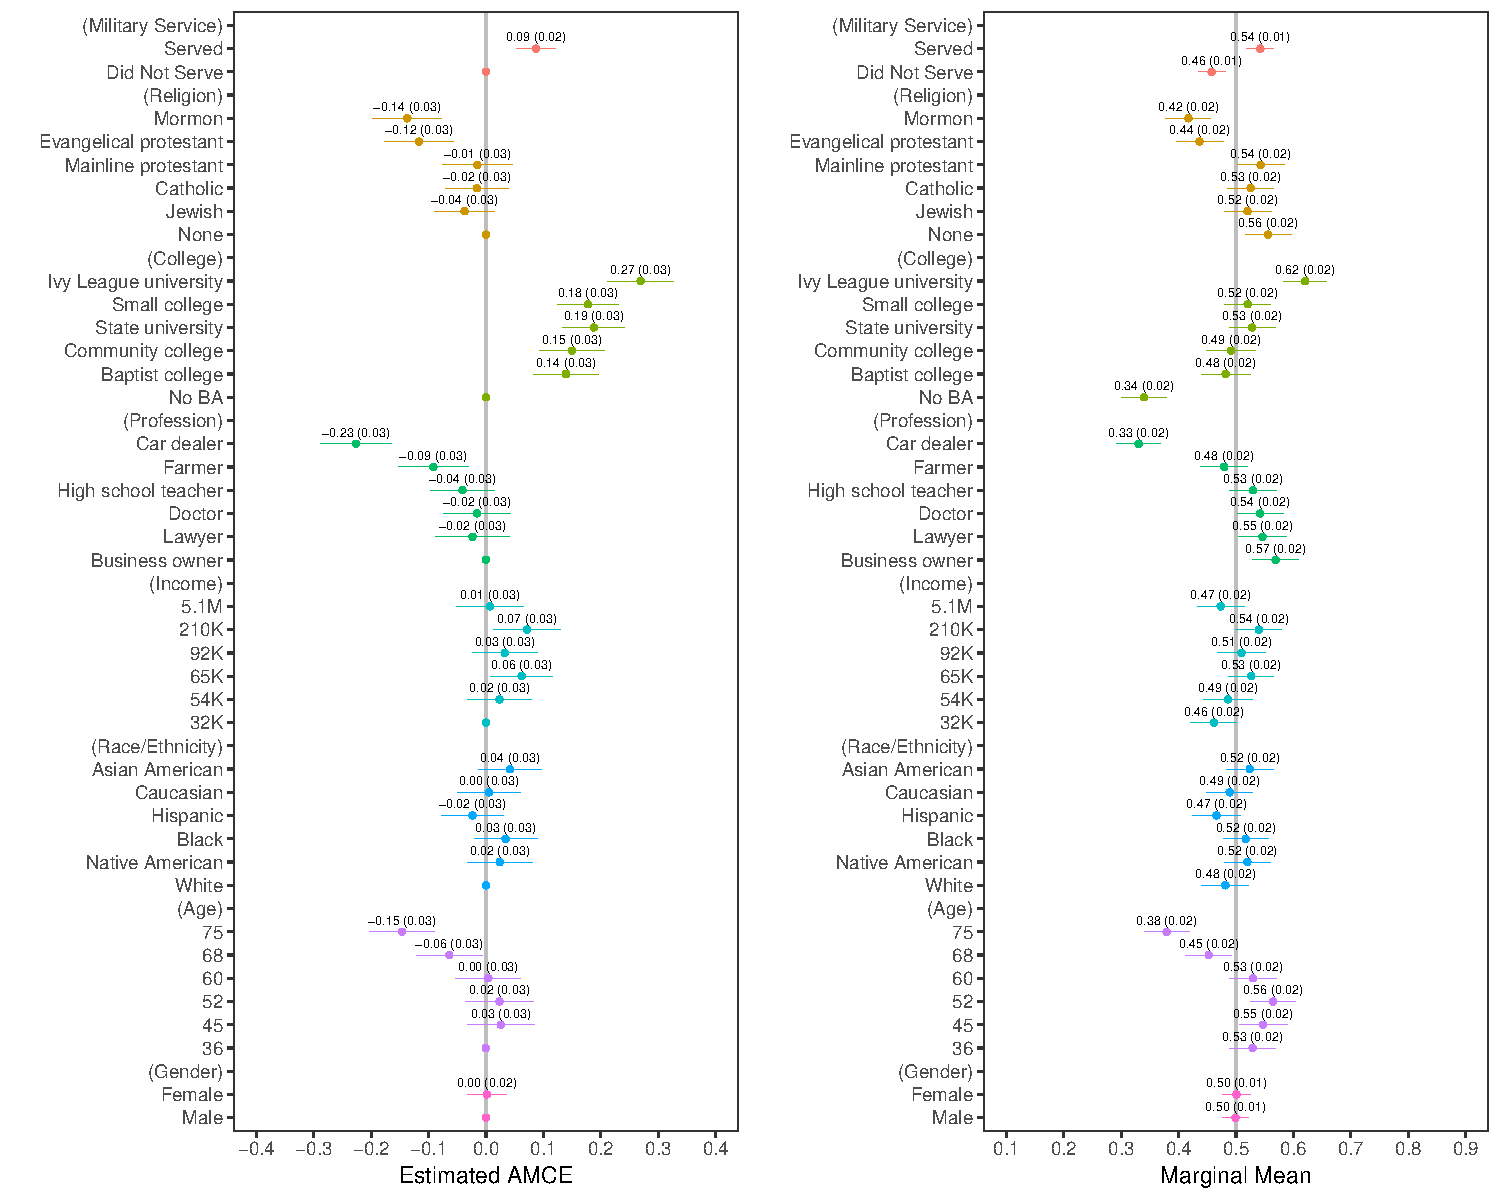
\includegraphics[width=\maxwidth]{figure/hainmueller_candidate_replication-1} 
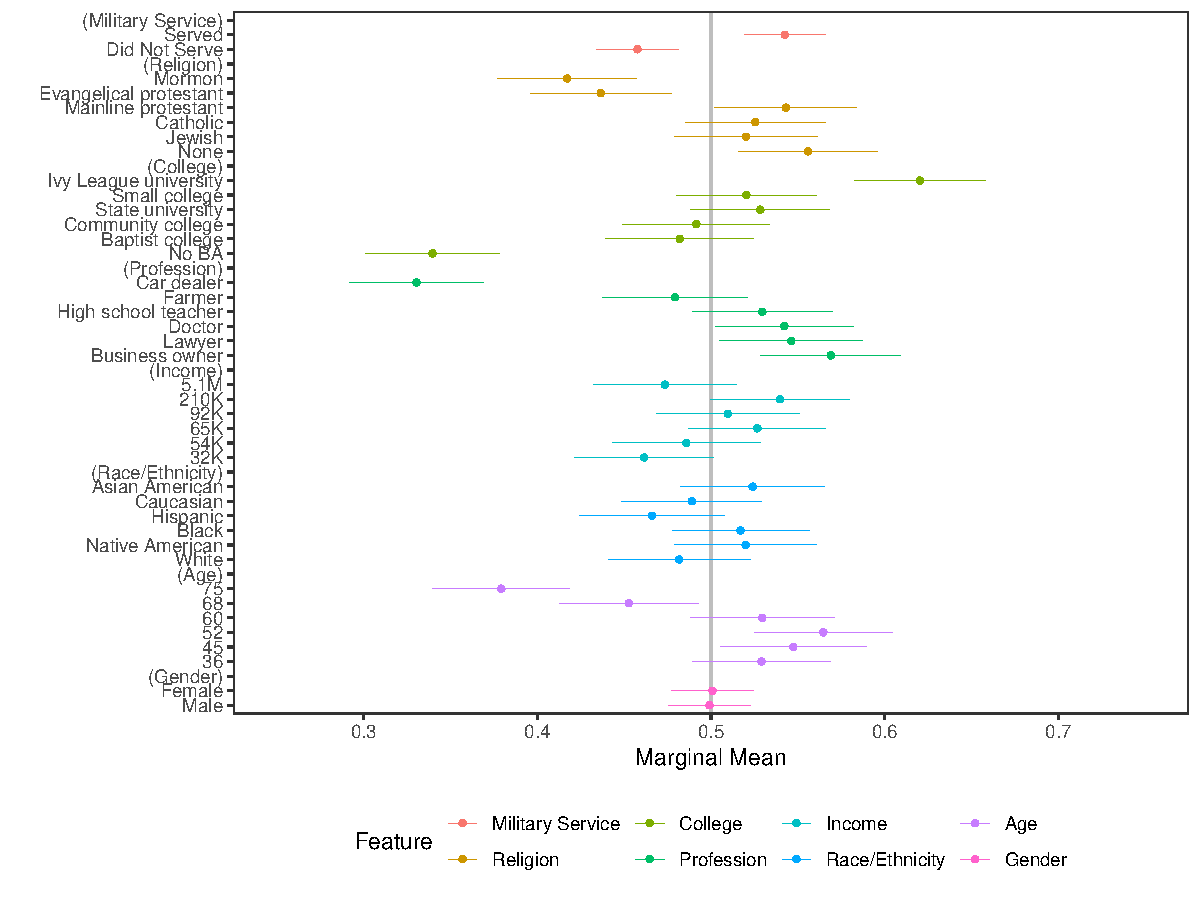
\includegraphics[width=\maxwidth]{figure/hainmueller_candidate_replication-2} \caption[Replication of Hainmueller et al]{Replication of Hainmueller et al. (2014) Candidate Experiment using AMCEs and MMs}\label{fig:hainmueller_candidate_replication}
\end{figure}


\end{knitrout}

Because levels of features are randomly assigned, pairwise differences between two marginal means for a given feature (e.g., between candidates who are male versus female) have a direct causal interpretation. For fully randomized designs, the AMCE proposed by \citet{HainmuellerHopkinsYamamoto2014} is equivalent to the average marginal effect of each feature level for a model where each feature is converted into a matrix of indicator variables with one level left out as a reference category. This is no different from any other regression context wherein one level of any categorical variable must be omitted from the design matrix in order to avoid perfect multicollinearity.\footnote{In designs that entail constraints between profile features, the average marginal effect is a weighted average of effects across each combination of the constrained features where the weights on the effects are arbitrary but typically uniform. We ignore this distinction in the remainder of this article, as all of our results apply equally to fully randomized and to constrained designs.} This close relationship between AMCEs and marginal means is visible in Figure \ref{fig:hainmueller_candidate_replication} which presents a replication of the AMCE-based analysis of the Hainmueller et al. candidate experiment (upper panel) and an analogous examination of the results using marginal means (lower panel). Here and throughout we use visual presentation of results, but full numerical estimates including appropriate standard errors are presented in the Appendix. Note, in particular, how marginal means convey information about the preferences of respondents for all feature levels while AMCEs definitionally restrict the AMCE for the reference category to zero (or undefined). For example, the AMCE for a candidate serving in the military is 0.09 (or a 9-percentage point) increase in favorability, reflecting marginal means for serving and non-serving candidates of 0.46 and 0.54, respectively.

The AMCE is often described as an estimate of the relative favorability of profiles with counterfactual levels of a feature; for example, ``male candidates are preferred to female candidates'' \citep[6]{TeeleKallaRosenbluth2018}. \citet{HainmuellerHopkinsYamamoto2014} similarly describe some of the results of conjoint on preferences toward Congressional candidates:

\begin{quote}
We also see a bias against Mormon candidates, whose estimated level of support is 0.06 (SE = 0.03) lower when compared to a baseline candidate with no stated religion. Support for Evangelical Protestants is also 0.04 percentage points lower (SE = 0.02) than the baseline. (19)
\end{quote}

\noindent These examples make clear that despite the \textit{causal} inference potentially provided by the AMCE, the quantity of interest is frequently used to provide a characterization of a preferences that has a distinctly descriptive flavor. Indeed, this style of description is widespread in conjoint analyses. \citet{BallardRosaMartinScheve2016} interpretation their tax preference conjoint:

\begin{quote}
we find strong support for progressive preferences over federal income taxes among the American public [\dots] respondents are less likely to support a given tax plan as the tax rate on the poorest three groups increases but more likely to support an income tax policy when the tax rate on the richest two groups increases, at least to a point.
\end{quote}

\noindent This use of conjoints to provide descriptive inferences about patterns of preferences is important because AMCEs are defined as \textit{relative} quantities, requiring that patterns of preferences are expressed against a baseline, reference category for each conjoint feature. A positive (negative) AMCE is read as higher (lower) favorability but it is only higher (lower) relative to whatever category serves as the baseline. For example, in the \citeauthor{HainmuellerHopkinsYamamoto2014} candidate example, choosing a non-religious candidate as a baseline means the AMCEs in the candidate experiment are all expressed relative to this non-religious baseline; the difference (if any) between other pairs of marginal means (e.g., evaluations of Mormon and Evangelical candidates) is not obvious. Relatedly, the negative direction (and the size) of the AMCEs for Mormon and Evangelical candidates would be different if the least-liked category (Mormon candidates) were the reference group. In that case, the AMCE for Evangelicals would be small and positive and the AMCEs for all other categories (including the presented reference category, ``none'') would be large and positive.

\begin{knitrout}
\definecolor{shadecolor}{rgb}{0.969, 0.969, 0.969}\color{fgcolor}\begin{figure}
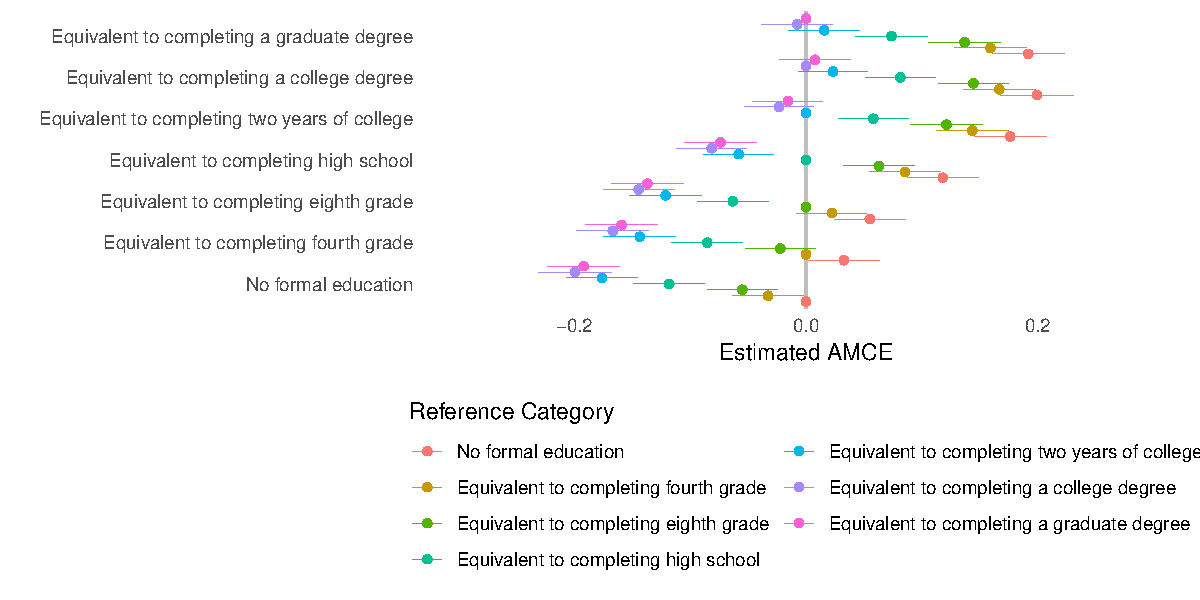
\includegraphics[width=\maxwidth]{figure/reference_category-1} \caption[Reference Category Diagnostic for the 'Education' Feature from Hainmueller et al.'s (2014) Immigration Experiment]{Reference Category Diagnostic for the 'Education' Feature from Hainmueller et al.'s (2014) Immigration Experiment}\label{fig:reference_category}
\end{figure}


\end{knitrout}

Being a familiar analytic problem in any regression context, this choice of reference category for estimating AMCEs can seem trivial but is quite consequential. For example, in \citeauthor{HainmuellerHopkinsYamamoto2014}'s candidate experiment, the least liked education level (``no formal education'') is chosen as a reference category, but the authors could have presented the results using any of the categories as the baseline. Figure \ref{fig:reference_category} shows how the estimated AMCEs for each level of education would have differed depending on that choice. Selecting a reference category that receives middling support (i.e., more favorability than some other feature levels but less favorability than others), makes some AMCEs positive and others negative but all AMCEs can be made positive (or negative) simply by choosing a different baseline.\footnote{As another example, in \citeauthor{BallardRosaMartinScheve2016}'s tax preference experiment, the lowest level of taxation is chosen as the reference category for each feature for reasons of substantive interpretation, yet despite the substantive intuitiveness of this, favorability toward the lowest level of taxation is not necessarily higher or lower than preferences for alternative tax rates.} The results would be numerically equivalent --- the alternative linear models used to the estimate the AMCEs have a mathematical equivalence --- but the choice has sizeable consequences for the interpretation of conjoint analyses, as we discuss below.\footnote{In \textit{constrained} conjoint designs, the choice of reference category is even more important. Consider, for example, the design of \citeauthor{HainmuellerHopkinsYamamoto2014}'s immigration experiment, which constrains the ``Country of Origin`` feature so that levels `India,' `Germany,' `France,' `Mexico,' `Philippines,' and `Poland' cannot co-occur with the `Escape Persecution' level of the ``Reason for Application'' feature. Consequently, the AMCE for the ``Escape Persecution'' level (relative to the  ``Reunite with family'' reference category) is only defined for the subset of the design involving countries `China,' `Sudan,' `Somalia,' and `Iraq.' The AMCEs for those four countries (relative to India as a baseline) marginalize across all reasons for application, but the AMCEs for the first six countries marginalize only across the latter two reasons. Thus the interpretation of AMCEs --- and the basic ability to estimate them in constrained designs --- depends entirely upon the selection of a reference category where all feature levels can co-occur. In a design where \textit{all} features are constrained, then AMCEs are undefined for the design as a whole and only estimable for subsets of the design that are \textit{conditionally} unconstrained.}

%To demonstrate this, Figure \ref{fig:reference_category} shows the estimated AMCEs for the country of origin feature from \citeauthor{HainmuellerHopkinsYamamoto2014}'s immigration experiment, with the analysis repeated ten times each time using a different country as the reference category. For example, the top-most set of points and error bars convey the AMCE for Iraq from each of these analyses. When Iraq is the reference category, its AMCE is undefined. When any other country is chosen as a reference category, the AMCE for Iraq is negative because respondents are more negative toward Iraqi immigrants than they are toward those of other countries. Similarly, the bottom set of points and error bars reflects the estimated AMCEs for Germany. When Germany is the reference category, its AMCE is undefined but when any other country is used as the reference category, its AMCE is positive.

%These cases are therefore not \textit{directionally} sensitive to the choice of reference category but of course the point estimates vary considerably. But the estimated AMCE of countries who are neither strongly disliked or strongly favored by respondents are highly sensitive to choice of reference category. Consider, for example, the estimated AMCEs for China (the four set of points from the top). When highly disliked countries are chosen as the reference category (like Somalia, Sudan, or Iraq), the AMCE for China is positive; when highly favored countries are chosen (like Germany, Poland, or the Philippines), the AMCE for China is negative.

\section*{Consequences of Arbitrary Reference Category Choice}\label{sec:challenges}

Given the need to choose a reference category for every feature in order to estimate AMCEs, an important question is: how do researchers decide which of tens of thousands of possible experimental cells should be selected as the reference category? Examining recently published conjoint analyses, it appears that the choice of reference category is either arbitrary or based upon substantive intuition about the meaning of feature levels. For example, \citet{HainmuellerHopkinsYamamoto2014} choose female immigrants as a baseline in their immigration experiment, thus providing an estimate of the AMCE of being male, while \citet{TeeleKallaRosenbluth2018} choose male candidates as a baseline in their conjoint, thus providing an estimate of the AMCE of being female. The choice is seemingly innocuous. Sometimes choices of reference category appear to be driven by substantive knowledge: on language skills of immigrants, \citet{HainmuellerHopkinsYamamoto2014} choose fluency as a baseline; on the prior trips to the US feature, ``never'' is chosen as the baseline. These seem sensible on face value --- it might seem less useful to define all effects relative to ``having visited many times as a tourist'' as the AMCEs then lose an immediately intuitive interpretation.

% Difference in conditional AMCEs
\begin{table}
\caption{Uses of Subgroup Analysis Published in Political Science Journals}\label{tab:papers}
\begin{center}
\footnotesize
\begin{tabular}{p{2in} p{2in} p{2in}}\toprule
\textbf{Paper} & \textbf{Topic} & \textbf{Subgroup Comparisons} \\ \midrule
\citet{BechtelScheve2013} & Climate agreement preferences & Environmentalism and International Reciprocity Attitudes \\ \midrule
\citet{FranchinoZucchini2014} & Candidate preferences & Political Interest, Left-right self-placement\\ \midrule
\citet{HainmuellerHopkinsYamamoto2014} & Immigration preferences & Ethnocentrism \\ \midrule
\citet{HansenOlsenBech2014} & Policy preferences & Partisanship \\ \midrule
\citet{Carlson2015} & Candidate preferences & Co-ethnicity \\ \midrule
\citet{BansakHainmuellerHangartner2016} & Immigration preferences & Left-right self-placement, age, education, income\\ \midrule
\citet{BallardRosaMartinScheve2016} & Tax preferences & Various\\ \midrule
\citet{Campbelletal2016} & Candidate preferences & Partisanship \\ \midrule
\citet{CarnesLupu2016} & Candidate preferences & Partisanship \\ \midrule
\citet{Mummolo2016} & News selection & Various\\ \midrule
\citet{VivyanWagner2016} & Candidate preferences & Political attitudes \\ \midrule
\citet{MummoloNall2017} & Mobility preferences & Partisanship \\ \midrule
\citet{BechtelGenoveseScheve2017} & Climate agreement preferences & Employment sector emissions \\ \midrule
\citet{BechtelHainmuellerMargalit2017} & International bailout preferences & Various\\ \midrule
\citet{GallegoMarx2017} & Labor market policy & Left-right self-placement \\ \midrule
\citet{KirklandCoppock2017} & Candidate preferences & Partisanship \\ \midrule
\citet{Sen2017} & Judicial candidate preferences & Partisanship \\ \midrule
\citet{Sobolewskaetal2017} & Immigrant integration & Various \\ \midrule
\citet{EggersVivyanWagner2018} & Candidate preferences & Sex \\ \midrule
\citet{Hankinson2018} & Housing policy preferences & Various \\ \midrule
\citet{OliverosSchuster2018} & Bureaucrat candidate preferences & Various \\ \midrule
\citet{TeeleKallaRosenbluth2018} & Candidate preferences & Sex, Partisanship \\ \midrule
\citet{Careyetal2018} & Hiring preferences & Various \\ \midrule
\bottomrule
\end{tabular}
\end{center}
All articles in this table use subgroup conditional AMCEs to make inferences about differences in preferences between subgroups.
\end{table}

Yet the choice is consequential. A possibly surprising consequence of the seemingly arbitrary selection of a reference category --- and the resulting arbitrariness of both the size and direction of AMCEs --- is that it can provide highly distorted descriptive interpretation of preferences among subgroups of respondents. This occurs when researchers examine \textit{conditional} AMCEs, wherein AMCEs are calculated separately for subgroups of respondents and those conditional estimates are directly compared \citep[13]{HainmuellerHopkinsYamamoto2014}. Table \ref{tab:papers} reports a list of recently published articles in political science that engage in this form of subgroup analysis.\footnote{\citet{RatkovicTingley2017} considered efficient methods for performing subgroup analyses in conjoint designs. Our focus here is on the narrower problem of interpreting subgroup analyses as traditionally performed using subsetting or interaction terms in a regression framework.} Given the commonly descriptive interpretations of conjoint experimental results, such subgroup analyses seem perfectly intuitive and the set of subgroups listed in the last column of Table \ref{tab:papers} contains some unsurprising covariates, such as partisanship, that are of obvious theoretical interest in almost any study of individual preferences. Analytically, these conditional AMCEs can be obtained either from regression estimates on respondent subgroups or through interactions between conjoint features and respondent characteristics, the details of which are unimportant for our purposes.

Conditional AMCEs are not per se a problematic quantity of inference. Like subgroup analysis of any experiment, they convey the causal effect of an experimental factor on overall favorability among the subgroup of interest. Consider, for example, a two-condition party cue experiment where Democrats and Republicans are exposed to an endorsement cue from the Democratic party or no cue and opinions toward the policy serve as the outcome. It is sensible to imagine that effects of the cue might differ for the two groups and therefore to compare the size of cue effect among the two groups. Perhaps Democrats are more responsive to the Democratic party cue than are Republicans, making the causal effect larger for Democrats than Republicans. Discussions of conditional AMCEs in conjoint analyses often explicitly or implicitly engage in this kind of discussion comparing the size and direction of subgroup causal effects. If interpreted as a difference in the size of the causal effect for two groups, such comparisons are perfectly consistent with more traditional experimental analysis and a perfectly acceptable interpretation of the conjoint results.

\begin{knitrout}
\definecolor{shadecolor}{rgb}{0.969, 0.969, 0.969}\color{fgcolor}\begin{figure}
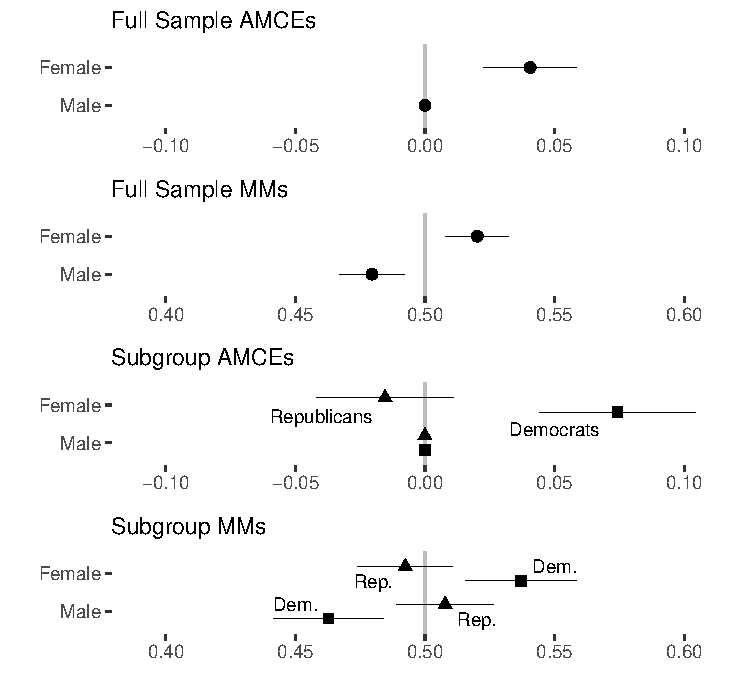
\includegraphics[width=\maxwidth]{figure/tkr_replication-1} 
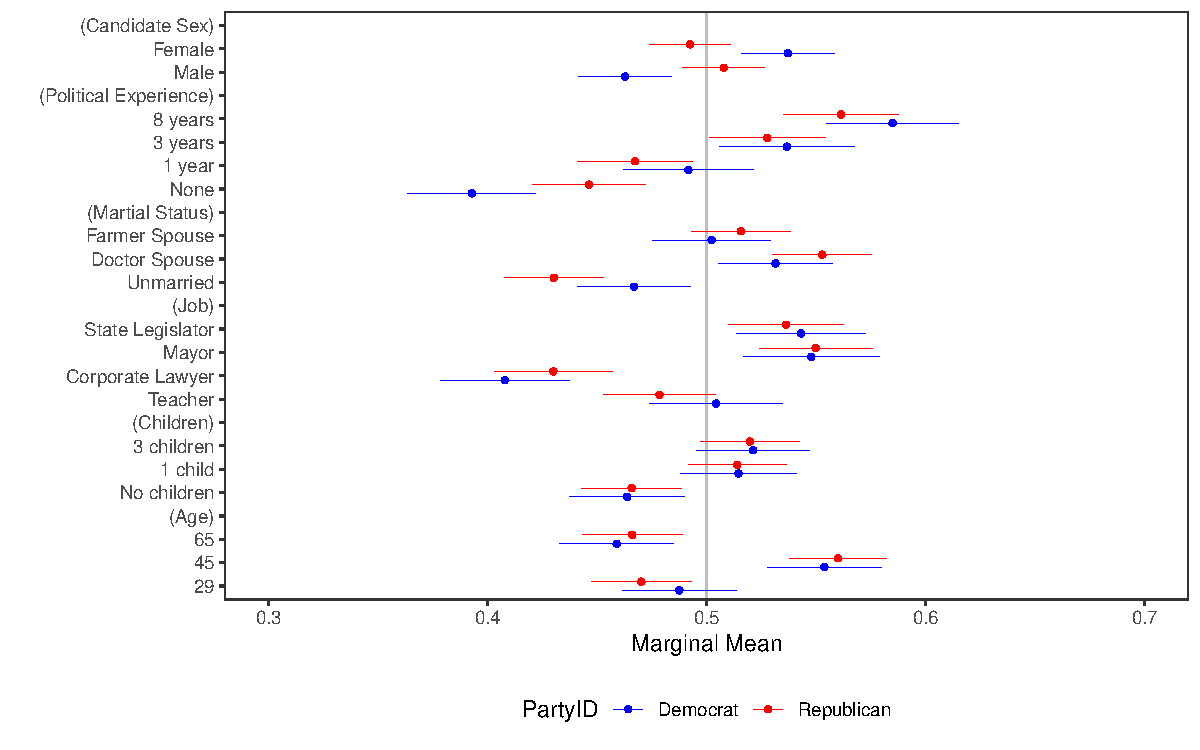
\includegraphics[width=\maxwidth]{figure/tkr_replication-2} \caption[Replication of Teele et al]{Replication of Teele et al. (2018) Candidate Experiment using AMCEs and MMs}\label{fig:tkr_replication}
\end{figure}


\end{knitrout}

Yet, just as analysis of full sample conjoint data is often descriptive in nature, so too do conjoint analysts frequently interpret differences in conditional AMCEs descriptively rather than causally. For example, in one analysis \citet{HainmuellerHopkinsYamamoto2014} visually compare the pattern of AMCEs among high- and low-ethnocentrism respondents and interpret that ``the patterns of support are generally similar for respondents irrespective of their level of ethnocentrism'' (22). \citet{BallardRosaMartinScheve2016} make similar comparisons in their tax policy conjoint: ``While there are few strong differences in preferences for taxing the lower three income groups (the `hard work' group has slightly lower elasticities for taxing the poor), there are strong differences in preferences for taxing the rich. Respondents who believe luck plays a role in economic success are more strongly progressive, although preferences over taxing the \$175K--\$375K bracket are relatively flat'' (12). In these examples, the differences between conditional AMCEs are used as a way of descriptively characterizing differences in \textit{preferences} between the groups rather than differences in \textit{causal effects on preferences} in the groups.

As a more complete example, the upper panel of Figure \ref{fig:tkr_replication} shows AMCEs for \citeauthor{TeeleKallaRosenbluth2018}'s candidate choice experiment separately for Democratic and Republican voters, as provided in the original paper, and the lower panel shows the results using conditional marginal means. Again, we opt for visual presentation of results; tabular presentation of AMCEs, marginal means, and associated standard errors for all examples are included in the Appendix. Respondents' preference for female candidates is very apparent in both forms of analysis. Yet the discrepancy between the differences in preferences (i.e., conditional marginal means) and the differences in conditional AMCEs can be seen very clearly in the ``political experience'' feature in Figure \ref{fig:tkr_replication} (the second set of estimates from the top in both panels). The conditional AMCEs in the upper panel correctly convey that both Democrats and Republicans are more likely to favor experienced than inexperienced candidates. Reading the AMCEs descriptively, however, would suggest that Democratic voters are more favorable toward candidates with all levels of experience compared to Republican voters (i.e., Republicans and Democrats differ in their preferences over experienced candidates). In reality, however, the conditional marginal means shown in the lower panel demonstrate that actually Democrats and Republicans have very similar preferences toward candidates with 1 or 3 years of experience, but differ dramatically in their preferences over candidates with no experience (the reference category) and those with 8 years experience. Democrats are much more sensitive to experience than are Republicans and important differences in preferences are apparent for extreme categories in the visualization of conditional marginal means, but the conditional AMCEs suggest that preferences differ at all levels of experience, when in reality they do not. The selection of a reference category is therefore hugely consequential for a descriptive reading of the AMCE results.

Interpreting conjoint AMCEs as measures of preferences is an inferential error. In a simple experiment like the party cue example just given, this kind of interpretation would be obviously flawed. A larger causal effect of the party cue for Democrats than Republicans does not necessarily mean that Democrats are more supportive than Republicans on average or in either condition. Effects are relative, not absolute, statements about preferences. Republicans, for example, might experience a smaller effect because their preferences in the control group are already very supportive, such that a large positive effect for Democrats occurs despite Democrats being less supportive than Republicans in either experimental condition. There is simply no predictable connection between subgroup causal effects and the levels of underlying subgroup preferences. This inferential error --- interpreting differences in the size of causal effects as descriptive differences in preferences --- appears to be widespread in published conjoint analyses. While AMCEs do provide insight into the descriptive variation in preferences within-group and across-features, and conditional AMCEs do estimate the size of causal effects of features within groups, AMCEs cannot provide direct insight into the pattern of preferences between groups because they do not provide information about \textit{absolute} levels of favorability toward profiles with each feature (or combination of features).

This additional information matters. Consider again the simple two-condition experiment in which the effect of a cue treatment, $x \in {0,1}$, is compared across a single two-category covariate, $z \in {0,1}$ such as Democratic or Republican self-identification. Subgroup regression equations to estimate effects for each group are:

\begin{align*}
\hat{y} &= \beta_0 + \beta_1 x, \quad \forall z = 0 \\
\hat{y} &= \beta_2 + \beta_3 x, \quad \forall z = 1
\end{align*}

\noindent The effect of $x$ when $z=0$ is given by $\beta_1$. The effect of $x$ when $z=1$ is given by $\beta_3$. These are, in essence, the conditional AMCEs in a conjoint analysis. Yet the difference in AMCEs ($\beta_3 - \beta_1$) is not equal to the difference in preferences between the two groups, which is $\bar{y}_{z=1|x=1} - \bar{y}_{z=0|x=1}$ (estimated by $(\beta_2 + \beta_3) - (\beta_0 + \beta_1)$). The difference-in-AMCEs only equals the difference in preferences when $\beta_2 \equiv \beta_0$. Yet the standard AMCE-centric conjoint analysis does not present or characterize either of these quantities. Similarity of conditional AMCEs therefore only convey similarity of the \textit{causal effect} of the feature, but do not convey similarity of \textit{preferences} unless preferences toward profiles with the reference category are equivalent across groups. Given the reference category choice is typically arbitrary or driven by substantive knowledge of the levels, there is never any reason to expect that an arbitrarily selected reference category satisfies that equality assumption. When using a difference-in-AMCEs comparison to estimate a difference in preferences, the size and direction of the bias is determined by the size of the difference in preferences toward the reference category within each subgroup.

\begin{knitrout}
\definecolor{shadecolor}{rgb}{0.969, 0.969, 0.969}\color{fgcolor}\begin{figure}
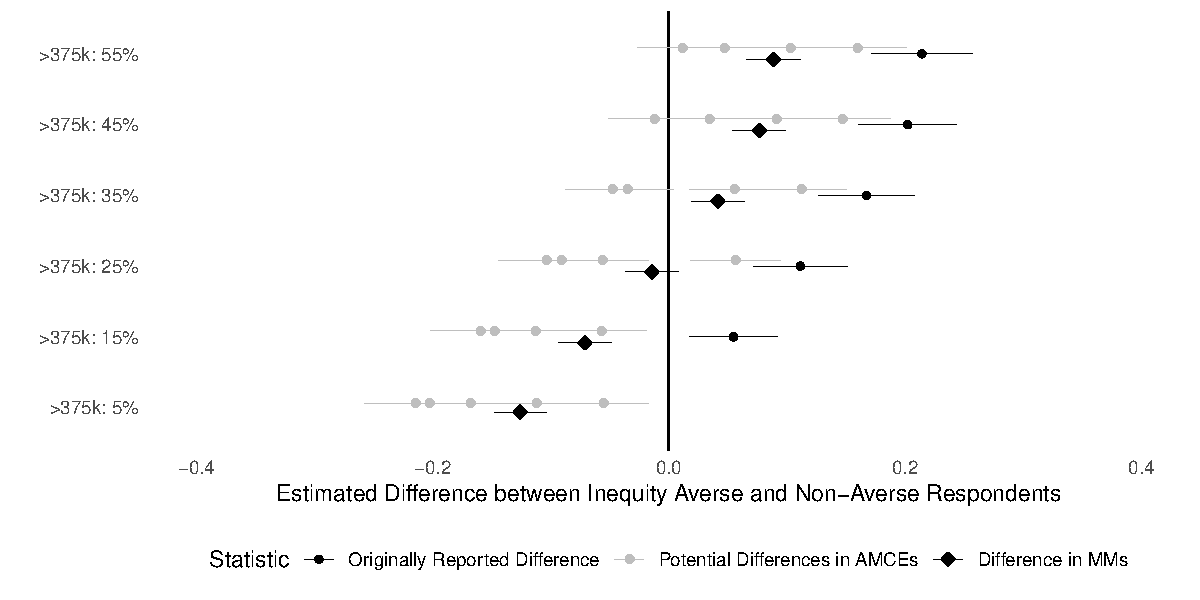
\includegraphics[width=\maxwidth]{figure/bms_difference_comparison-1} \caption[Estimated Preference Differences between Inequity Averse and Non-Averse Respondents from Ballard-Rosa et al]{Estimated Preference Differences between Inequity Averse and Non-Averse Respondents from Ballard-Rosa et al. (2016) Tax Preference Experiment for Each Possible Reference Category}\label{fig:bms_difference_comparison}
\end{figure}


\end{knitrout}

We can see this bias clearly in a reanalysis of \citeauthor{BallardRosaMartinScheve2016}'s tax preference experiment. Figure \ref{fig:bms_difference_comparison} shows an analysis for the feature capturing the tax rate for the highest earners (those over \$375,000 per year) replicating a portion of the results they present comparing inequity averse and non-averse respondents \citet[9 figure 2]{BallardRosaMartinScheve2016}. The original analysis was presented as conditional AMCEs for the two subgroups with inequity averse respondents having positive AMCEs for all tax levels (relative to 5\% as the reference category) and AMCEs for non-averse respondents being largely indistinguishable from zero. Figure \ref{fig:bms_difference_comparison} presents the implied difference-in-AMCEs from the original analysis as round black dots, demonstrating the substantial and positive \textit{apparent} differences between the two groups. The black diamonds show the true differences in marginal means between the two groups. The gray dots represent the alternative differences-in-AMCEs that could have been generated from alternative choices of reference category using the same data. Because respondents in the two groups actually have substantially different preferences over the reference category 5\% tax rate (inequity averse respondents are much less favorable toward this rate than non-averse respondents) differences-in-AMCEs make it seem like inequity averse respondents are much \textit{more} favorable toward 15\% and 25\% tax rates than non-averse respondents, when in actuality averse respondents are \textit{less} favorable toward the 15\% tax rate than non-averse respondents and the two groups have largely similar views of a 25\% tax rate. Not only does the difference-in-AMCEs overestimate group differences for very high tax rates (35\%, 45\%, 55\%) but the difference-in-AMCEs flips the true direction of group differences for lower rates. The authors correctly read their data as showing ``support for more progressive preferences is correlated with concern over societal inequality'' \citep[9]{BallardRosaMartinScheve2016} but for the wrong reason: inequity averse and non-averse respondents are similarly favorable toward middling tax rates and diverge in their views of very high and very low rates for high earners.

It is worth highlighting two further features in Figure \ref{fig:bms_difference_comparison}. First, the alternative differences-in-AMCEs estimates vary mechanically around the difference in marginal means, as the reference category varies. The difference between marginal means for two groups are always fixed in the data, so the differencing of subgroup AMCEs is merely an exercise is centering those differences at arbitrary points along the range of observed differences in marginal means. Differences-in-AMCEs for a given feature level are therefore necessarily sometimes positive and sometimes negative, depending on the reference category used in estimating them. The direction of the difference per se conveys no information about underlying pattern of preferences in the two groups. Yet the choice of reference category --- likely unintentionally --- resulted in the most extreme, positive difference-in-AMCEs that could be estimated from the data but alternative reference categories could have conveyed different, equally incorrect insights.

Second, and more practically, because there is no category for which the preferences of the two subgroups in this example are identical, no choice of reference category would have led to inferences from differences-in-AMCEs that accurately reflect the underlying difference in preferences. Even in the 25\% tax rate category, the difference between the two groups is slightly negative. Were there a category for which preferences were equivalent, that could be sensibly chosen as the reference category in order to be able to interpret differences-in-AMCEs as differences in preferences. There is never any guarantee, however, that such a reference category exists in any given experimental dataset. If multiple subgroup analyses are performed, it is unlikely the same reference category would work well across all analyses, making consistent interpretation difficult. As such, even if the AMCEs are similar, it does not necessarily mean that \textit{preferences} are similar; if AMCEs are dissimilar, it does not necessarily mean that preferences differ.

Ultimately, it is important to note that because conjoint analysis generates a sparse feature matrix (where there is never any guarantee that a particular combination of feature levels is observed in the data), it is also not possible to empirically select an appropriate set of reference categories using the data. It is impossible to know which cell --- of the tens of thousands in the design --- is the best choice of reference. This is because while it might seem possible to select a \textit{marginally} appropriate reference category (i.e., one where preferences are similar with respect to a given feature), preferences toward that reference category may differ across other dimensions in the analysis. And it is furthermore possible that there is no such cell for which preferences are identical in the two groups; such a cell may exist, but there is no reason to expect that it should exist in any given application. Thus, there is no way to use conditional AMCEs or differences between those conditional AMCEs to convey the underlying similarity or differences in preferences across sample subgroups.


\section*{Improved Analysis of Subgroup Preferences in Conjoint Designs}\label{sec:marginalmeans}



\begin{knitrout}
\definecolor{shadecolor}{rgb}{0.969, 0.969, 0.969}\color{fgcolor}\begin{figure}
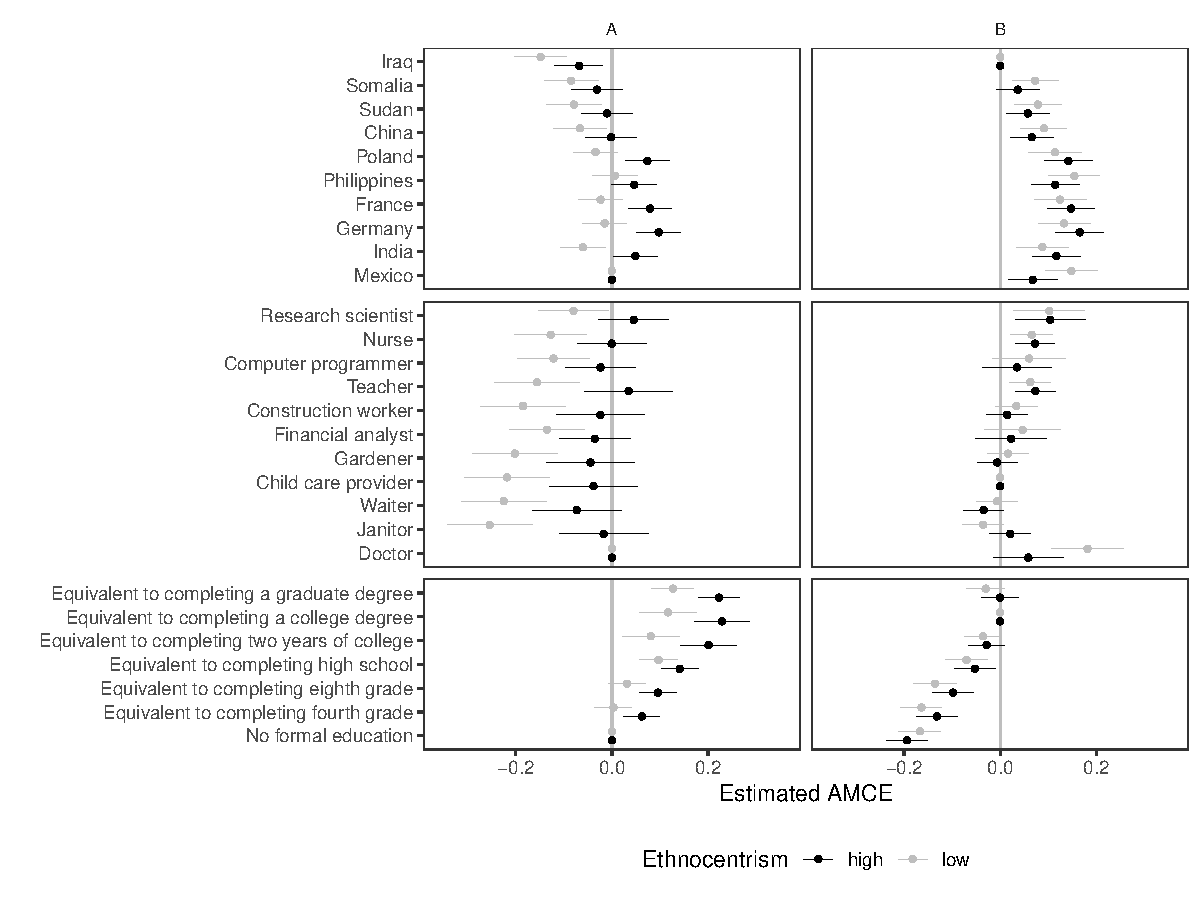
\includegraphics[width=\maxwidth]{figure/hainmueller_subgroup_example_plot-1} \caption[Comparison of AMCEs for Low- and High-Ethnocentrism Respondents Using Two Alternative Reference Categories Choices for Hainmueller et al]{Comparison of AMCEs for Low- and High-Ethnocentrism Respondents Using Two Alternative Reference Categories Choices for Hainmueller et al. (2014) Immigration Experiment}\label{fig:hainmueller_subgroup_example_plot}
\end{figure}


\end{knitrout}

We have shown that subgroup analyses of conjoint designs frequently entail the use of difference-in-AMCE comparisons and we have also shown that such analyses, counterintuitively, do not demonstrate differences in preferences between groups due the near-impossibility of selecting a non-arbitrary reference category against which to estimate AMCEs. Thus the choice of reference category --- while seemingly irrelevant --- has dramatic inferential consequences in conjoint analyses. Here we provide a more complete example, demonstrating the full extent of this problem for interpretation of conjoint results and present alternative forms of analysis that more robustly convey subgroup preferences and the differences (if any) between them. Consider the left and right facets of Figure \ref{fig:hainmueller_subgroup_example_plot}, which show the exact same analysis (comparing AMCEs for high and low ethnocentrism respondents) on the same experimental data from \citeauthor{HainmuellerHopkinsYamamoto2014}'s immigration experiment. In panel ``A'' (left), all features are configured so that the reference category is the one with the largest difference in preferences between the two subgroups. In panel ``B'' (right), all features are configured so that the reference category is the one with the smallest difference in preferences between the two subgroups.\footnote{The appendix contains comparable plots for experiments by \citet{BallardRosaMartinScheve2016} and \citet{TeeleKallaRosenbluth2018}.}

Panel A gives the impression that there are significant differences in preferences between high and low ethnocentrism respondents toward immigrants from different countries of origin, with different careers, and with different educational attainments. By contrast, Panel B gives the impression that these differences --- indeed all differences --- are negligible. The experimental data and analytic approach in the two portrayals is identical; the only difference is the choice of reference category for the profile features. Given what we have shown about the relationship between differences in conditional AMCEs and differences in conditional marginal means, Panel B is the more truthful visualization \citep{Cairo2016}. The differences between subgroup AMCEs there more accurately convey differences in underlying preferences because the reference categories used in Panel B are the most similar between the two groups. Yet even this may not \textit{perfectly} convey differences because no feature generates perfect agreement between the subgroups.

\begin{knitrout}
\definecolor{shadecolor}{rgb}{0.969, 0.969, 0.969}\color{fgcolor}\begin{figure}
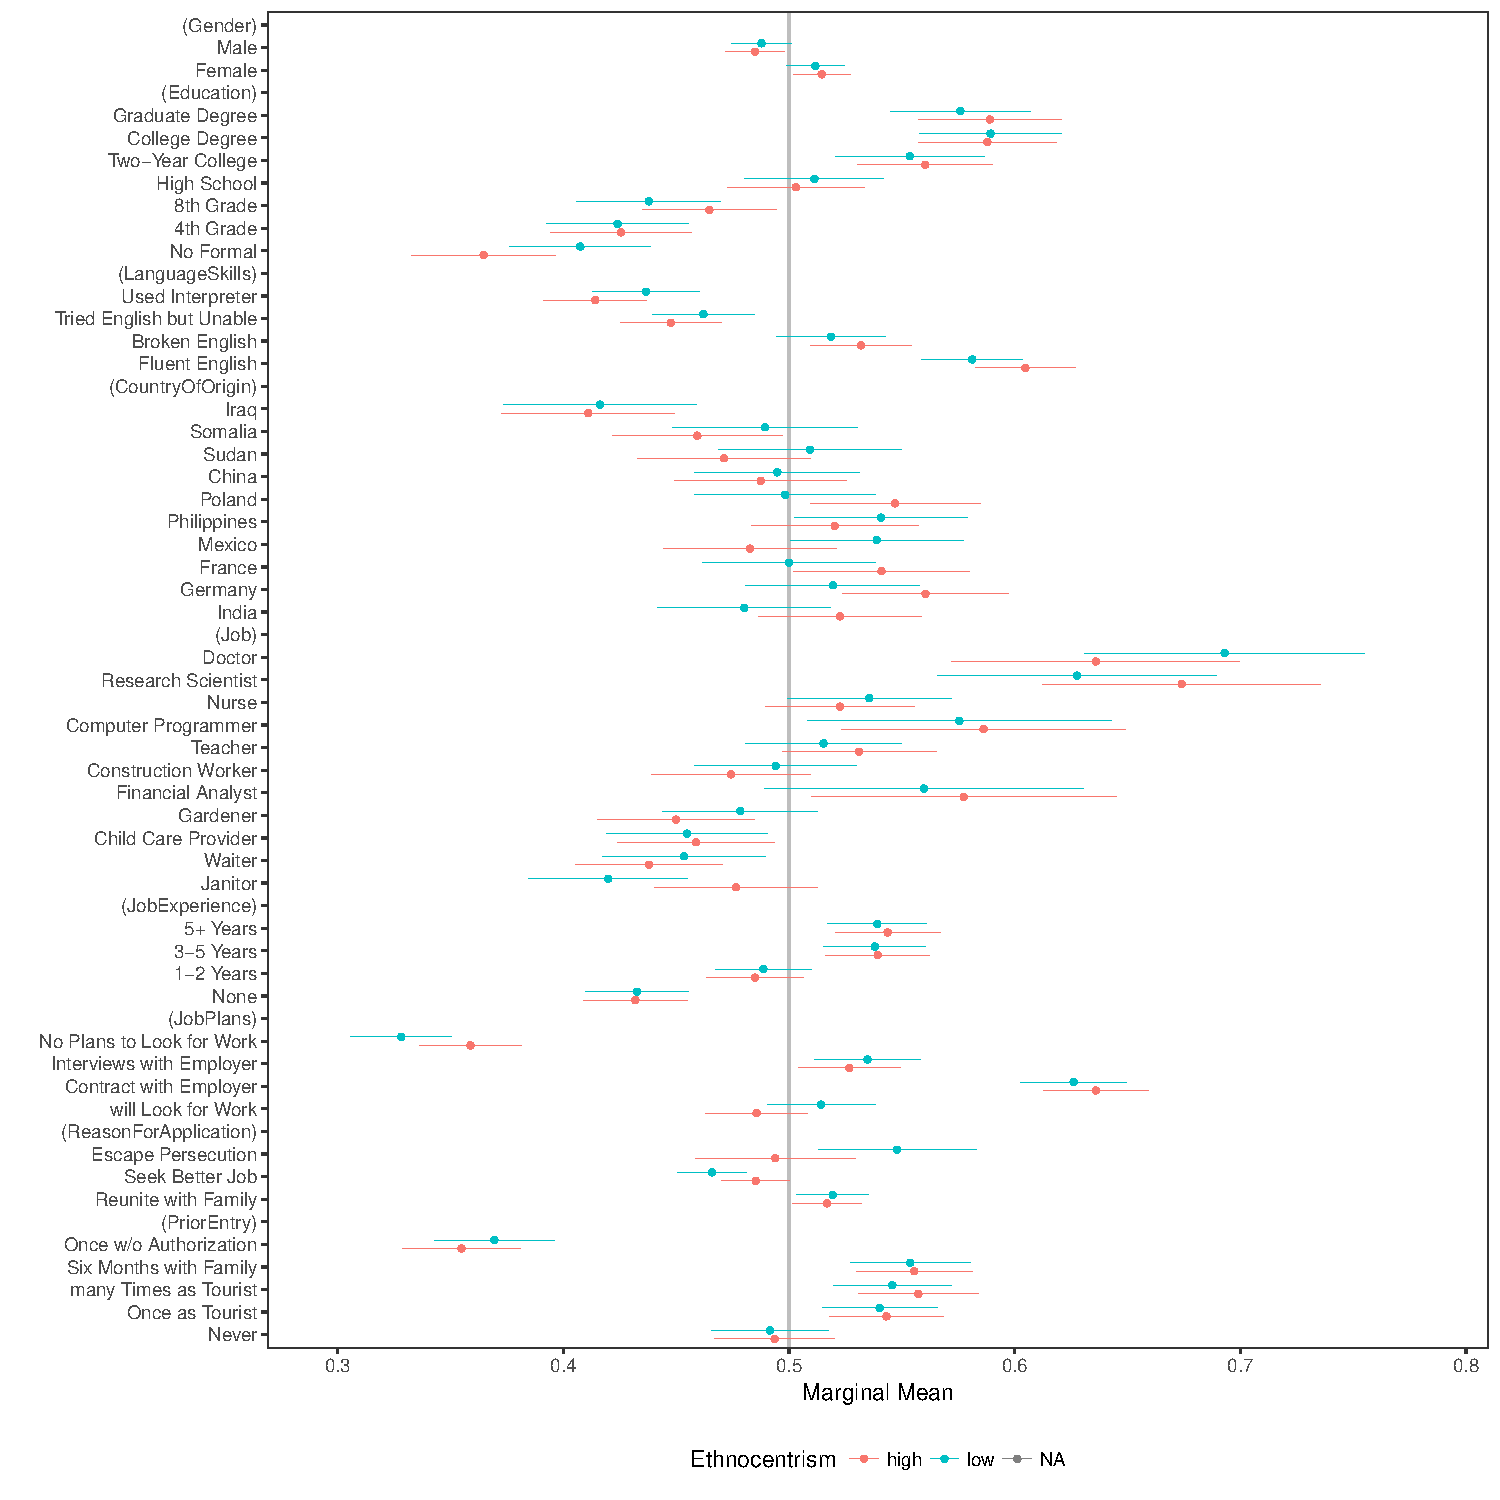
\includegraphics[width=\maxwidth]{figure/hainmueller_mm_by_ethnocentrism-1} \caption[Conditional Marginal Means, by Ethnocentrism, for Hainmueller et al.'s (2014) Immigration Experiment]{Conditional Marginal Means, by Ethnocentrism, for Hainmueller et al.'s (2014) Immigration Experiment}\label{fig:hainmueller_mm_by_ethnocentrism}
\end{figure}


\end{knitrout}

\begin{knitrout}
\definecolor{shadecolor}{rgb}{0.969, 0.969, 0.969}\color{fgcolor}\begin{figure}
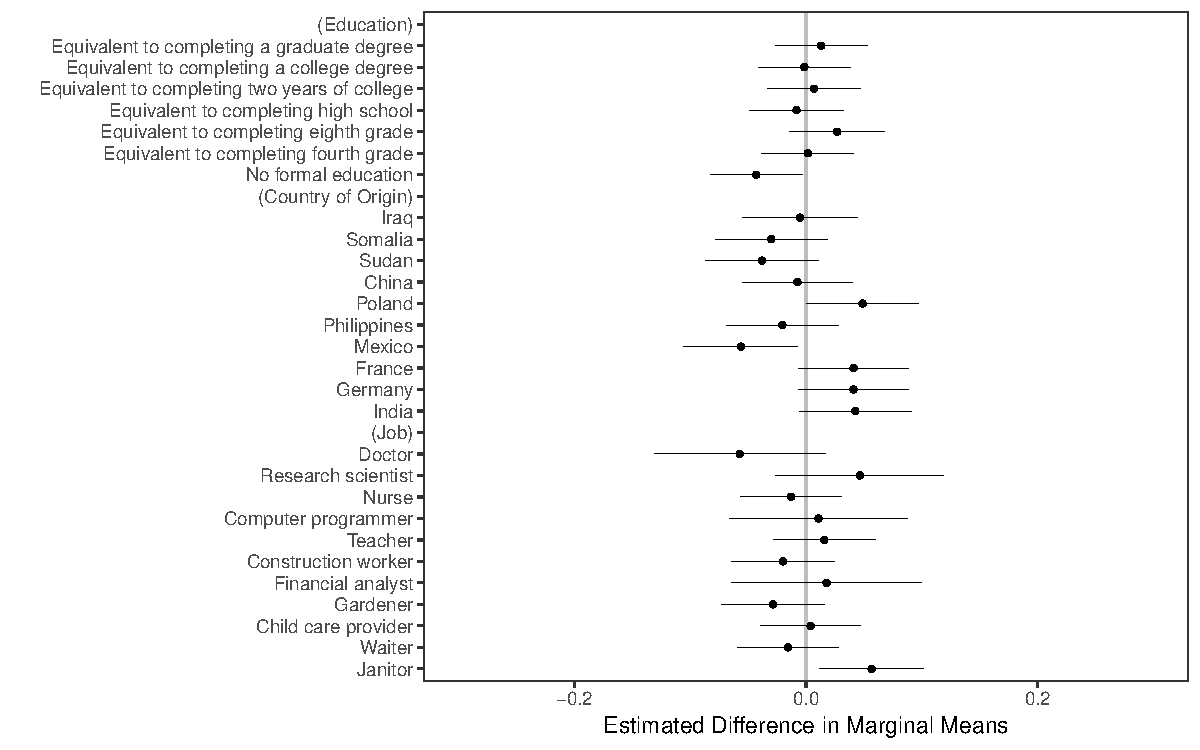
\includegraphics[width=\maxwidth]{figure/hainmueller_mm_diffs-1} \caption[Differences in Conditional Marginal Means, by Ethnocentrism, for Hainmueller et al.'s (2014) Immigration Experiment]{Differences in Conditional Marginal Means, by Ethnocentrism, for Hainmueller et al.'s (2014) Immigration Experiment}\label{fig:hainmueller_mm_diffs}
\end{figure}


\end{knitrout}

Alternatively presenting subgroup differences using conditional marginal means (as in Figure \ref{fig:hainmueller_mm_by_ethnocentrism}) provides the intended descriptive comparison of subgroup preferences. Each dot and error bar represents the conditional marginal mean (and its standard error) for high ethnocentrism (in red) and low ethnocentrism (in blue) respondents. This display of conditional marginal means highlights just how similar the preferences are for the two groups. For example, in the first set of estimates, both groups of respondents display minimally positive preferences toward female immigrants and minimally negative preferences toward male immigrants, averaging across those immigrants' other profile features. The second set of estimates shows both group are also more favorable toward higher-educated immigrants and less favorable toward less-education immigrants with no visually apparent differences. The third set of estimates, related to language skills, shows again similar patterns: both groups are more favorable toward immigrants with higher English proficiency than immigrants with lower English proficiency.

These estimates are less obviously identical for the two groups but look quite close. To test for pairwise differences between high and low ethnocentrism respondents, we can calculate differences in conditional conditional marginal means at each feature level, with associated significance tests:

\begin{itemize}
\item spoke fluent English: 0.02 (0.02, $z_{\text{diff}}$=1.30, $p\leq 0.20$)
\item spoke broken English: 0.01 (0.02, $z_{\text{diff}}$=0.71, $p\leq 0.48$)
\item tried to speak English but was unable: -0.01 (0.02, $z_{\text{diff}}$=-0.78, $p\leq 0.43$)
\item spoke [language] and used an interpreter: -0.02 (0.02, $z_{\text{diff}}$=-1.22, $p\leq 0.22$)

\end{itemize}



\noindent These pairwise tests show that are our eyes have not deceived us. None of the level-specific differences in conditional marginal means are statistically distinguishable from zero. Were we interested in an omnibus tests of whether any of these differences were non-zero, we could perform a nested model comparison of two equations: (a) one estimating only marginal effects of the ``Language Skills'' feature, and (b) the same model with additional interactions between the subgrouping covariate and the features. The resulting F-test for the model comparison in this case again gives us little reason to believe there are subgroup differences: F(4)=1.06, $p\leq0.37$. We could repeat such pairwise comparisons or omnibus comparisons for each feature in the design.

Furthermore, we could also directly visualize differences in conditional marginal means for this feature --- and all features --- as in Figure \ref{fig:hainmueller_mm_diffs}. This provides a more direct presentation of \textit{differences} between subgroup preferences as the vertical line indicates feature levels for which there is no difference between the two groups. Positive values to the right of the line indicate positive differences (high ethnocentrism respondents are more favorable toward immigrants with this feature than low ethnocentrism respondents) and negative value to the left of zero convey the opposite. A further advantage of this plot is that unlike displays of conditional AMCEs, differences in conditional marginal means communicate subgroup differences for all feature levels including the reference categories. This display makes readily clear what was only indirectly apparent in Figure \ref{fig:hainmueller_mm_by_ethnocentrism}: there are indeed no sizeable and only a few statistically apparent differences in preferences between the two groups.



As before, we can perform an omnibus tests for the presence of any subgroup differences across all features, again using nested model comparison of two equations: (a) one estimating only effects of the features, and (b) the same model with additional interactions between the subgrouping covariate and all features. The result of that test for differences by ethnocentrism from the immigration experiment is: F(98)=1.16, $p\leq0.14$, which further demonstrates that the substantive interpretation provided by \citet{HainmuellerHopkinsYamamoto2014} accurately identified a lack of between-group differences. This kind of test can also be used to assess heterogeneity across conjoint features. For example, \citet{TeeleKallaRosenbluth2018} report just such a test for how effects of features other than candidate sex may differ between male and female candidates, finding no such heterogeneity (8--9). Fortunately, the original analysis accurately detected an absence of subgroup differences, yet a subtly different set of analytic decisions about reference categories (as shown in Figure \ref{fig:hainmueller_subgroup_example_plot}) could have led to an quite different conclusion.

\section*{Conclusion}\label{sec:conclusion}

This article has identified several challenges related to the analysis and reporting of conjoint experimental designs, particularly analyses of subgroup differences. We suggest that conjoint analyses should report not only average marginal component effects (AMCEs) but also descriptive quantities that better convey underlying preferences over profile features and better convey subgroup differences in those preferences. Our intention here is not to substantively undermine any previous set of results but instead to urge researchers moving forward to demonstrate considerable caution in how they design, analyze, and present the results of these types of experiments. We have relatively straightforward and hopefully uncontroversial advice for how analysts of conjoint experiments should proceed:

\begin{enumerate}
\item Always report unadjusted marginal means when attempting to provide a \textit{descriptive} summary of respondent preferences in addition to or instead of AMCEs.\footnote{Like the presentation of AMCEs, displaying marginal means in constrained conjoint designs may also distort apparent patterns given that not all features can co-occur. Partitioning the design into fractions such that each fraction contains a fully unconstrained design would mitigate any concern with that presentation.}

\item Exercise caution when explicitly or implicitly interpreting differences-in-AMCEs across subgroups. While that quantity conveys the difference in effects of a change in a given feature, heterogeneous effects do not necessarily mean different underlying preferences. Differences-in-AMCEs are almost always a biased estimate (of unknown sign and direction) of the difference in underlying preferences. If differences in AMCEs are reported, the choice of reference categories should be discussed explicitly and diagnostics should be provided to justify it.

\item When descriptively characterizing differences in preferences between subgroups, directly estimate the subgroup difference using conditional marginal means and differences between conditional marginal means, rather than relying on the difference-in-AMCEs.

\item To formally test for group differences in preferences, regression with interaction terms between the subgrouping covariate and all feature levels will generate estimates of level-specific differences in preferences via the coefficients on the interaction terms.\footnote{The analysis is slightly more complicated in constrained designs.} A nested model comparison between this equation against one without such interactions provides an omnibus test of subgroup differences, which should be reported when characterizing overall patterns of subgroup differences.
\end{enumerate}

\noindent Following this advice, we hope, will allow researchers to more clearly and more accurately represent descriptive results of conjoint experiments.

The popularity of conjoint analyses in recent years highlights the power of the design and the important contributions made by \citet{HainmuellerHopkinsYamamoto2014} in providing a novel causal interpretation of these fully randomized factorial designs. Yet with new tools always come new challenges. The now-common practice of descriptively interpreting conjoints requires more caution than is immediately obvious. This paper has demonstrated several such challenges and hopefully provides useful advice for how researchers should proceed with the analysis of such designs.

To facilitate such analysis and, especially, to provide easy-to-use tools for calculating marginal means and performing reference category selection diagnostics, we provide software called \textbf{cregg} \citep{Leeper2018cregg} that will perform these analyses and also provides the simple-to-use visualization tools used throughout this article. With that resource in-hand, researchers should be well-equipped to analyze conjoint designs without running into the analytic challenges discussed here.



\singlespacing
\bibliographystyle{apsa-leeper}
\bibliography{references}
\clearpage


\appendix
\tableofcontents



\clearpage

\section{Definition of Quantities of Interest}\label{app:quantities}

A conjoint experiment serves two purposes: (1) description of the conditional distribution of favorability over variations in multiple features, and (2) leveraging the random observation of combinations of features (so-called ``profiles'') to infer that any differences in favorability over features are causally attributable to the features as opposed to something else. The quantities of interest are therefore functions of the features being randomized as in any factorial experiment. But additionally, conjoints typically involve within-subjects research designs (i.e., multiple, different profile observations per participant) thus necessitating some additional notation to account for the \textit{survey implementation} of the conjoint in addition to the definition of the descriptive and causal parameters of interest.

Ultimately, a conjoint since \citet{HainmuellerHopkinsYamamoto2014} is a complex survey-experimental design involving multiple observations across a high-dimension factorial experimental space. Specifically, $I$ respondents ($i \in \{1, \dots, I\}$) are presented with $K$ rating or forced choice decision tasks, each involving $J$ (typically 2) alternative profiles of, for example, candidates or policies. Each profile consists of a vector of $F$ (typically discrete) features or attributes that describe the profile (e.g., age, sex), each composed of $D_f$ alternative levels, a number which can vary across features. The experiment thus generates a dataset with $N = I \times J \times K$ observations of some rating scale or discrete choice outcome, $Y$, from a random sample of profiles drawn from the $C = \prod_{f = 1}^{F} D_f$ population of experimental \textit{cells} in the $F$-dimension feature space.

The survey implementation of the conjoint therefore generates $N$ observations that can be indexed by $i,j,k$, forming an $N \times(L+4)$ dimensional data matrix $\mathbf{M}$ with each row representing the vector of feature levels $\vec{F}$ in each profile $j$ of respondent $i$'s task $k$, with indicators for $i$, $j$, $k$, and the corresponding outcome $Y_{i,j,k}$.\footnote{In typical paired designs (where $J=2$), this means each task generates two data points: $Y_{i,1,k}$ and $Y_{i,2,k}$. Note, too, that in fully randomized designs, these two profiles can be identical. Furthermore in fully randomized, forced-choice designs this can yield the additional curiosity that $Y_{i,\mathbf{c}} \neq Y_{i,\mathbf{c}}$ for a given respondent, $i$, and profile, $\mathbf{c}$.}

With no loss of information, we can think of each row in this matrix equivalently as an observation of $Y_{i,\vec{F}}$. This is because \citet{HainmuellerHopkinsYamamoto2014} make several important assumptions that allow us to interpret these data in a different way than the survey implementation implies. First, they assume no carryover effects (Assumption 1), such that multiple observations from the same respondent can be treated as independent of one another. Second, they assume no profile order effects within-task (Assumption 2), such that profiles within a task can be treated as independent of each other. Assumptions 1 and 2 imply that the survey implementation indices for task, $k$, and profile-within-task, $j$, can be ignored. They have no bearing on any quantity of interest, by assumption. 

The analyst is therefore left with a dataset of $N$ observations, grouped into $i$ participants, each providing into $Y_{\vec{F}}$. All quantities of interest must therefore be specified over as features of the distribution of $Y$ over the $F$-dimensional feature space. In what follows, we therefore focus on the experimental features being randomized rather than the survey design factors being assumed away. \citet{HainmuellerHopkinsYamamoto2014} make a third assumption that profiles are randomly constituted (Assumption 3), which in a fully randomized design, has the effect of meaning that features and feature combinations are randomly sampled for observation. If this randomization is uniform (which it almost always is in applied examples) this means we can additionally ignore the probability of observing any given combination (as all profiles are equally likely to be observed). This is a point we return to in a moment.

The most basic thing that can be learned about the distribution of $Y$ is the expected value, $E[Y]$, or \textit{grand mean} (in the parlance of factorial experiments). We can think of this quantity in terms of the survey implementation process (namely, respondents, tasks, and profiles) or as a simple function of the resulting data:

\begin{equation}
\bar{Y} = \dfrac{1}{I \times J \times K} \sum_{i=1}^{I} \sum_{j=1}^{J} \sum_{k=1}^{K} Y_{i,j,k} = \dfrac{1}{N} \sum_{n=1}^{N} Y_n
\end{equation}

\noindent The nested summation over $i,j,k$ could be stated explicitly but is unnecessary as the grand mean is simply the mean of all observed $Y$. A useful check on intuition is that in a forced choice design, where a respondent must choose only one profile, $j$, of all those presented in each task $k$, then by design $\bar{Y} = \frac{1}{J}$. For common, two-alternative, forced choice designs, $\bar{Y}$ therefore always equals $0.5$. By contrast, in rating scale designs, $\bar{Y}$ can take any value between the lower and upper bounds of the rating scale.

In an experiment where $N > C$ (the number of observations is large than the number of cells) due to a large sample, or few factors, or levels of each factor, or both (or both of these design characteristic), a sensible next quantity of interest is the \textit{cell mean}: $E[Y|\vec{X} = \vec{x}]$, which in a conjoint simply measures the mean favorability toward a particular profile, $\vec{x}$. An effort to actually estimate this quantity will, however, become obviously intractable when one recognizes that the number of observations in a typical conjoint is much lower the number of feasible profiles ($N \ll C$). The cell mean can be unobserved for many or perhaps most experimental cells. 

Therefore quantities of interest that derive from it --- such as pairwise differences of means between cells --- cannot be estimated for any of the arbitrary $\binom{C}{2}$ pairs of cells. As an example, in the \cite{HainmuellerHopkinsYamamoto2014} candidate experiment, $C = 6^6 * 2^2 = 186,624$ and $N = 3466$, so less than 2\% of experimental cells were observable and a minuscule fraction of the 17.4 billion pairwise cell combinations could have generated estimable effects. 

It is at this point that the quantities of interest in a conjoint can become confusing. In a typical experiment where $N > C$, these pairwise differences of means are the standard estimator for a causal effect. For example, we might be interested in the effect on $Y$ of changing the value of one feature to another theoretically interesting value of that feature, holding all other feature values in the profile constant:

\begin{equation}
\tau = E[Y|X_1=x_1,X_2=x_2,\dots,X_f=x_f] - E[Y|X_1= \neg x_1,X_2=x_2,\dots,X_f=x_f]
\end{equation}

\noindent but we have no guarantee that both or, in fact, either of those particular cells are observed. If even this minimal causal quantity cannot be guaranteed to be estimable by design, questions about higher-order interactions across features are even more difficult to estimate as they require observing four or more specific cells, any of which may be missing. Even if we were interested in such quantities, we would be unlikely to be able to estimate them.

Conjoint designs therefore ask us to think about completely different quantities of interest from typical sentiment measurement or experimentation. Consequently, what quantities might we care about that can be estimated from an $L$-dimension factorial experimental with considerable sparsity other than the grand mean? 

Even though $N \ll C$ in most applied conjoints, $N > F$. This means that even if we probably cannot learn about particular high-dimensional \textit{combinations of features}, we can learn about favorability toward particular features alone. That is, we can learn about conditional expectations over each feature dimension, $E[Y|X_f=x_f]$. In the factorial experiments literature, this conditional mean is called the \textit{marginal mean} (as it lies at the margins of a tabular presentation cell means for the complete design). The uniform sampling of cells in the design means that this is quantity can be estimated by the simple mean of $Y \forall X_f = x_f$. Were a constrained conjoint design used where some feature combinations were impossible, the marginal means would only be intelligible in the fractions of the design where all cells are observed.\footnote{Practically, the random sampling of cells does not need to be uniform; over- and under-representation of cells is possible. We focus here on fully randomized designs that draw profiles from the full space with equal probability. A nuance in \citeauthor{HainmuellerHopkinsYamamoto2014}'s notation is that their quantities of interest are conditioned on an arbitrary joint distribution of features rather than the particular joint distribution of features that was used to construct design or the joint distribution of features that happens to emerge empirically. In other words, they weight cells by an arbitrary joint probability mass function.}

To clarify this point, consider the constrained 2x3 design below where one cell is unobserved by design:

\begin{center}
\begin{tabular}{lccc}\toprule
 & $A = 1$ & $A = 2$ & \\ \midrule
$B = 1$ & $Y_{A=1, B=1}$ & $Y_{A=2, B=1}$ & $E[Y|B=1]$ \\
$B = 2$ & $Y_{A=1, B=2}$ & $Y_{A=2, B=1}$ & $E[Y|B=2]$ \\
$B = 3$ & $Y_{A=1, B=3}$ & -- & $E[Y|B=3]$ \\ \midrule
 & $E[Y|A=1]$ & $E[Y|A=2]$ & $E[Y]$ \\ \bottomrule
\end{tabular}
\end{center}

\noindent Were the lower-right cell ($A=2, B=3$) observable by design, then a direct comparison of the marginal means, $E[Y|A=1]$ and $E[Y|A=2]$, in the lower table margin would provide direct insight into the relative favorability of respondents to profiles with features $A=1$ and $A=2$, marginalized over $B$. But because this cell is unobserved, these marginal means marginalize over different subsets of the possible values of $B$ making them not obviously comparable. By contrast, the first and second marginal means at the top-right of the table --- $E[Y|B=1]$ and $E[Y|B=2]$ --- provide insight into the favorability of participants toward profiles with features $B=1$ and with feature $B=2$ marginalizing over the two possible values of $A$. A researcher could safely conclude that participants are more (less) favorable toward profiles with feature $B=1$ than $B=2$ from this information alone. But they would not be able to so for feature $A$ without either (a) an explicit caveat that the comparison is of dissimilar subsets of profiles along dimension $B$ or (b) calculating marginal means over only the completely observable\footnote{Note that what matters here is \textit{observability}, not whether any given cell is actually observed. We know from above that most cells will be unobserved even in a uniformly sampled, unconstrained design.} portion of the feature space.

For the common \textit{descriptive} use of conjoint designs to measure preferences over multi-dimensional objects, these marginal means alone are of direct interest. They express favorability on the scale of the outcome over alternative values of each feature.

For the \textit{causal} interpretation of conjoint designs, comparisons of these marginal means is required. Comparisons between them provide causal inferences about the effect of changing a focal feature, marginalizing across the distribution of other features. Because feature combinations (i.e., the profiles) are randomly constructed and randomly observed from all possible combinations, the distribution of other non-focal features is, in expectation, is independent of the focal feature, thus identical across all levels of the focal feature, and therefore ignorable. A typical causal effect of interest is therefore the difference in marginal means across two levels of a feature. For an unconstrained design, this difference is the \textit{average marginal component effect} (AMCE) defined by \citet{HainmuellerHopkinsYamamoto2014}. In this way, an AMCE is simply a marginal effect of the factorial design: the difference of two marginal means.

Unfortunately, this is not a perfectly complete definition, but it covers the vast majority of applied cases. The exceptions are few. First, \citeauthor{HainmuellerHopkinsYamamoto2014} allow the joint distribution of features used in calculating the difference of marginal means to be arbitrary. This is meant to accommodate the weighting of effects to reflect the real-world distribution of feature combinations (e.g., down-weighting African American Republican political candidates given their rarity in real-world politics) but in practice this is uncommon.

Second, in constrained designs where some cells are unobservable, care needs to be taken in both defining and estimating AMCEs. Take, for example, the trivial example just above. The difference $E[Y|B=2]-E[Y|B=1]$ marginalizes over the full set of levels of $A$ but $E[Y|B=3]-E[Y|B=1]$ marginalizes only over case where $A=1$. \citeauthor{HainmuellerHopkinsYamamoto2014} allow for these two differences to be presented as the AMCE despite the fact that the quantities marginalize over distinct subsets of the design. For example, if feature $A$ is race ${Caucasian, African American}$ and feature $B$ is religion ${Evangelical, Catholic, Jewish}$. In \citeauthor{HainmuellerHopkinsYamamoto2014}'s notation, the AMCE of a candidate being Jewish relative to being Evangelical Christian is defined only for Caucasian candidates, while the AMCE of being Catholic is defined for both African American and Caucasian candidates. There is nothing inherently problematic about that but, as noted earlier, it requires either being clear about what features are being marginalized over or an analysis of only the complete and comparable subset of the design. So, researchers using such designs may prefer to not present the AMCE of being Jewish together with the other results as it does not draw upon the complete set of feature combinations used in other portions of the analysis.



\clearpage

\section{Hainmueller et al. (2014) Immigration Experiment}

\subsection{Replication using AMCEs}

\begin{knitrout}
\definecolor{shadecolor}{rgb}{0.969, 0.969, 0.969}\color{fgcolor}
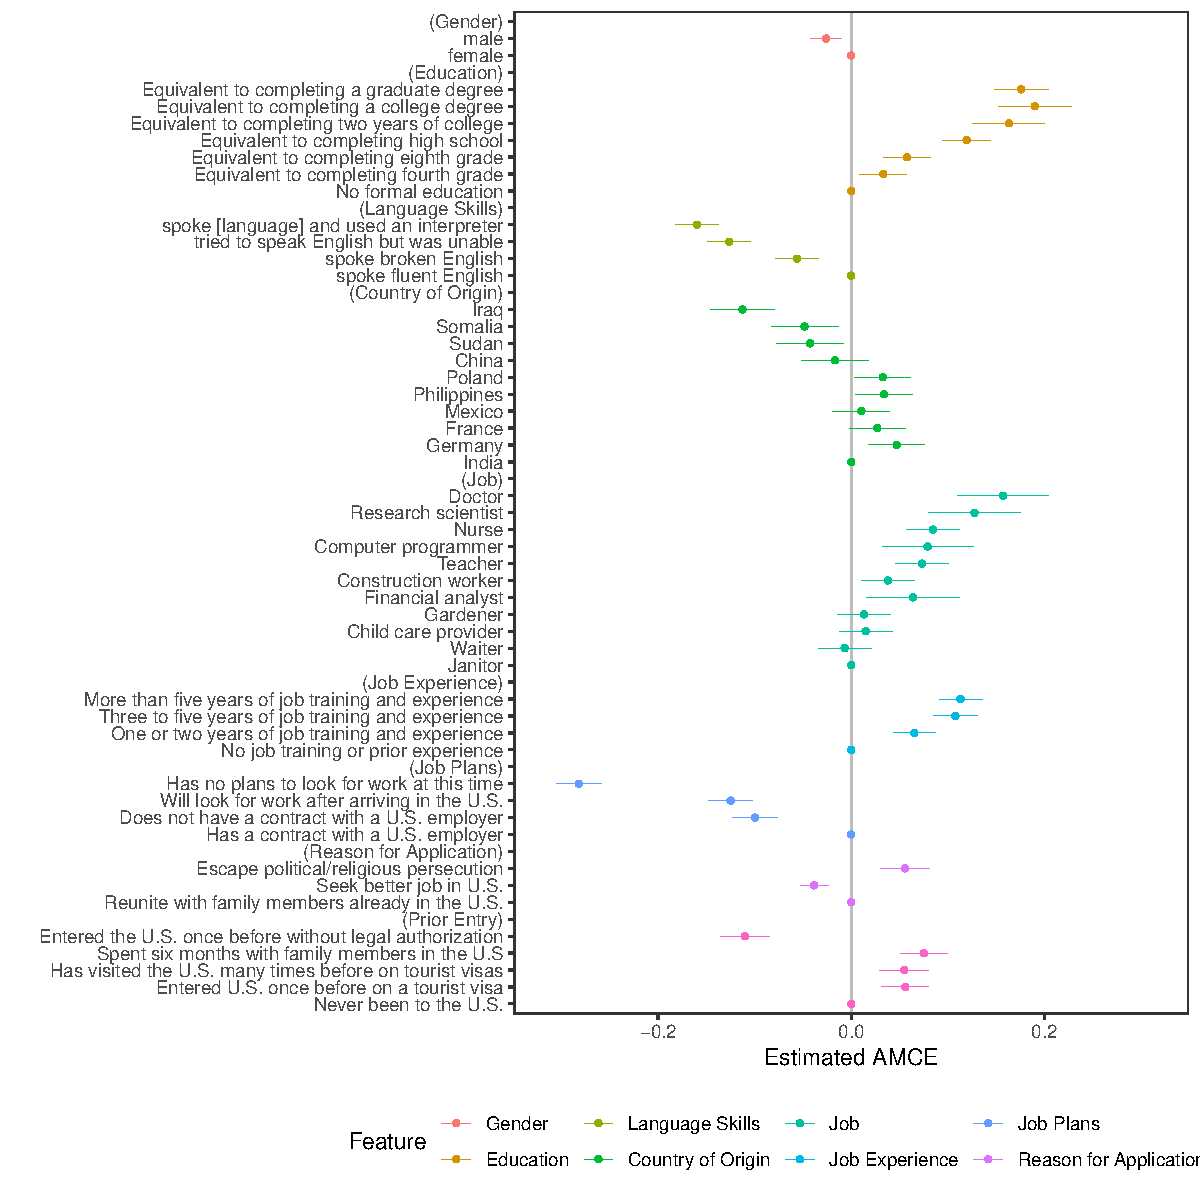
\includegraphics[width=\maxwidth]{figure/hainmueller_immigration_amce_appendix-1} 

\end{knitrout}

\clearpage

% latex table generated in R 3.5.1 by xtable 1.8-3 package
% Sun Nov 25 10:42:30 2018
\begin{table}[ht]
\centering
\begingroup\footnotesize
\begin{tabular}{lp{3in}rrr}
  \hline
feature & level & estimate & std.error & z \\ 
  \hline
Gender & female & 0.00 &  &  \\ 
  Gender & male & -0.03 & 0.01 & -3.25 \\ 
  Education & No formal education & 0.00 &  &  \\ 
  Education & Equivalent to completing fourth grade & 0.03 & 0.01 & 2.22 \\ 
  Education & Equivalent to completing eighth grade & 0.06 & 0.01 & 3.86 \\ 
  Education & Equivalent to completing high school & 0.12 & 0.01 & 7.98 \\ 
  Education & Equivalent to completing two years of college & 0.16 & 0.02 & 7.12 \\ 
  Education & Equivalent to completing a college degree & 0.19 & 0.02 & 8.26 \\ 
  Education & Equivalent to completing a graduate degree & 0.18 & 0.02 & 10.41 \\ 
  Language Skills & spoke fluent English & 0.00 &  &  \\ 
  Language Skills & spoke broken English & -0.06 & 0.01 & -4.98 \\ 
  Language Skills & tried to speak English but was unable & -0.13 & 0.01 & -11.11 \\ 
  Language Skills & spoke [language] and used an interpreter & -0.16 & 0.01 & -13.78 \\ 
  Country of Origin & India & 0.00 &  &  \\ 
  Country of Origin & Germany & 0.05 & 0.02 & 2.66 \\ 
  Country of Origin & France & 0.03 & 0.02 & 1.53 \\ 
  Country of Origin & Mexico & 0.01 & 0.02 & 0.59 \\ 
  Country of Origin & Philippines & 0.03 & 0.02 & 1.91 \\ 
  Country of Origin & Poland & 0.03 & 0.02 & 1.83 \\ 
  Country of Origin & China & -0.02 & 0.02 & -0.81 \\ 
  Country of Origin & Sudan & -0.04 & 0.02 & -2.01 \\ 
  Country of Origin & Somalia & -0.05 & 0.02 & -2.29 \\ 
  Country of Origin & Iraq & -0.11 & 0.02 & -5.56 \\ 
  Job & Janitor & 0.00 &  &  \\ 
  Job & Waiter & -0.01 & 0.02 & -0.41 \\ 
  Job & Child care provider & 0.01 & 0.02 & 0.89 \\ 
  Job & Gardener & 0.01 & 0.02 & 0.78 \\ 
  Job & Financial analyst & 0.06 & 0.03 & 2.17 \\ 
  Job & Construction worker & 0.04 & 0.02 & 2.26 \\ 
  Job & Teacher & 0.07 & 0.02 & 4.39 \\ 
  Job & Computer programmer & 0.08 & 0.03 & 2.76 \\ 
  Job & Nurse & 0.08 & 0.02 & 5.08 \\ 
  Job & Research scientist & 0.13 & 0.03 & 4.44 \\ 
  Job & Doctor & 0.16 & 0.03 & 5.49 \\ 
  Job Experience & No job training or prior experience & 0.00 &  &  \\ 
  Job Experience & One or two years of job training and experience & 0.07 & 0.01 & 5.92 \\ 
  Job Experience & Three to five years of job training and experience & 0.11 & 0.01 & 9.32 \\ 
  Job Experience & More than five years of job training and experience & 0.11 & 0.01 & 9.96 \\ 
  Job Plans & Has a contract with a U.S. employer & 0.00 &  &  \\ 
  Job Plans & Does not have a contract with a U.S. employer & -0.10 & 0.01 & -8.50 \\ 
  Job Plans & Will look for work after arriving in the U.S. & -0.12 & 0.01 & -10.69 \\ 
  Job Plans & Has no plans to look for work at this time & -0.28 & 0.01 & -23.91 \\ 
  Reason for Application & Reunite with family members already in the U.S. & 0.00 &  &  \\ 
  Reason for Application & Seek better job in U.S. & -0.04 & 0.01 & -4.37 \\ 
  Reason for Application & Escape political/religious persecution & 0.06 & 0.02 & 3.58 \\ 
  Prior Entry & Never been to the U.S. & 0.00 &  &  \\ 
  Prior Entry & Entered U.S. once before on a tourist visa & 0.06 & 0.01 & 4.49 \\ 
  Prior Entry & Has visited the U.S. many times before on tourist visas & 0.05 & 0.01 & 4.24 \\ 
  Prior Entry & Spent six months with family members in the U.S & 0.08 & 0.01 & 5.98 \\ 
  Prior Entry & Entered the U.S. once before without legal authorization & -0.11 & 0.01 & -8.45 \\ 
   \hline
\end{tabular}
\endgroup
\end{table}


\clearpage

\subsection{Replication using MMs}

\begin{knitrout}
\definecolor{shadecolor}{rgb}{0.969, 0.969, 0.969}\color{fgcolor}
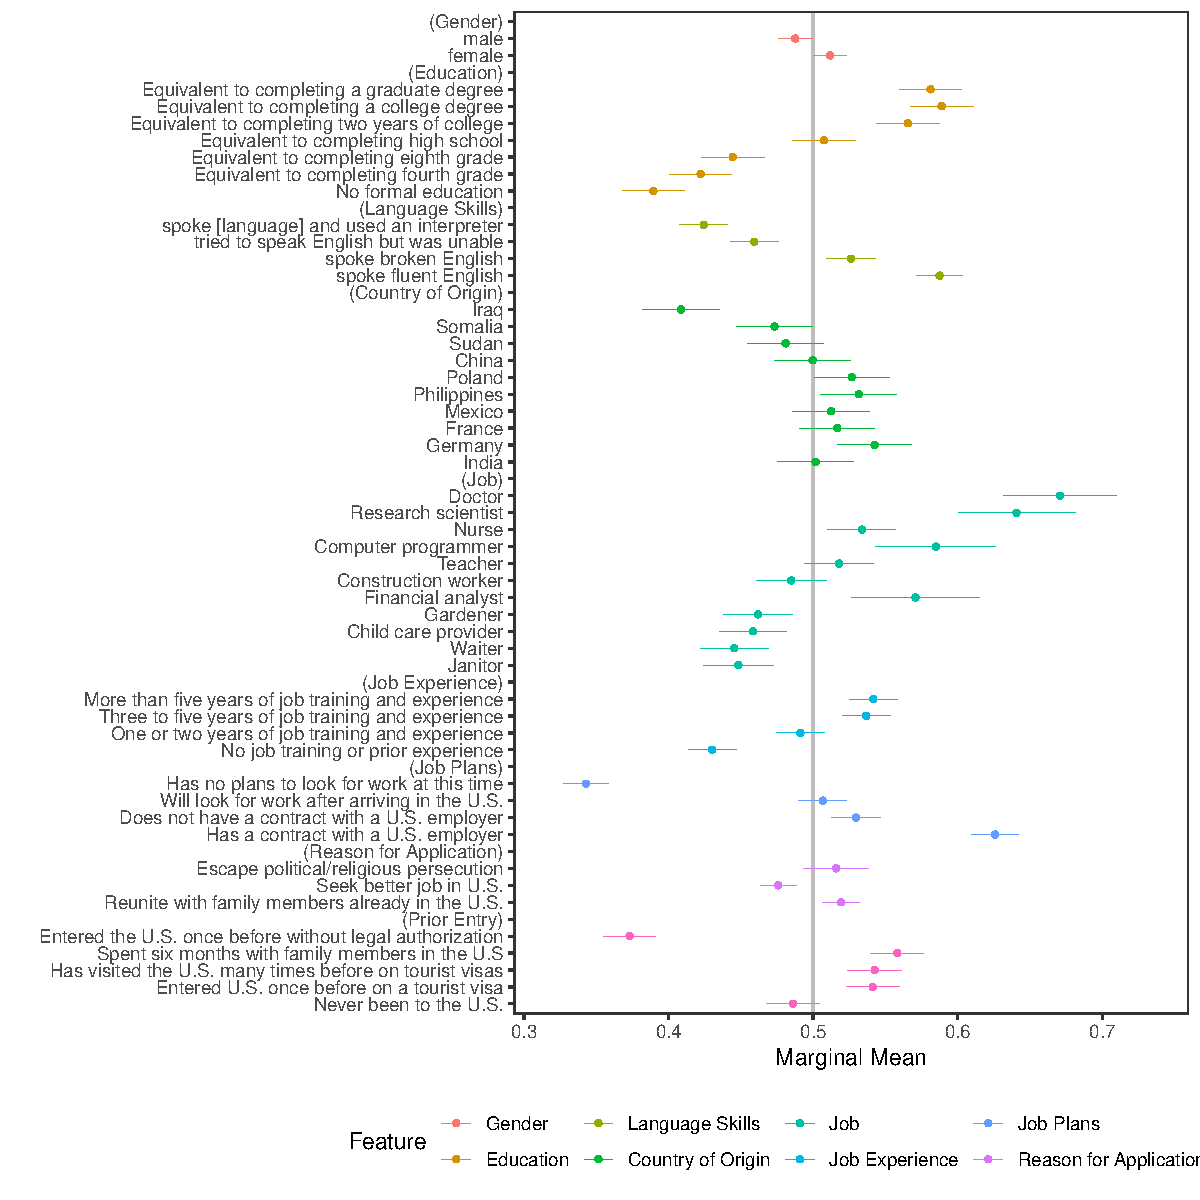
\includegraphics[width=\maxwidth]{figure/hainmueller_immigration_mm_appendix-1} 

\end{knitrout}

\clearpage

% latex table generated in R 3.5.1 by xtable 1.8-3 package
% Sun Nov 25 10:42:36 2018
\begin{table}[ht]
\centering
\begingroup\footnotesize
\begin{tabular}{lp{3in}rrr}
  \hline
feature & level & estimate & std.error & z \\ 
  \hline
Gender & female & 0.51 & 0.01 & 1.99 \\ 
  Gender & male & 0.49 & 0.01 & -2.03 \\ 
  Education & No formal education & 0.39 & 0.01 & -10.04 \\ 
  Education & Equivalent to completing fourth grade & 0.42 & 0.01 & -7.08 \\ 
  Education & Equivalent to completing eighth grade & 0.44 & 0.01 & -5.00 \\ 
  Education & Equivalent to completing high school & 0.51 & 0.01 & 0.67 \\ 
  Education & Equivalent to completing two years of college & 0.57 & 0.01 & 5.92 \\ 
  Education & Equivalent to completing a college degree & 0.59 & 0.01 & 8.00 \\ 
  Education & Equivalent to completing a graduate degree & 0.58 & 0.01 & 7.40 \\ 
  Language Skills & spoke fluent English & 0.59 & 0.01 & 10.63 \\ 
  Language Skills & spoke broken English & 0.53 & 0.01 & 3.07 \\ 
  Language Skills & tried to speak English but was unable & 0.46 & 0.01 & -4.83 \\ 
  Language Skills & spoke [language] and used an interpreter & 0.42 & 0.01 & -8.98 \\ 
  Country of Origin & India & 0.50 & 0.01 & 0.13 \\ 
  Country of Origin & Germany & 0.54 & 0.01 & 3.22 \\ 
  Country of Origin & France & 0.52 & 0.01 & 1.26 \\ 
  Country of Origin & Mexico & 0.51 & 0.01 & 0.92 \\ 
  Country of Origin & Philippines & 0.53 & 0.01 & 2.36 \\ 
  Country of Origin & Poland & 0.53 & 0.01 & 2.01 \\ 
  Country of Origin & China & 0.50 & 0.01 & -0.03 \\ 
  Country of Origin & Sudan & 0.48 & 0.01 & -1.42 \\ 
  Country of Origin & Somalia & 0.47 & 0.01 & -2.01 \\ 
  Country of Origin & Iraq & 0.41 & 0.01 & -6.76 \\ 
  Job & Janitor & 0.45 & 0.01 & -4.20 \\ 
  Job & Waiter & 0.45 & 0.01 & -4.56 \\ 
  Job & Child care provider & 0.46 & 0.01 & -3.50 \\ 
  Job & Gardener & 0.46 & 0.01 & -3.11 \\ 
  Job & Financial analyst & 0.57 & 0.02 & 3.16 \\ 
  Job & Construction worker & 0.48 & 0.01 & -1.23 \\ 
  Job & Teacher & 0.52 & 0.01 & 1.49 \\ 
  Job & Computer programmer & 0.58 & 0.02 & 4.01 \\ 
  Job & Nurse & 0.53 & 0.01 & 2.82 \\ 
  Job & Research scientist & 0.64 & 0.02 & 6.82 \\ 
  Job & Doctor & 0.67 & 0.02 & 8.53 \\ 
  Job Experience & No job training or prior experience & 0.43 & 0.01 & -8.27 \\ 
  Job Experience & One or two years of job training and experience & 0.49 & 0.01 & -1.05 \\ 
  Job Experience & Three to five years of job training and experience & 0.54 & 0.01 & 4.33 \\ 
  Job Experience & More than five years of job training and experience & 0.54 & 0.01 & 4.92 \\ 
  Job Plans & Has a contract with a U.S. employer & 0.63 & 0.01 & 15.40 \\ 
  Job Plans & Does not have a contract with a U.S. employer & 0.53 & 0.01 & 3.47 \\ 
  Job Plans & Will look for work after arriving in the U.S. & 0.51 & 0.01 & 0.78 \\ 
  Job Plans & Has no plans to look for work at this time & 0.34 & 0.01 & -19.86 \\ 
  Reason for Application & Reunite with family members already in the U.S. & 0.52 & 0.01 & 3.00 \\ 
  Reason for Application & Seek better job in U.S. & 0.48 & 0.01 & -3.76 \\ 
  Reason for Application & Escape political/religious persecution & 0.52 & 0.01 & 1.40 \\ 
  Prior Entry & Never been to the U.S. & 0.49 & 0.01 & -1.47 \\ 
  Prior Entry & Entered U.S. once before on a tourist visa & 0.54 & 0.01 & 4.37 \\ 
  Prior Entry & Has visited the U.S. many times before on tourist visas & 0.54 & 0.01 & 4.50 \\ 
  Prior Entry & Spent six months with family members in the U.S & 0.56 & 0.01 & 6.24 \\ 
  Prior Entry & Entered the U.S. once before without legal authorization & 0.37 & 0.01 & -13.96 \\ 
   \hline
\end{tabular}
\endgroup
\end{table}


\clearpage

\subsection{Subgroup Analysis for Hainmueller et al. (2014) Immigration Experiment using AMCEs}

\begin{knitrout}
\definecolor{shadecolor}{rgb}{0.969, 0.969, 0.969}\color{fgcolor}
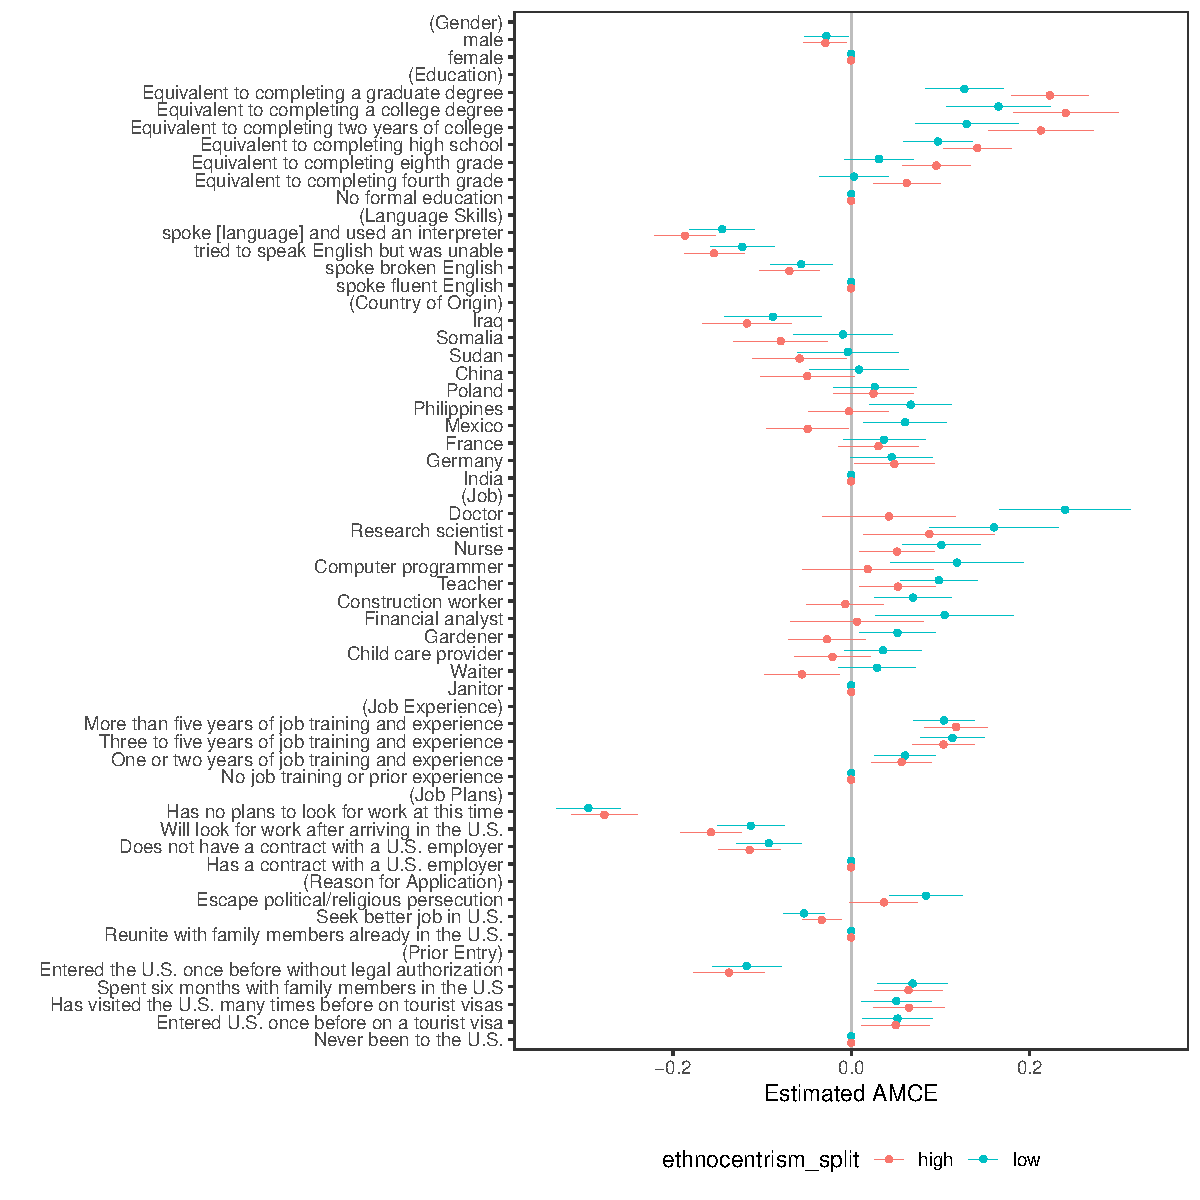
\includegraphics[width=\maxwidth]{figure/hainmueller_immigration_subgroup_amce_appendix-1} 

\end{knitrout}

\clearpage

\subsection{Subgroup Analysis for Hainmueller et al. (2014) Immigration Experiment using MMs}

\begin{knitrout}
\definecolor{shadecolor}{rgb}{0.969, 0.969, 0.969}\color{fgcolor}
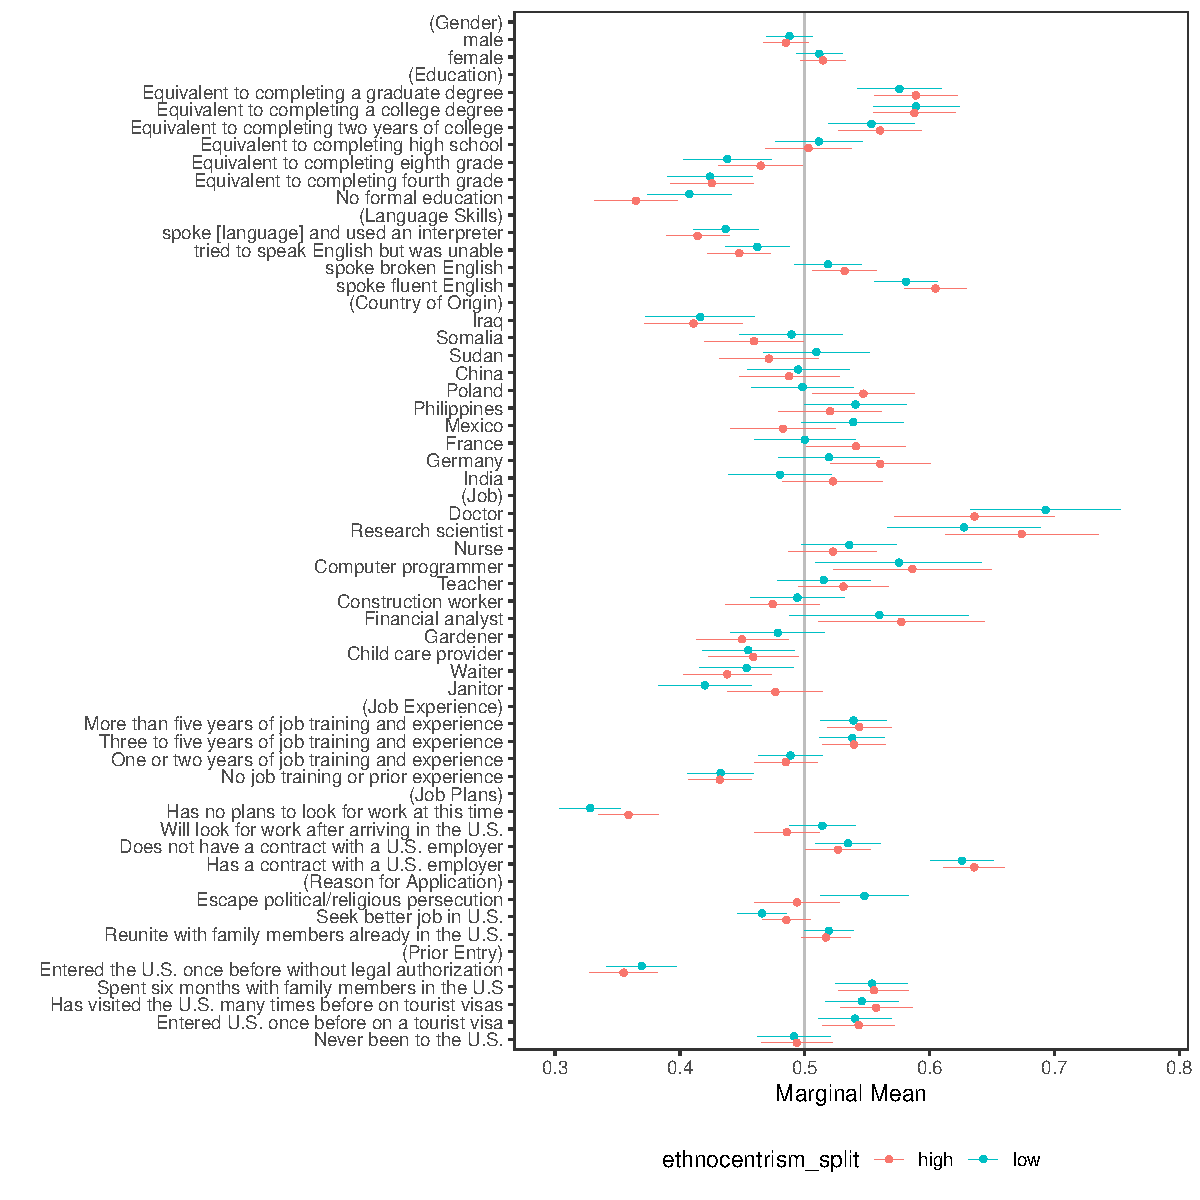
\includegraphics[width=\maxwidth]{figure/hainmueller_immigration_subgroup_mm_appendix-1} 

\end{knitrout}

\clearpage

\section{Hainmueller et al. (2014) Candidate Experiment}

\subsection{Replication using AMCEs}

\begin{knitrout}
\definecolor{shadecolor}{rgb}{0.969, 0.969, 0.969}\color{fgcolor}
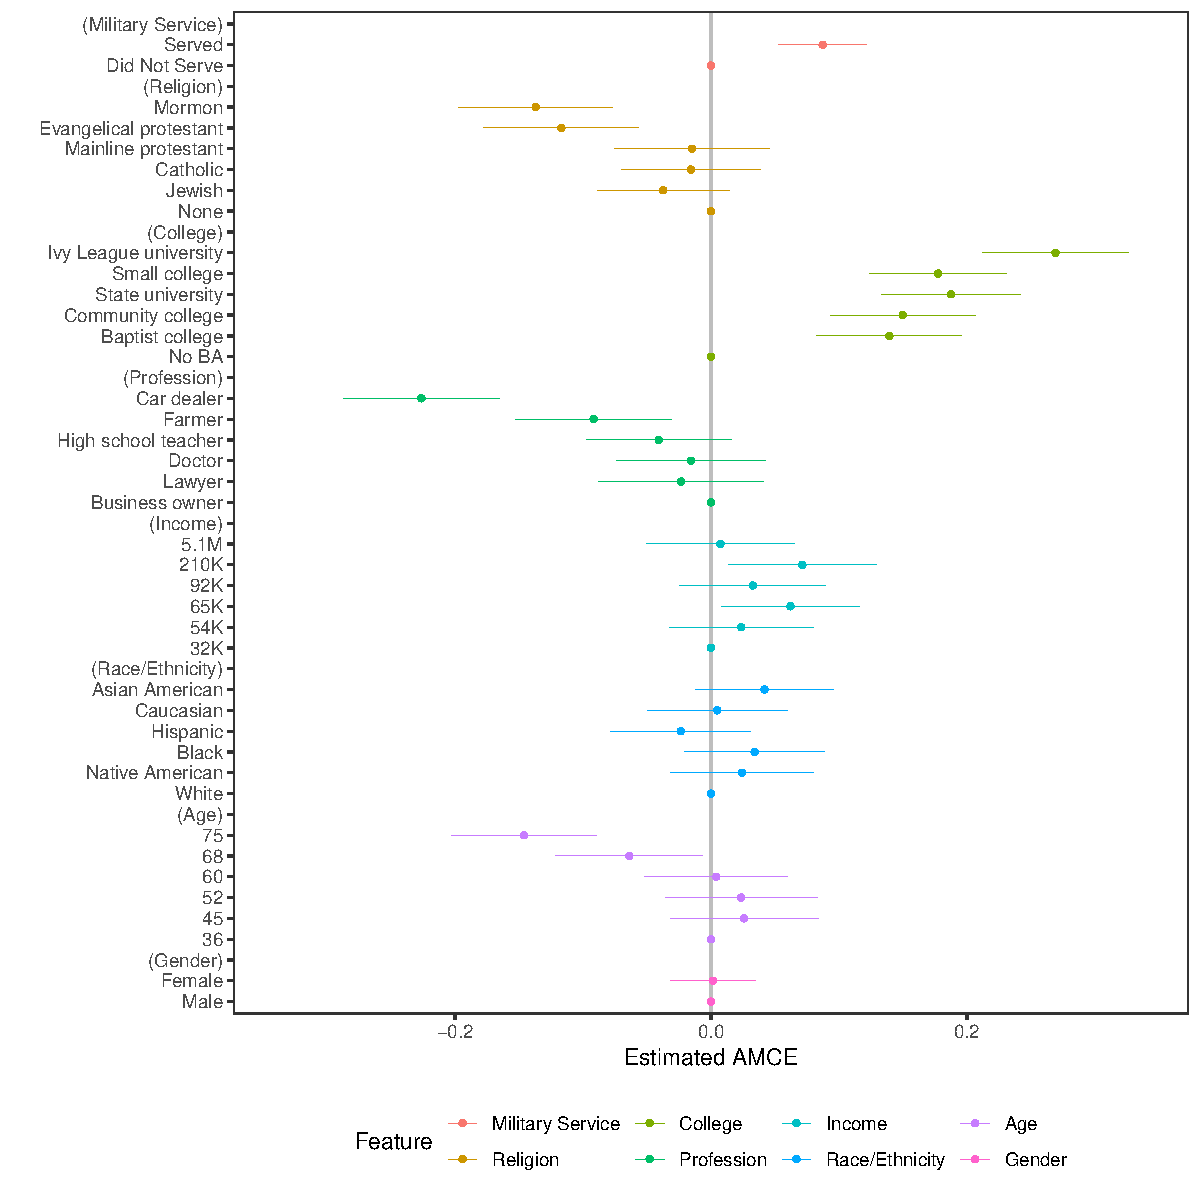
\includegraphics[width=\maxwidth]{figure/hainmueller_candidate_amce_appendix-1} 

\end{knitrout}

\clearpage

% latex table generated in R 3.5.1 by xtable 1.8-3 package
% Sun Nov 25 10:42:42 2018
\begin{table}[ht]
\centering
\begingroup\footnotesize
\begin{tabular}{lp{3in}rrr}
  \hline
feature & level & estimate & std.error & z \\ 
  \hline
Military Service & Did Not Serve & 0.00 &  &  \\ 
  Military Service & Served & 0.09 & 0.02 & 4.95 \\ 
  Religion & None & 0.00 &  &  \\ 
  Religion & Jewish & -0.04 & 0.03 & -1.42 \\ 
  Religion & Catholic & -0.02 & 0.03 & -0.56 \\ 
  Religion & Mainline protestant & -0.01 & 0.03 & -0.48 \\ 
  Religion & Evangelical protestant & -0.12 & 0.03 & -3.78 \\ 
  Religion & Mormon & -0.14 & 0.03 & -4.46 \\ 
  College & No BA & 0.00 &  &  \\ 
  College & Baptist college & 0.14 & 0.03 & 4.82 \\ 
  College & Community college & 0.15 & 0.03 & 5.17 \\ 
  College & State university & 0.19 & 0.03 & 6.77 \\ 
  College & Small college & 0.18 & 0.03 & 6.50 \\ 
  College & Ivy League university & 0.27 & 0.03 & 9.26 \\ 
  Profession & Business owner & 0.00 &  &  \\ 
  Profession & Lawyer & -0.02 & 0.03 & -0.71 \\ 
  Profession & Doctor & -0.02 & 0.03 & -0.53 \\ 
  Profession & High school teacher & -0.04 & 0.03 & -1.42 \\ 
  Profession & Farmer & -0.09 & 0.03 & -2.94 \\ 
  Profession & Car dealer & -0.23 & 0.03 & -7.24 \\ 
  Income & 32K & 0.00 &  &  \\ 
  Income & 54K & 0.02 & 0.03 & 0.82 \\ 
  Income & 65K & 0.06 & 0.03 & 2.26 \\ 
  Income & 92K & 0.03 & 0.03 & 1.12 \\ 
  Income & 210K & 0.07 & 0.03 & 2.41 \\ 
  Income & 5.1M & 0.01 & 0.03 & 0.25 \\ 
  Race/Ethnicity & White & 0.00 &  &  \\ 
  Race/Ethnicity & Native American & 0.02 & 0.03 & 0.85 \\ 
  Race/Ethnicity & Black & 0.03 & 0.03 & 1.22 \\ 
  Race/Ethnicity & Hispanic & -0.02 & 0.03 & -0.84 \\ 
  Race/Ethnicity & Caucasian & 0.00 & 0.03 & 0.18 \\ 
  Race/Ethnicity & Asian American & 0.04 & 0.03 & 1.51 \\ 
  Age & 36 & 0.00 &  &  \\ 
  Age & 45 & 0.03 & 0.03 & 0.88 \\ 
  Age & 52 & 0.02 & 0.03 & 0.78 \\ 
  Age & 60 & 0.00 & 0.03 & 0.14 \\ 
  Age & 68 & -0.06 & 0.03 & -2.17 \\ 
  Age & 75 & -0.15 & 0.03 & -5.06 \\ 
  Gender & Male & 0.00 &  &  \\ 
  Gender & Female & 0.00 & 0.02 & 0.09 \\ 
   \hline
\end{tabular}
\endgroup
\end{table}


\clearpage

\subsection{Replication using MMs}

\begin{knitrout}
\definecolor{shadecolor}{rgb}{0.969, 0.969, 0.969}\color{fgcolor}
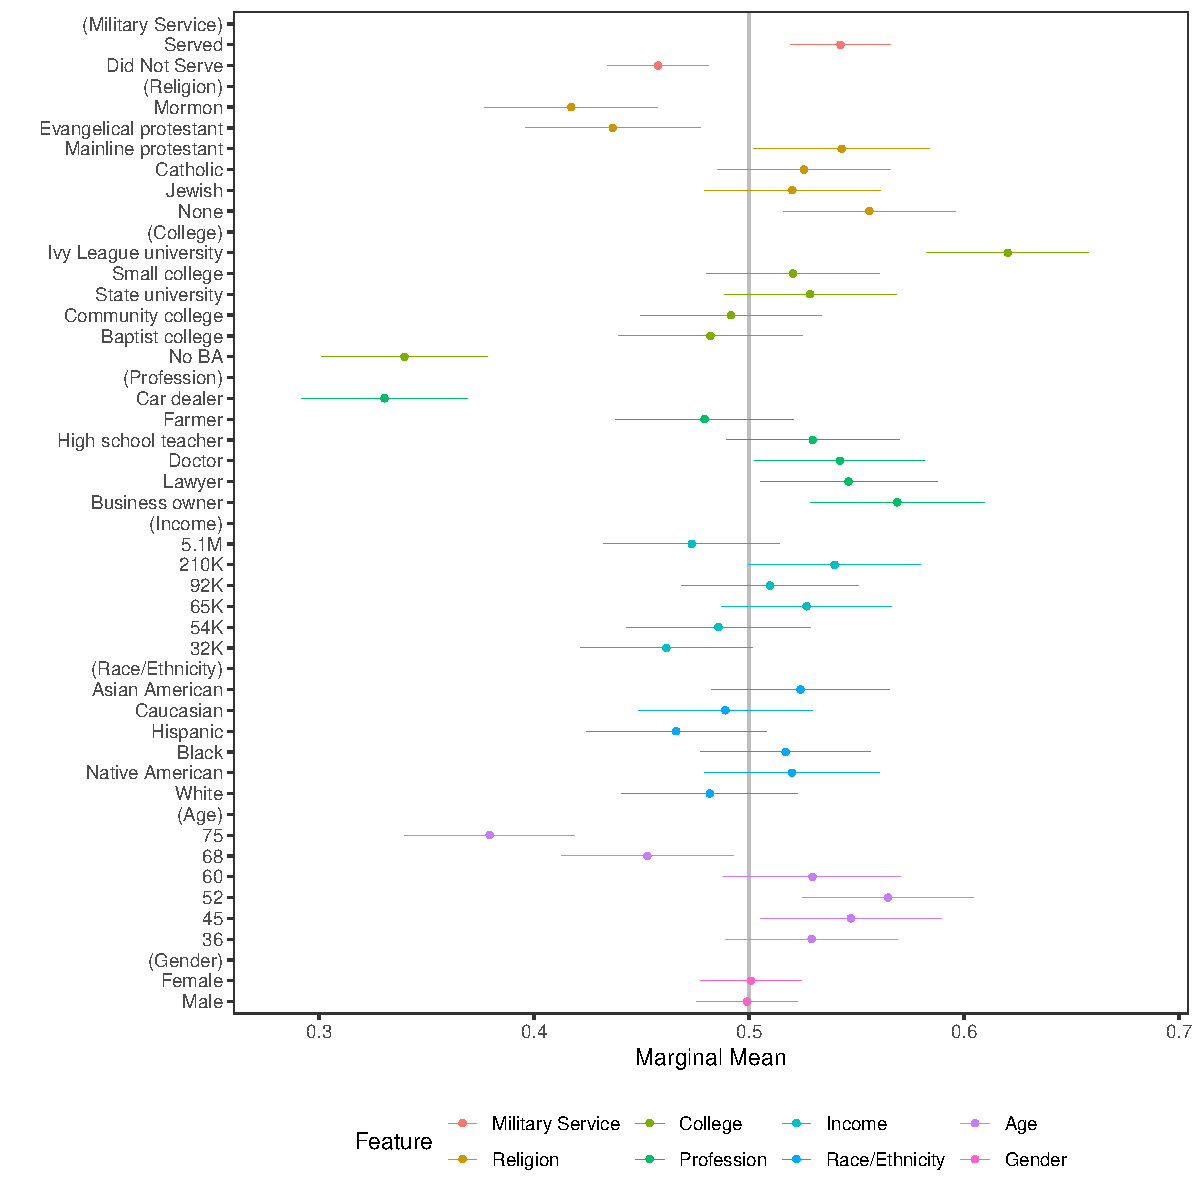
\includegraphics[width=\maxwidth]{figure/hainmueller_candidate_mm_appendix-1} 

\end{knitrout}

\clearpage

% latex table generated in R 3.5.1 by xtable 1.8-3 package
% Sun Nov 25 10:42:44 2018
\begin{table}[ht]
\centering
\begingroup\footnotesize
\begin{tabular}{lp{3in}rrr}
  \hline
feature & level & estimate & std.error & z \\ 
  \hline
Military Service & Did Not Serve & 0.46 & 0.01 & -3.54 \\ 
  Military Service & Served & 0.54 & 0.01 & 3.55 \\ 
  Religion & None & 0.56 & 0.02 & 2.73 \\ 
  Religion & Jewish & 0.52 & 0.02 & 0.96 \\ 
  Religion & Catholic & 0.53 & 0.02 & 1.24 \\ 
  Religion & Mainline protestant & 0.54 & 0.02 & 2.06 \\ 
  Religion & Evangelical protestant & 0.44 & 0.02 & -3.05 \\ 
  Religion & Mormon & 0.42 & 0.02 & -4.04 \\ 
  College & No BA & 0.34 & 0.02 & -8.11 \\ 
  College & Baptist college & 0.48 & 0.02 & -0.83 \\ 
  College & Community college & 0.49 & 0.02 & -0.39 \\ 
  College & State university & 0.53 & 0.02 & 1.39 \\ 
  College & Small college & 0.52 & 0.02 & 0.99 \\ 
  College & Ivy League university & 0.62 & 0.02 & 6.27 \\ 
  Profession & Business owner & 0.57 & 0.02 & 3.35 \\ 
  Profession & Lawyer & 0.55 & 0.02 & 2.20 \\ 
  Profession & Doctor & 0.54 & 0.02 & 2.08 \\ 
  Profession & High school teacher & 0.53 & 0.02 & 1.44 \\ 
  Profession & Farmer & 0.48 & 0.02 & -0.98 \\ 
  Profession & Car dealer & 0.33 & 0.02 & -8.64 \\ 
  Income & 32K & 0.46 & 0.02 & -1.89 \\ 
  Income & 54K & 0.49 & 0.02 & -0.65 \\ 
  Income & 65K & 0.53 & 0.02 & 1.33 \\ 
  Income & 92K & 0.51 & 0.02 & 0.46 \\ 
  Income & 210K & 0.54 & 0.02 & 1.94 \\ 
  Income & 5.1M & 0.47 & 0.02 & -1.26 \\ 
  Race/Ethnicity & White & 0.48 & 0.02 & -0.88 \\ 
  Race/Ethnicity & Native American & 0.52 & 0.02 & 0.96 \\ 
  Race/Ethnicity & Black & 0.52 & 0.02 & 0.85 \\ 
  Race/Ethnicity & Hispanic & 0.47 & 0.02 & -1.59 \\ 
  Race/Ethnicity & Caucasian & 0.49 & 0.02 & -0.53 \\ 
  Race/Ethnicity & Asian American & 0.52 & 0.02 & 1.14 \\ 
  Age & 36 & 0.53 & 0.02 & 1.43 \\ 
  Age & 45 & 0.55 & 0.02 & 2.21 \\ 
  Age & 52 & 0.56 & 0.02 & 3.18 \\ 
  Age & 60 & 0.53 & 0.02 & 1.40 \\ 
  Age & 68 & 0.45 & 0.02 & -2.31 \\ 
  Age & 75 & 0.38 & 0.02 & -5.99 \\ 
  Gender & Male & 0.50 & 0.01 & -0.07 \\ 
  Gender & Female & 0.50 & 0.01 & 0.07 \\ 
   \hline
\end{tabular}
\endgroup
\end{table}


\clearpage

\section{Ballard-Rosa et al. (2016) Tax Preference Experiment}

\subsection{Replication using AMCEs}

\begin{knitrout}
\definecolor{shadecolor}{rgb}{0.969, 0.969, 0.969}\color{fgcolor}
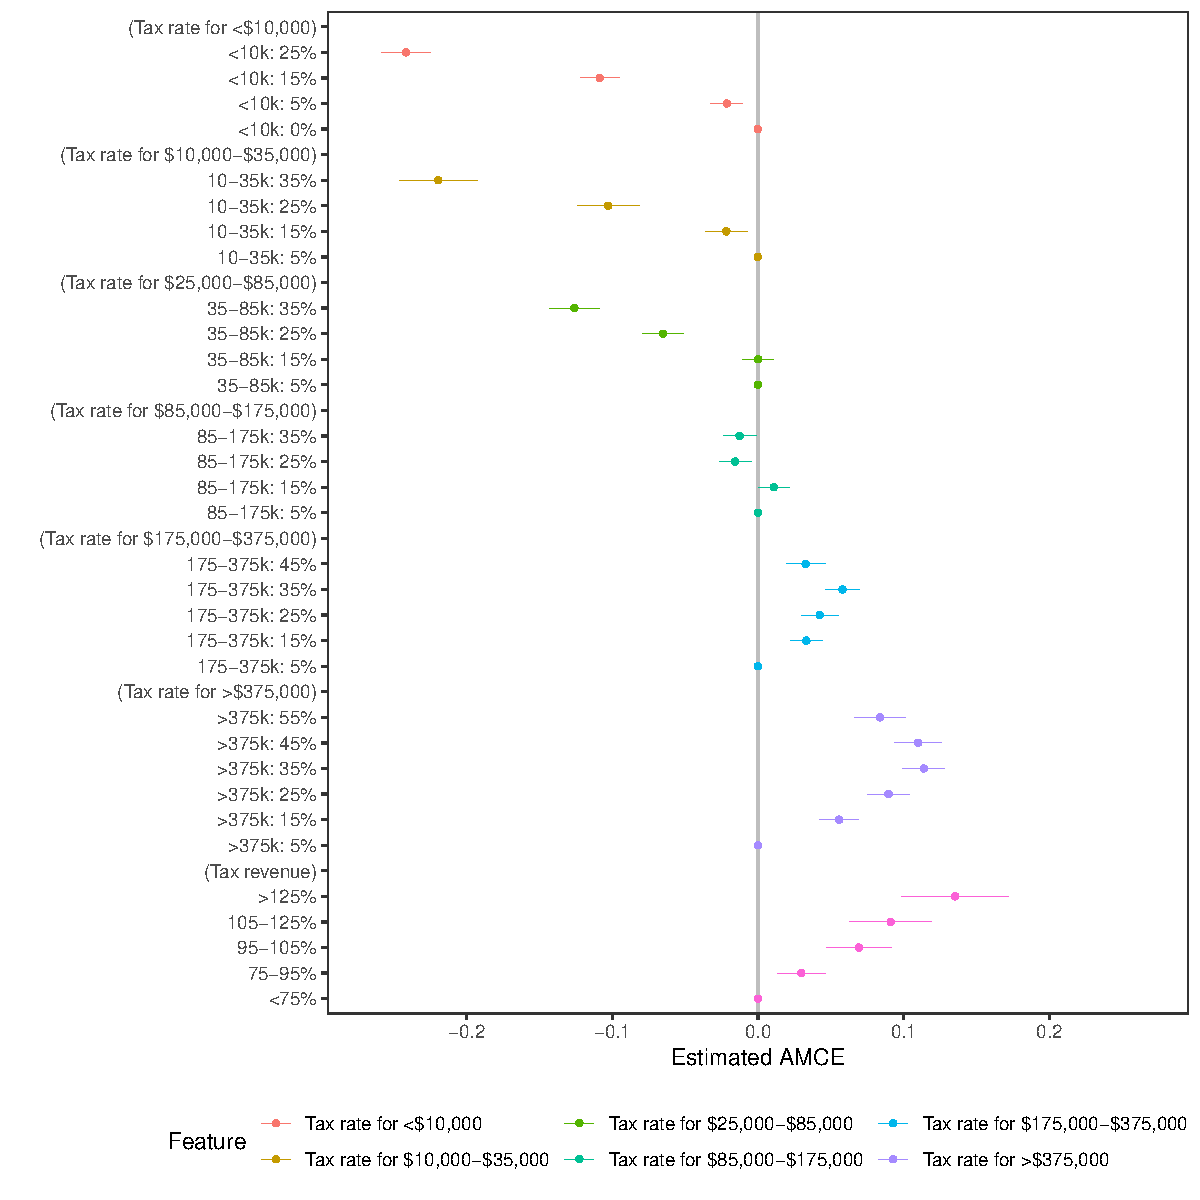
\includegraphics[width=\maxwidth]{figure/bms_amce_appendix-1} 

\end{knitrout}

\clearpage

% latex table generated in R 3.5.1 by xtable 1.8-3 package
% Sun Nov 25 10:42:47 2018
\begin{table}[ht]
\centering
\begin{tabular}{lp{1.5in}rrr}
  \hline
feature & level & estimate & std.error & z \\ 
  \hline
Tax rate for $<$\$10,000 & $<$10k: 0\% & 0.00 &  &  \\ 
  Tax rate for $<$\$10,000 & $<$10k: 5\% & -0.02 & 0.01 & -3.81 \\ 
  Tax rate for $<$\$10,000 & $<$10k: 15\% & -0.11 & 0.01 & -15.97 \\ 
  Tax rate for $<$\$10,000 & $<$10k: 25\% & -0.24 & 0.01 & -28.33 \\ 
  Tax rate for \$10,000-\$35,000 & 10-35k: 5\% & 0.00 &  &  \\ 
  Tax rate for \$10,000-\$35,000 & 10-35k: 15\% & -0.02 & 0.01 & -2.94 \\ 
  Tax rate for \$10,000-\$35,000 & 10-35k: 25\% & -0.10 & 0.01 & -9.42 \\ 
  Tax rate for \$10,000-\$35,000 & 10-35k: 35\% & -0.22 & 0.01 & -15.96 \\ 
  Tax rate for \$25,000-\$85,000 & 35-85k: 5\% & 0.00 &  &  \\ 
  Tax rate for \$25,000-\$85,000 & 35-85k: 15\% & 0.00 & 0.01 & 0.03 \\ 
  Tax rate for \$25,000-\$85,000 & 35-85k: 25\% & -0.07 & 0.01 & -9.18 \\ 
  Tax rate for \$25,000-\$85,000 & 35-85k: 35\% & -0.13 & 0.01 & -14.55 \\ 
  Tax rate for \$85,000-\$175,000 & 85-175k: 5\% & 0.00 &  &  \\ 
  Tax rate for \$85,000-\$175,000 & 85-175k: 15\% & 0.01 & 0.01 & 2.06 \\ 
  Tax rate for \$85,000-\$175,000 & 85-175k: 25\% & -0.02 & 0.01 & -2.80 \\ 
  Tax rate for \$85,000-\$175,000 & 85-175k: 35\% & -0.01 & 0.01 & -2.19 \\ 
  Tax rate for \$175,000-\$375,000 & 175-375k: 5\% & 0.00 &  &  \\ 
  Tax rate for \$175,000-\$375,000 & 175-375k: 15\% & 0.03 & 0.01 & 5.97 \\ 
  Tax rate for \$175,000-\$375,000 & 175-375k: 25\% & 0.04 & 0.01 & 6.53 \\ 
  Tax rate for \$175,000-\$375,000 & 175-375k: 35\% & 0.06 & 0.01 & 9.77 \\ 
  Tax rate for \$175,000-\$375,000 & 175-375k: 45\% & 0.03 & 0.01 & 4.80 \\ 
  Tax rate for $>$\$375,000 & $>$375k: 5\% & 0.00 &  &  \\ 
  Tax rate for $>$\$375,000 & $>$375k: 15\% & 0.06 & 0.01 & 8.22 \\ 
  Tax rate for $>$\$375,000 & $>$375k: 25\% & 0.09 & 0.01 & 12.18 \\ 
  Tax rate for $>$\$375,000 & $>$375k: 35\% & 0.11 & 0.01 & 15.44 \\ 
  Tax rate for $>$\$375,000 & $>$375k: 45\% & 0.11 & 0.01 & 13.23 \\ 
  Tax rate for $>$\$375,000 & $>$375k: 55\% & 0.08 & 0.01 & 9.55 \\ 
  Tax revenue & $<$75\% & 0.00 &  &  \\ 
  Tax revenue & 75-95\% & 0.03 & 0.01 & 3.56 \\ 
  Tax revenue & 95-105\% & 0.07 & 0.01 & 6.11 \\ 
  Tax revenue & 105-125\% & 0.09 & 0.01 & 6.33 \\ 
  Tax revenue & $>$125\% & 0.14 & 0.02 & 7.22 \\ 
   \hline
\end{tabular}
\end{table}


\clearpage

\subsection{Replication using MMs}

\begin{knitrout}
\definecolor{shadecolor}{rgb}{0.969, 0.969, 0.969}\color{fgcolor}
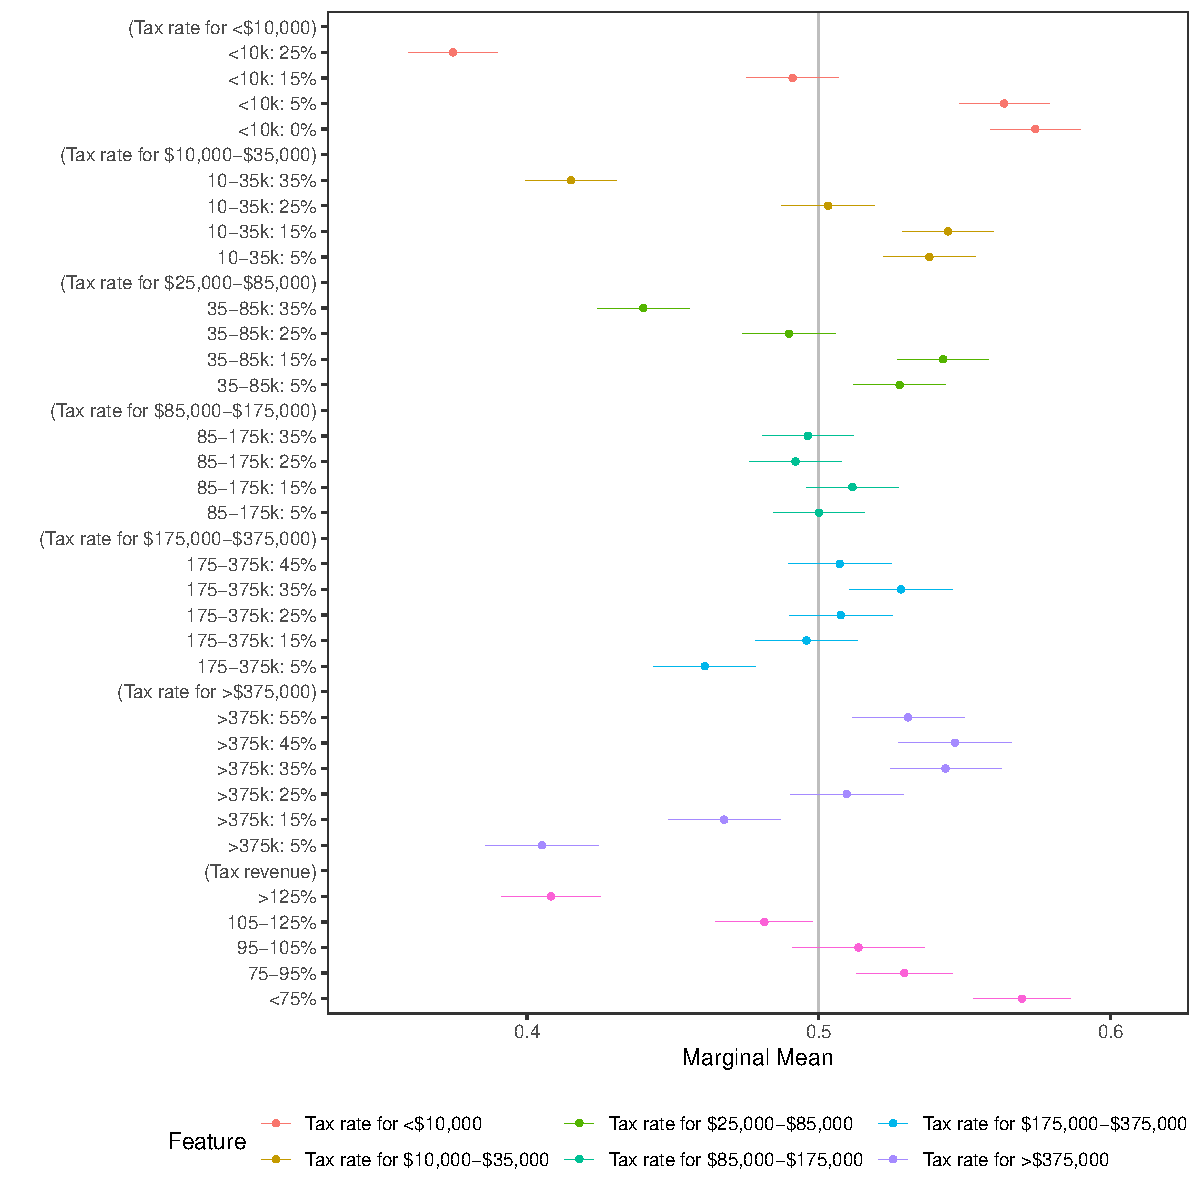
\includegraphics[width=\maxwidth]{figure/bms_mm_appendix-1} 

\end{knitrout}

\clearpage

% latex table generated in R 3.5.1 by xtable 1.8-3 package
% Sun Nov 25 10:42:56 2018
\begin{table}[ht]
\centering
\begin{tabular}{lp{1.5in}rrr}
  \hline
feature & level & estimate & std.error & z \\ 
  \hline
Tax rate for $<$\$10,000 & $<$10k: 0\% & 0.57 & 0.01 & 9.37 \\ 
  Tax rate for $<$\$10,000 & $<$10k: 5\% & 0.56 & 0.01 & 8.06 \\ 
  Tax rate for $<$\$10,000 & $<$10k: 15\% & 0.49 & 0.01 & -1.11 \\ 
  Tax rate for $<$\$10,000 & $<$10k: 25\% & 0.37 & 0.01 & -16.07 \\ 
  Tax rate for \$10,000-\$35,000 & 10-35k: 5\% & 0.54 & 0.01 & 4.75 \\ 
  Tax rate for \$10,000-\$35,000 & 10-35k: 15\% & 0.54 & 0.01 & 5.55 \\ 
  Tax rate for \$10,000-\$35,000 & 10-35k: 25\% & 0.50 & 0.01 & 0.39 \\ 
  Tax rate for \$10,000-\$35,000 & 10-35k: 35\% & 0.42 & 0.01 & -10.62 \\ 
  Tax rate for \$25,000-\$85,000 & 35-85k: 5\% & 0.53 & 0.01 & 3.45 \\ 
  Tax rate for \$25,000-\$85,000 & 35-85k: 15\% & 0.54 & 0.01 & 5.37 \\ 
  Tax rate for \$25,000-\$85,000 & 35-85k: 25\% & 0.49 & 0.01 & -1.27 \\ 
  Tax rate for \$25,000-\$85,000 & 35-85k: 35\% & 0.44 & 0.01 & -7.50 \\ 
  Tax rate for \$85,000-\$175,000 & 85-175k: 5\% & 0.50 & 0.01 & 0.00 \\ 
  Tax rate for \$85,000-\$175,000 & 85-175k: 15\% & 0.51 & 0.01 & 1.42 \\ 
  Tax rate for \$85,000-\$175,000 & 85-175k: 25\% & 0.49 & 0.01 & -1.00 \\ 
  Tax rate for \$85,000-\$175,000 & 85-175k: 35\% & 0.50 & 0.01 & -0.46 \\ 
  Tax rate for \$175,000-\$375,000 & 175-375k: 5\% & 0.46 & 0.01 & -4.37 \\ 
  Tax rate for \$175,000-\$375,000 & 175-375k: 15\% & 0.50 & 0.01 & -0.47 \\ 
  Tax rate for \$175,000-\$375,000 & 175-375k: 25\% & 0.51 & 0.01 & 0.84 \\ 
  Tax rate for \$175,000-\$375,000 & 175-375k: 35\% & 0.53 & 0.01 & 3.11 \\ 
  Tax rate for \$175,000-\$375,000 & 175-375k: 45\% & 0.51 & 0.01 & 0.80 \\ 
  Tax rate for $>$\$375,000 & $>$375k: 5\% & 0.41 & 0.01 & -9.57 \\ 
  Tax rate for $>$\$375,000 & $>$375k: 15\% & 0.47 & 0.01 & -3.30 \\ 
  Tax rate for $>$\$375,000 & $>$375k: 25\% & 0.51 & 0.01 & 0.97 \\ 
  Tax rate for $>$\$375,000 & $>$375k: 35\% & 0.54 & 0.01 & 4.48 \\ 
  Tax rate for $>$\$375,000 & $>$375k: 45\% & 0.55 & 0.01 & 4.75 \\ 
  Tax rate for $>$\$375,000 & $>$375k: 55\% & 0.53 & 0.01 & 3.12 \\ 
  Tax revenue & $<$75\% & 0.57 & 0.01 & 8.22 \\ 
  Tax revenue & 75-95\% & 0.53 & 0.01 & 3.47 \\ 
  Tax revenue & 95-105\% & 0.51 & 0.01 & 1.18 \\ 
  Tax revenue & 105-125\% & 0.48 & 0.01 & -2.21 \\ 
  Tax revenue & $>$125\% & 0.41 & 0.01 & -10.54 \\ 
   \hline
\end{tabular}
\end{table}


\clearpage

\subsection{Subgroup Analysis for Ballard-Rosa et al. (2016), by ``Taxes Harm Economy'' Split using AMCEs}

\begin{knitrout}
\definecolor{shadecolor}{rgb}{0.969, 0.969, 0.969}\color{fgcolor}
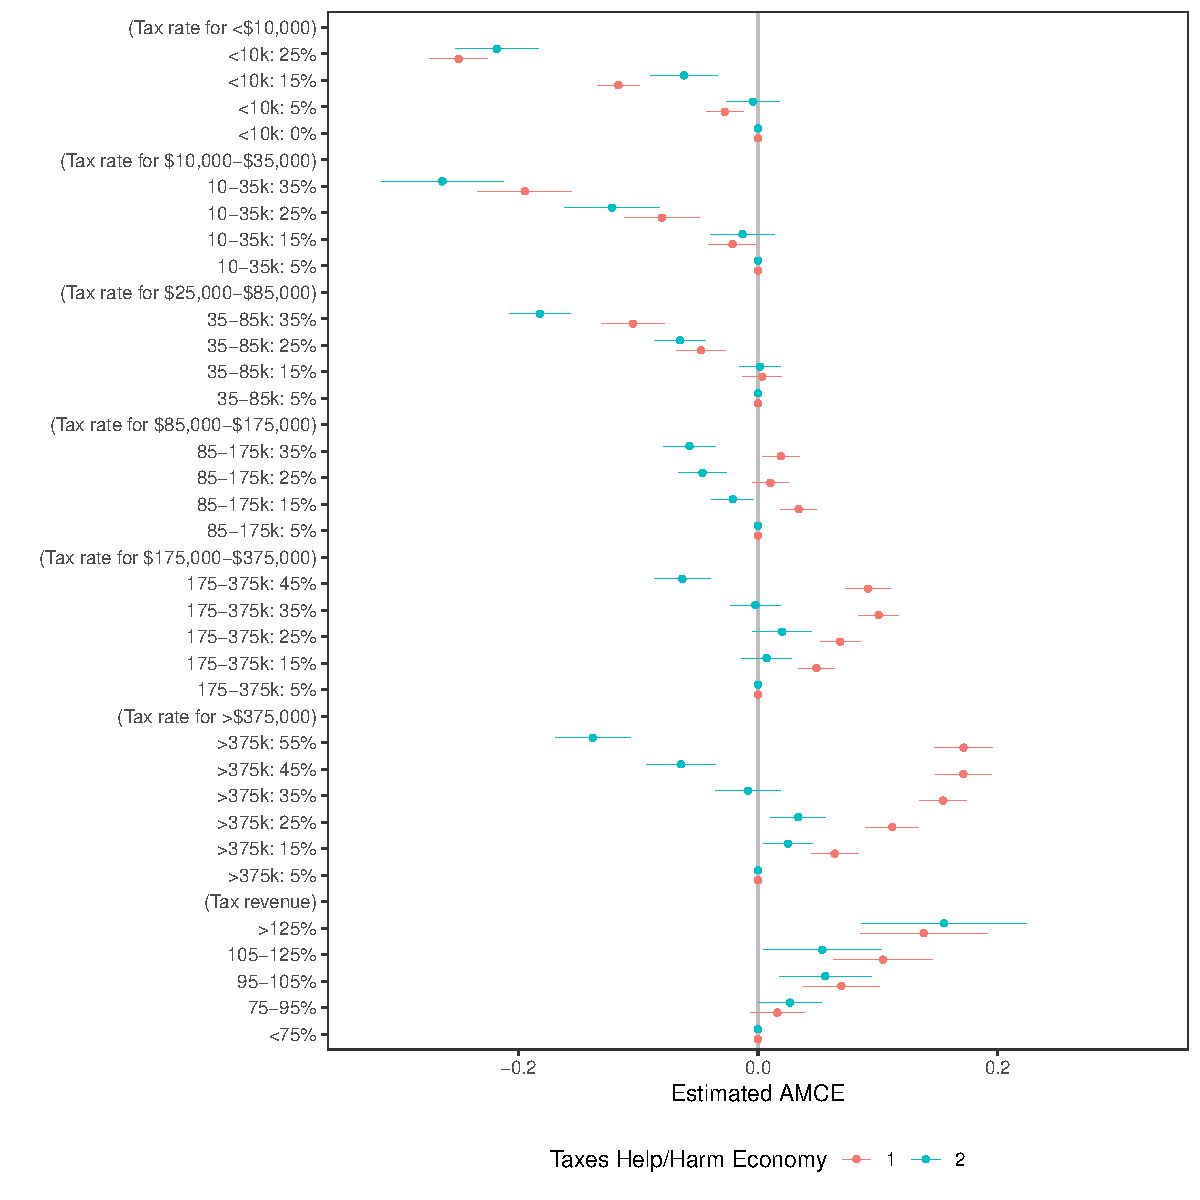
\includegraphics[width=\maxwidth]{figure/bms_subgroup_amce_appendix1-1} 

\end{knitrout}

\clearpage

\subsection{Subgroup Analysis for Ballard-Rosa et al. (2016), by ``Taxes Harm Economy'' Split using MMs}

\begin{knitrout}
\definecolor{shadecolor}{rgb}{0.969, 0.969, 0.969}\color{fgcolor}
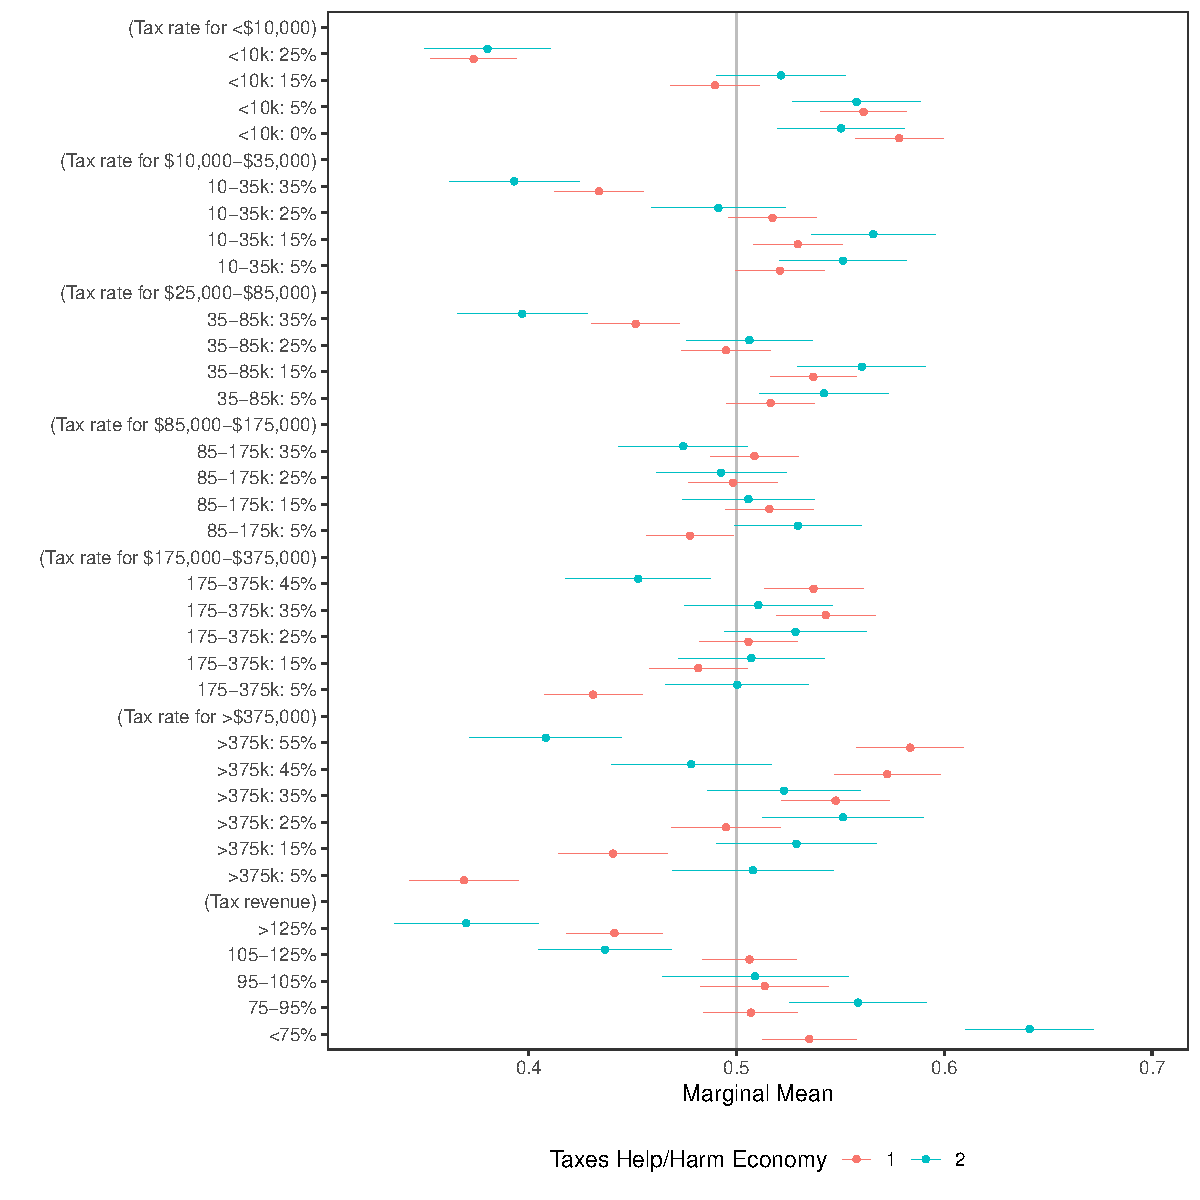
\includegraphics[width=\maxwidth]{figure/bms_subgroup_mm_appendix1-1} 

\end{knitrout}

\clearpage

\subsection{Subgroup Analysis for Ballard-Rosa et al. (2016), by Inequity Aversion using AMCEs}

\begin{knitrout}
\definecolor{shadecolor}{rgb}{0.969, 0.969, 0.969}\color{fgcolor}
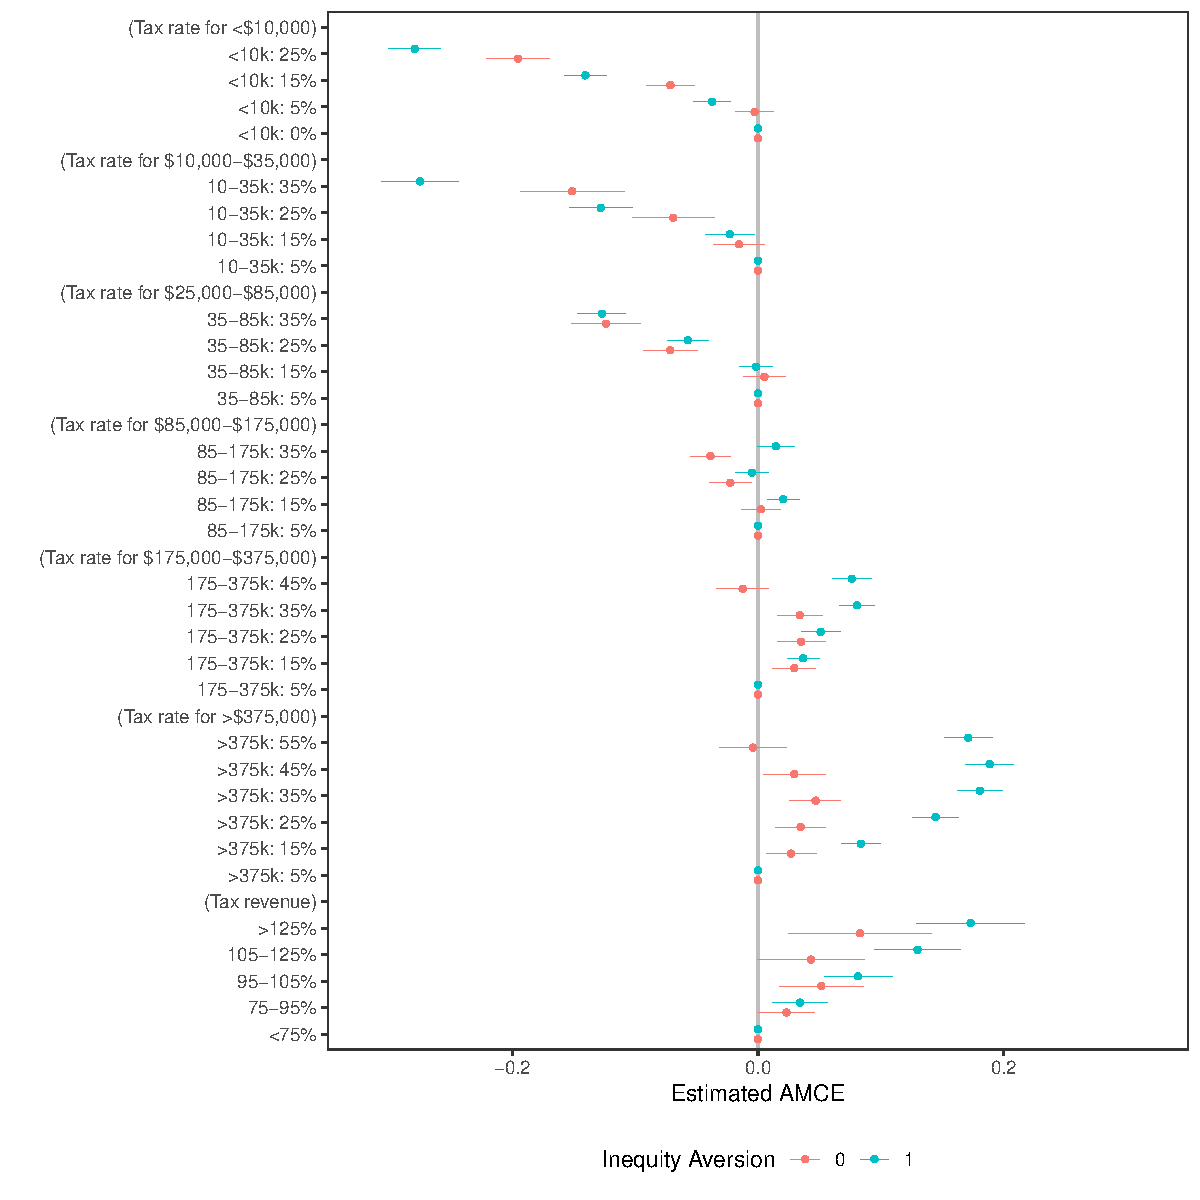
\includegraphics[width=\maxwidth]{figure/bms_subgroup_amce_appendix2-1} 

\end{knitrout}

\clearpage

\subsection{Subgroup Analysis for Ballard-Rosa et al. (2016), by Inequity Aversion using MMs}

\begin{knitrout}
\definecolor{shadecolor}{rgb}{0.969, 0.969, 0.969}\color{fgcolor}
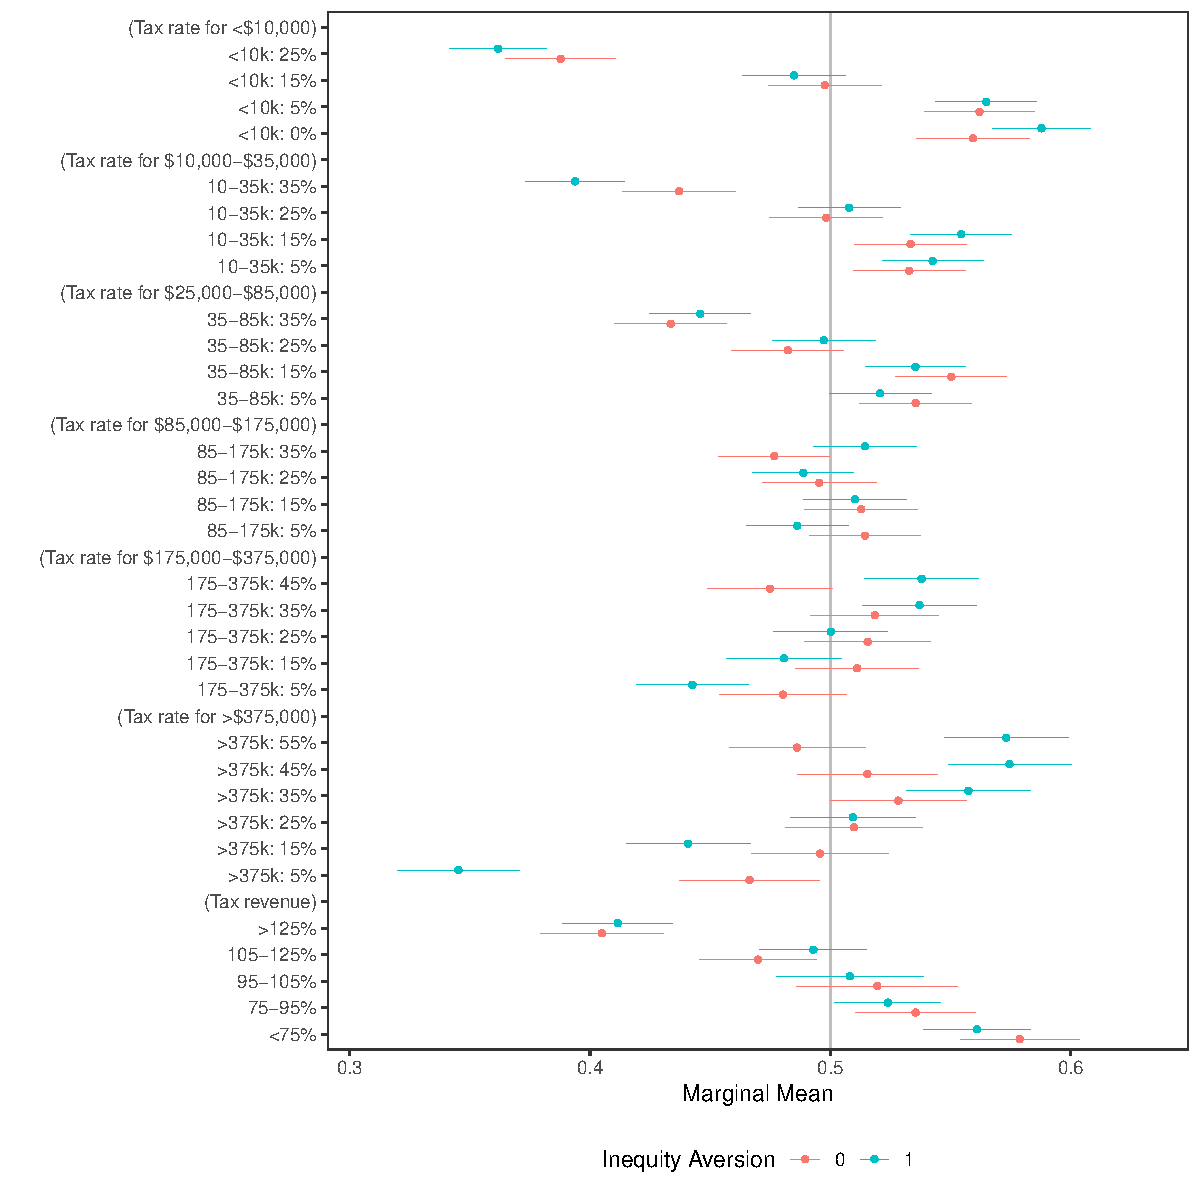
\includegraphics[width=\maxwidth]{figure/bms_subgroup_mm_appendix2-1} 

\end{knitrout}

\clearpage

\subsection{Comparison of Alternative Reference Categories for Ballard-Rosa et al. (2016) Tax Preference Experiment, by ``Taxes Harm Economy'' Split}



\begin{knitrout}
\definecolor{shadecolor}{rgb}{0.969, 0.969, 0.969}\color{fgcolor}
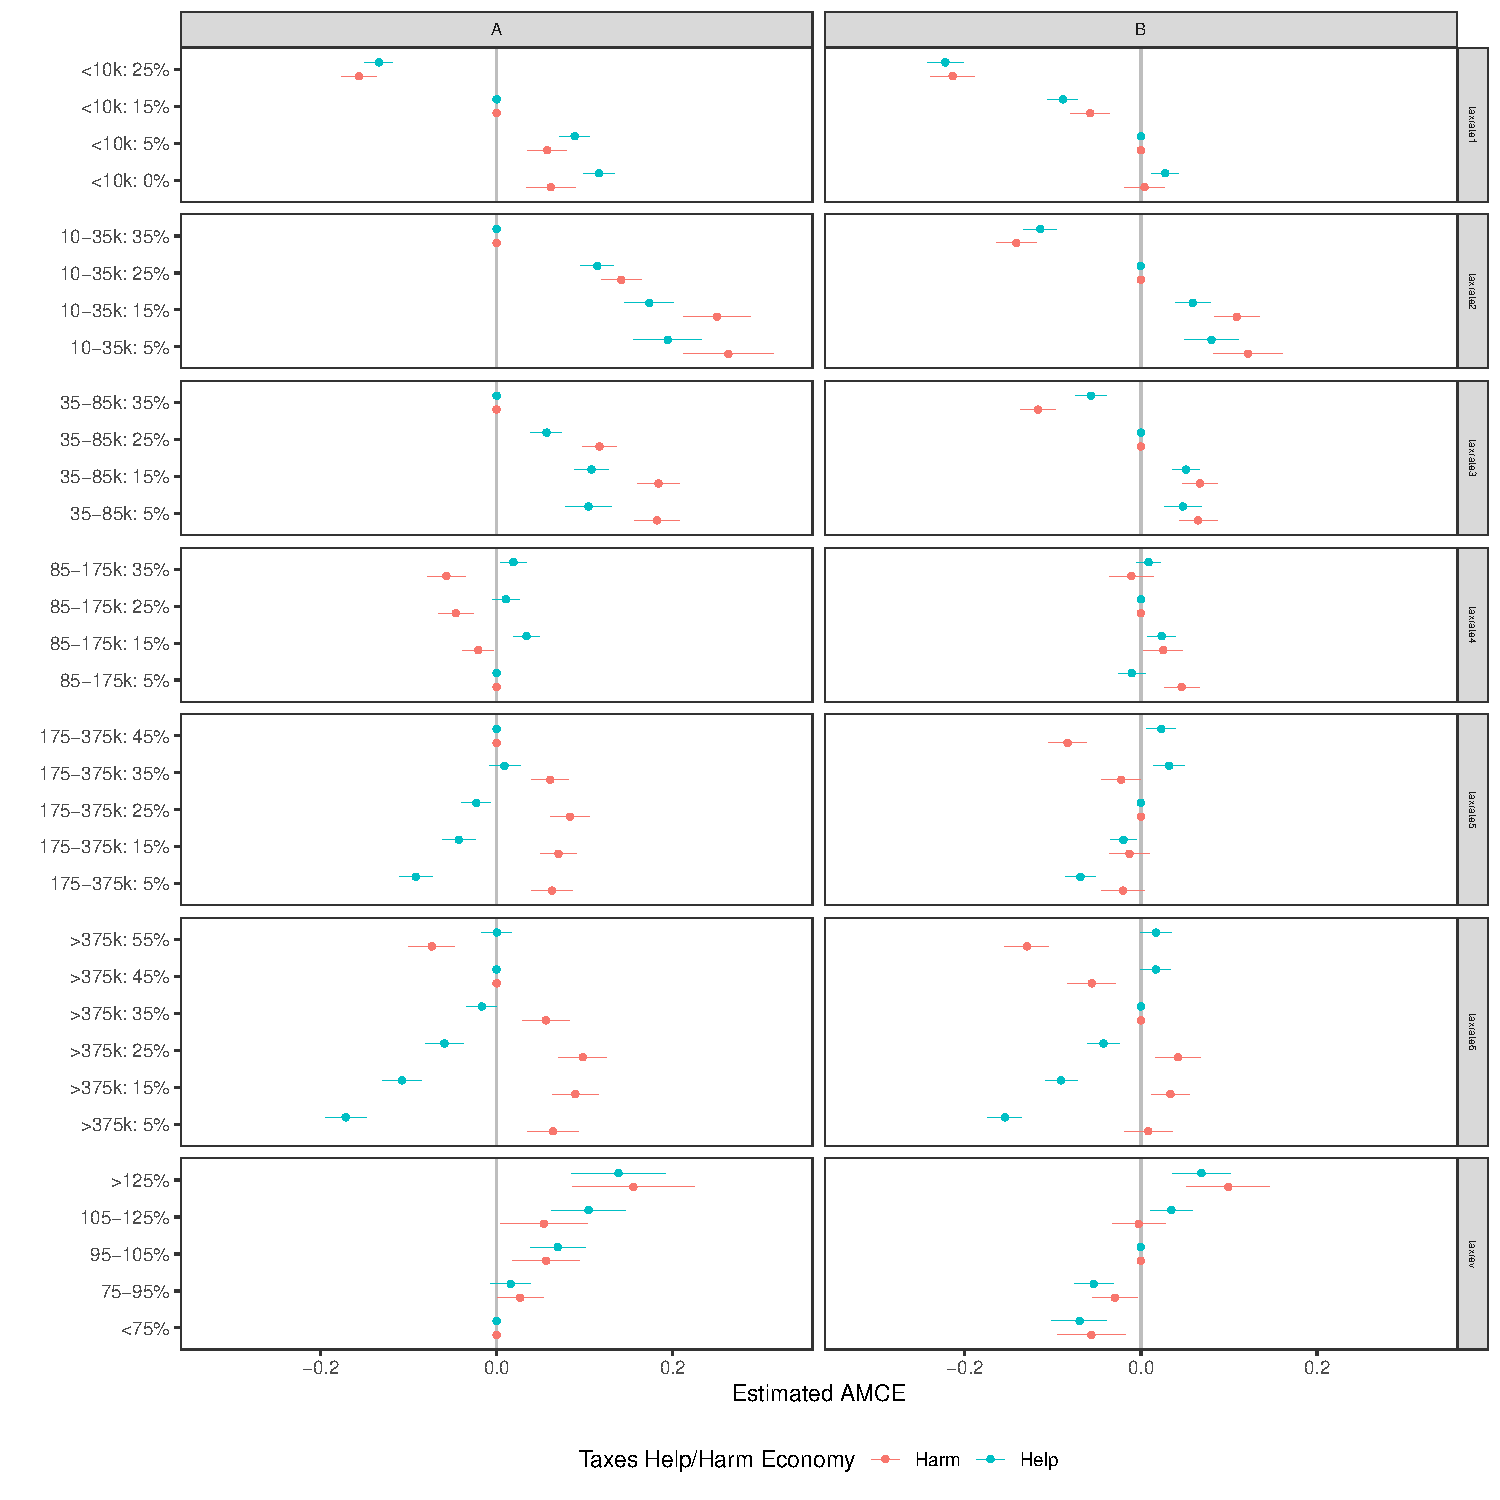
\includegraphics[width=\maxwidth]{figure/bms_subgroup_example_plot1-1} 

\end{knitrout}

\clearpage

\subsection{Comparison of Alternative Reference Categories for Ballard-Rosa et al. (2016) Tax Preference Experiment, by Inequity Aversion}



\begin{knitrout}
\definecolor{shadecolor}{rgb}{0.969, 0.969, 0.969}\color{fgcolor}
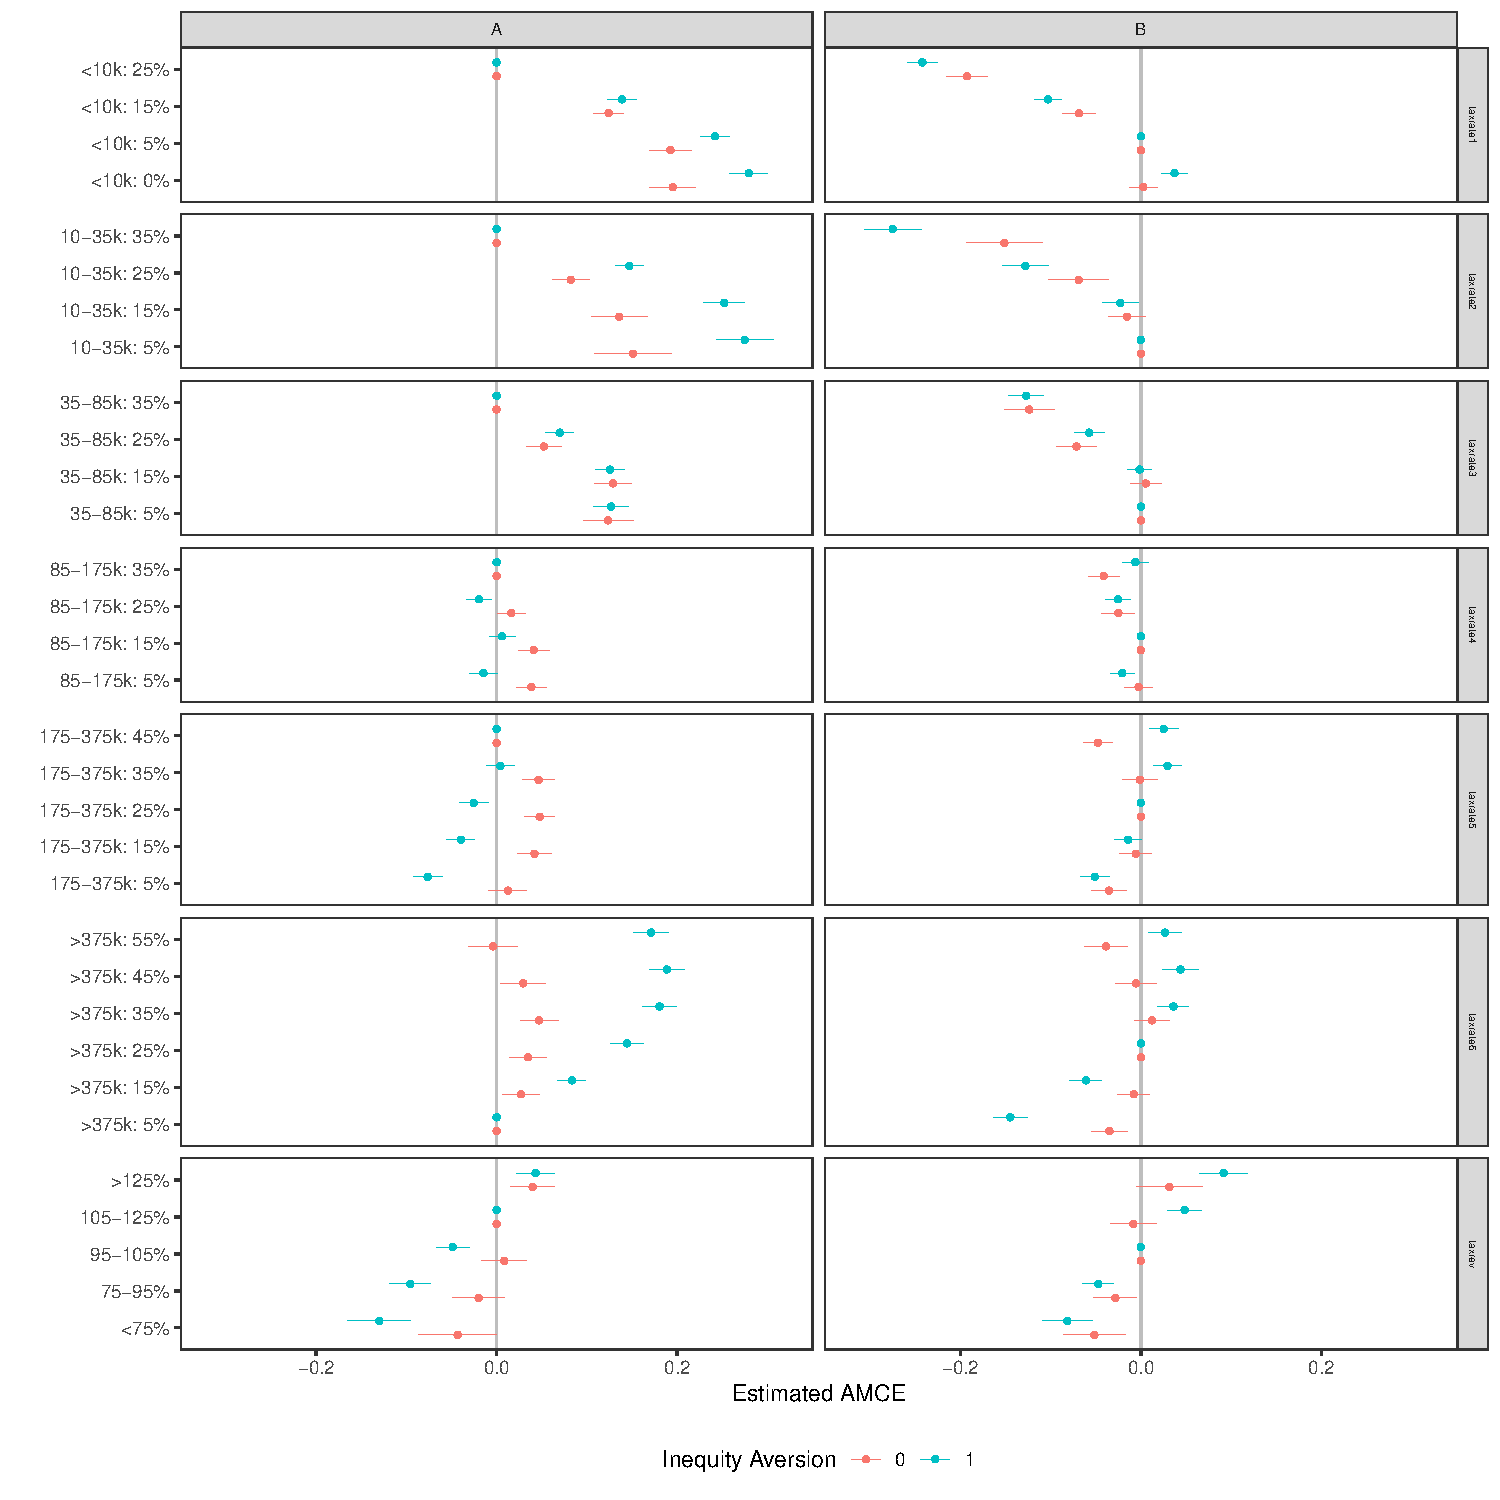
\includegraphics[width=\maxwidth]{figure/bms_subgroup_example_plot2-1} 

\end{knitrout}

\clearpage

\section{Teele et al. (2018) Candidate Experiment}

\subsection{Replication using AMCEs}

\begin{knitrout}
\definecolor{shadecolor}{rgb}{0.969, 0.969, 0.969}\color{fgcolor}
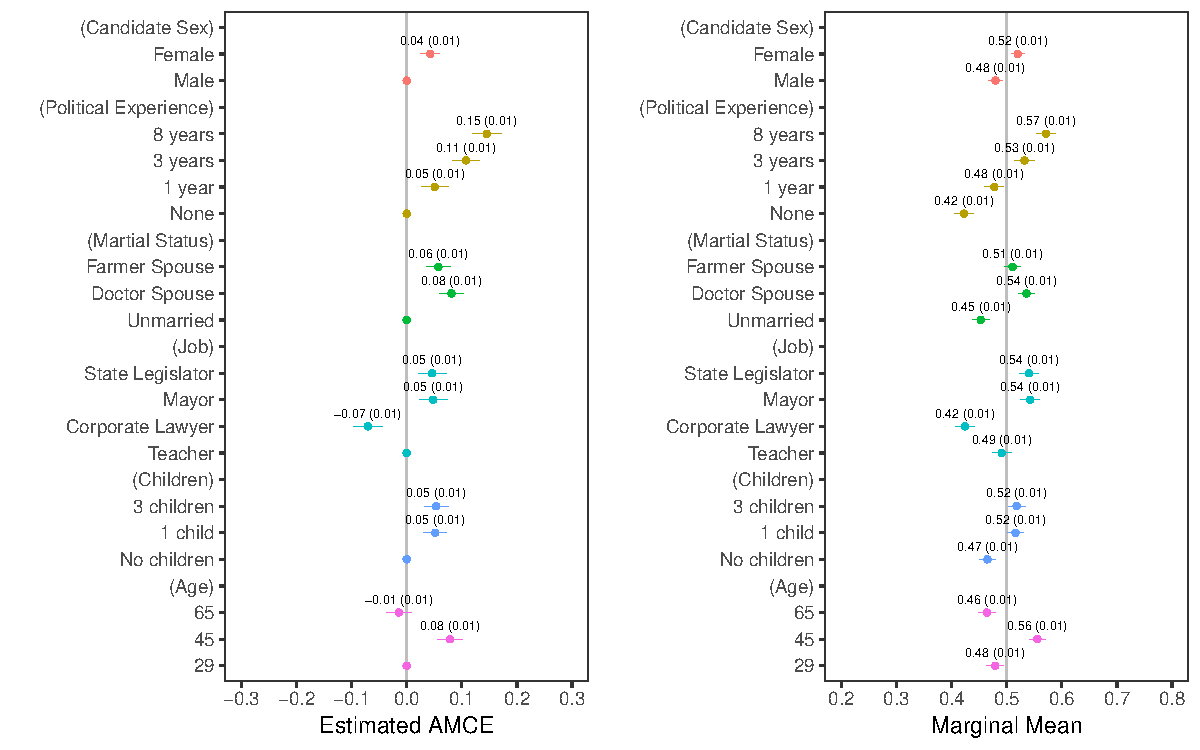
\includegraphics[width=\maxwidth]{figure/tkr_amce_appendix-1} 

\end{knitrout}

\clearpage

% latex table generated in R 3.5.1 by xtable 1.8-3 package
% Sun Nov 25 10:43:16 2018
\begin{table}[ht]
\centering
\begin{tabular}{lp{1.5in}rrr}
  \hline
feature & level & estimate & std.error & z \\ 
  \hline
Candidate Sex & Male & 0.00 &  &  \\ 
  Candidate Sex & Female & 0.04 & 0.01 & 4.74 \\ 
  Political Experience & None & 0.00 &  &  \\ 
  Political Experience & 1 year & 0.05 & 0.01 & 4.06 \\ 
  Political Experience & 3 years & 0.11 & 0.01 & 8.47 \\ 
  Political Experience & 8 years & 0.15 & 0.01 & 10.83 \\ 
  Martial Status & Unmarried & 0.00 &  &  \\ 
  Martial Status & Doctor Spouse & 0.08 & 0.01 & 7.25 \\ 
  Martial Status & Farmer Spouse & 0.06 & 0.01 & 5.26 \\ 
  Job & Teacher & 0.00 &  &  \\ 
  Job & Corporate Lawyer & -0.07 & 0.01 & -5.29 \\ 
  Job & Mayor & 0.05 & 0.01 & 3.74 \\ 
  Job & State Legislator & 0.05 & 0.01 & 3.59 \\ 
  Children & No children & 0.00 &  &  \\ 
  Children & 1 child & 0.05 & 0.01 & 4.84 \\ 
  Children & 3 children & 0.05 & 0.01 & 4.77 \\ 
  Age & 29 & 0.00 &  &  \\ 
  Age & 45 & 0.08 & 0.01 & 7.07 \\ 
  Age & 65 & -0.01 & 0.01 & -1.24 \\ 
   \hline
\end{tabular}
\end{table}


\clearpage

\subsection{Replication using MMs}

\begin{knitrout}
\definecolor{shadecolor}{rgb}{0.969, 0.969, 0.969}\color{fgcolor}
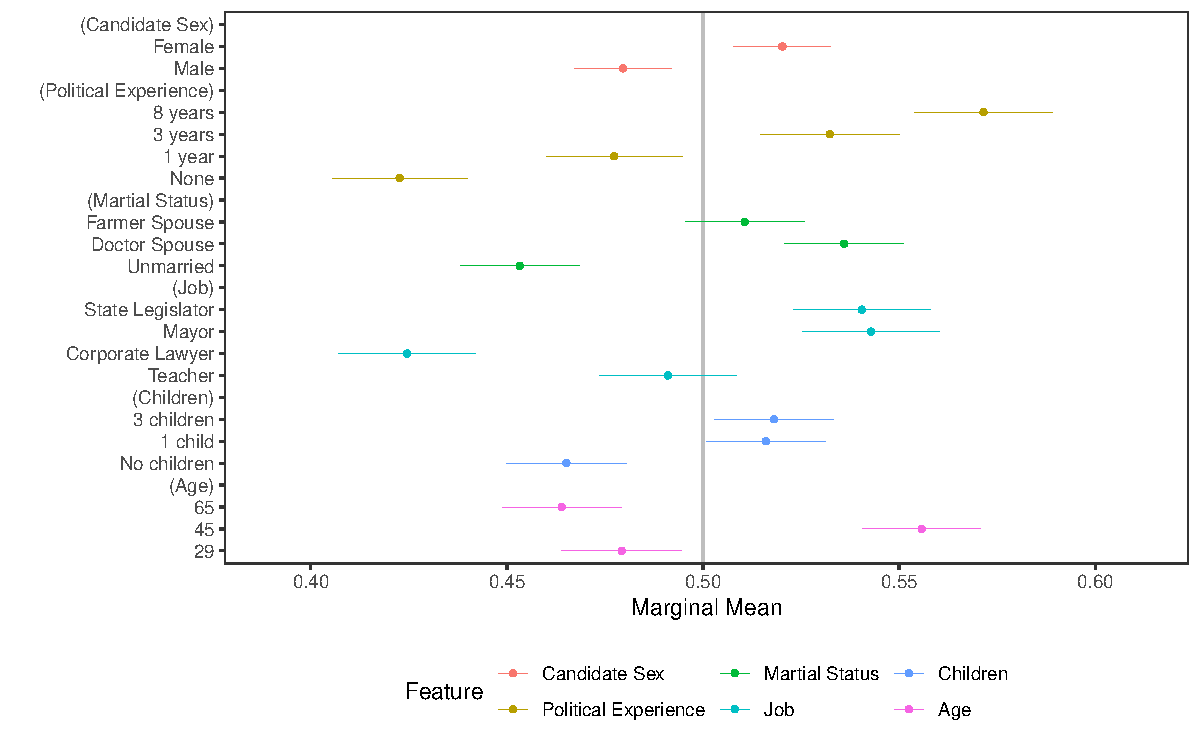
\includegraphics[width=\maxwidth]{figure/tkr_mm_appendix-1} 

\end{knitrout}

\clearpage

% latex table generated in R 3.5.1 by xtable 1.8-3 package
% Sun Nov 25 10:43:19 2018
\begin{table}[ht]
\centering
\begin{tabular}{lp{1.5in}rrr}
  \hline
feature & level & estimate & std.error & z \\ 
  \hline
Candidate Sex & Male & 0.48 & 0.01 & -3.22 \\ 
  Candidate Sex & Female & 0.52 & 0.01 & 3.20 \\ 
  Political Experience & None & 0.42 & 0.01 & -8.81 \\ 
  Political Experience & 1 year & 0.48 & 0.01 & -2.56 \\ 
  Political Experience & 3 years & 0.53 & 0.01 & 3.58 \\ 
  Political Experience & 8 years & 0.57 & 0.01 & 7.99 \\ 
  Martial Status & Unmarried & 0.45 & 0.01 & -6.05 \\ 
  Martial Status & Doctor Spouse & 0.54 & 0.01 & 4.66 \\ 
  Martial Status & Farmer Spouse & 0.51 & 0.01 & 1.37 \\ 
  Job & Teacher & 0.49 & 0.01 & -1.01 \\ 
  Job & Corporate Lawyer & 0.42 & 0.01 & -8.44 \\ 
  Job & Mayor & 0.54 & 0.01 & 4.77 \\ 
  Job & State Legislator & 0.54 & 0.01 & 4.55 \\ 
  Children & No children & 0.47 & 0.01 & -4.47 \\ 
  Children & 1 child & 0.52 & 0.01 & 2.07 \\ 
  Children & 3 children & 0.52 & 0.01 & 2.34 \\ 
  Age & 29 & 0.48 & 0.01 & -2.65 \\ 
  Age & 45 & 0.56 & 0.01 & 7.28 \\ 
  Age & 65 & 0.46 & 0.01 & -4.66 \\ 
   \hline
\end{tabular}
\end{table}


\clearpage

\subsection{Subgroup Analysis for Teele et al. (2018) Candidate Experiment using AMCEs}

\begin{knitrout}
\definecolor{shadecolor}{rgb}{0.969, 0.969, 0.969}\color{fgcolor}
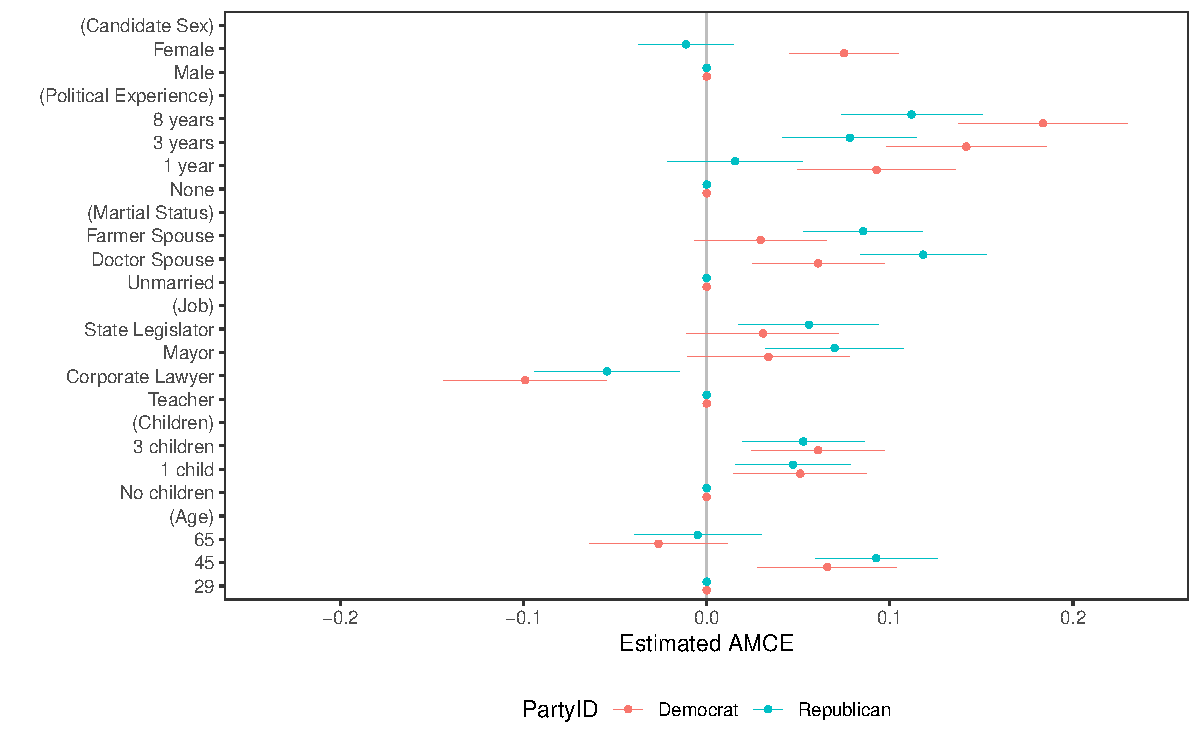
\includegraphics[width=\maxwidth]{figure/tkr_subgroup_amce_appendix-1} 

\end{knitrout}

\subsection{Subgroup Analysis for Teele et al. (2018) Candidate Experiment using MMs}

\begin{knitrout}
\definecolor{shadecolor}{rgb}{0.969, 0.969, 0.969}\color{fgcolor}
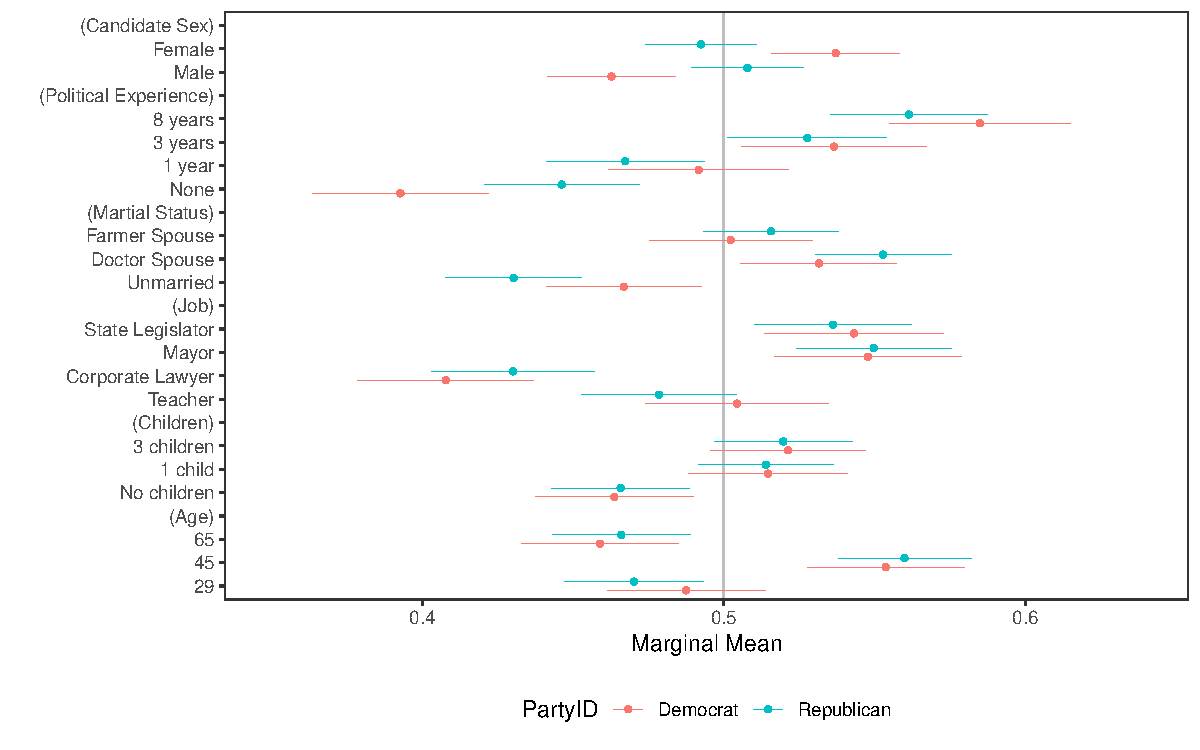
\includegraphics[width=\maxwidth]{figure/tkr_subgroup_mm_appendix-1} 

\end{knitrout}

\clearpage

\subsection{Comparison of Alternative Reference Categories for Teele et al. (2018) Candidate Experiment}




\begin{knitrout}
\definecolor{shadecolor}{rgb}{0.969, 0.969, 0.969}\color{fgcolor}
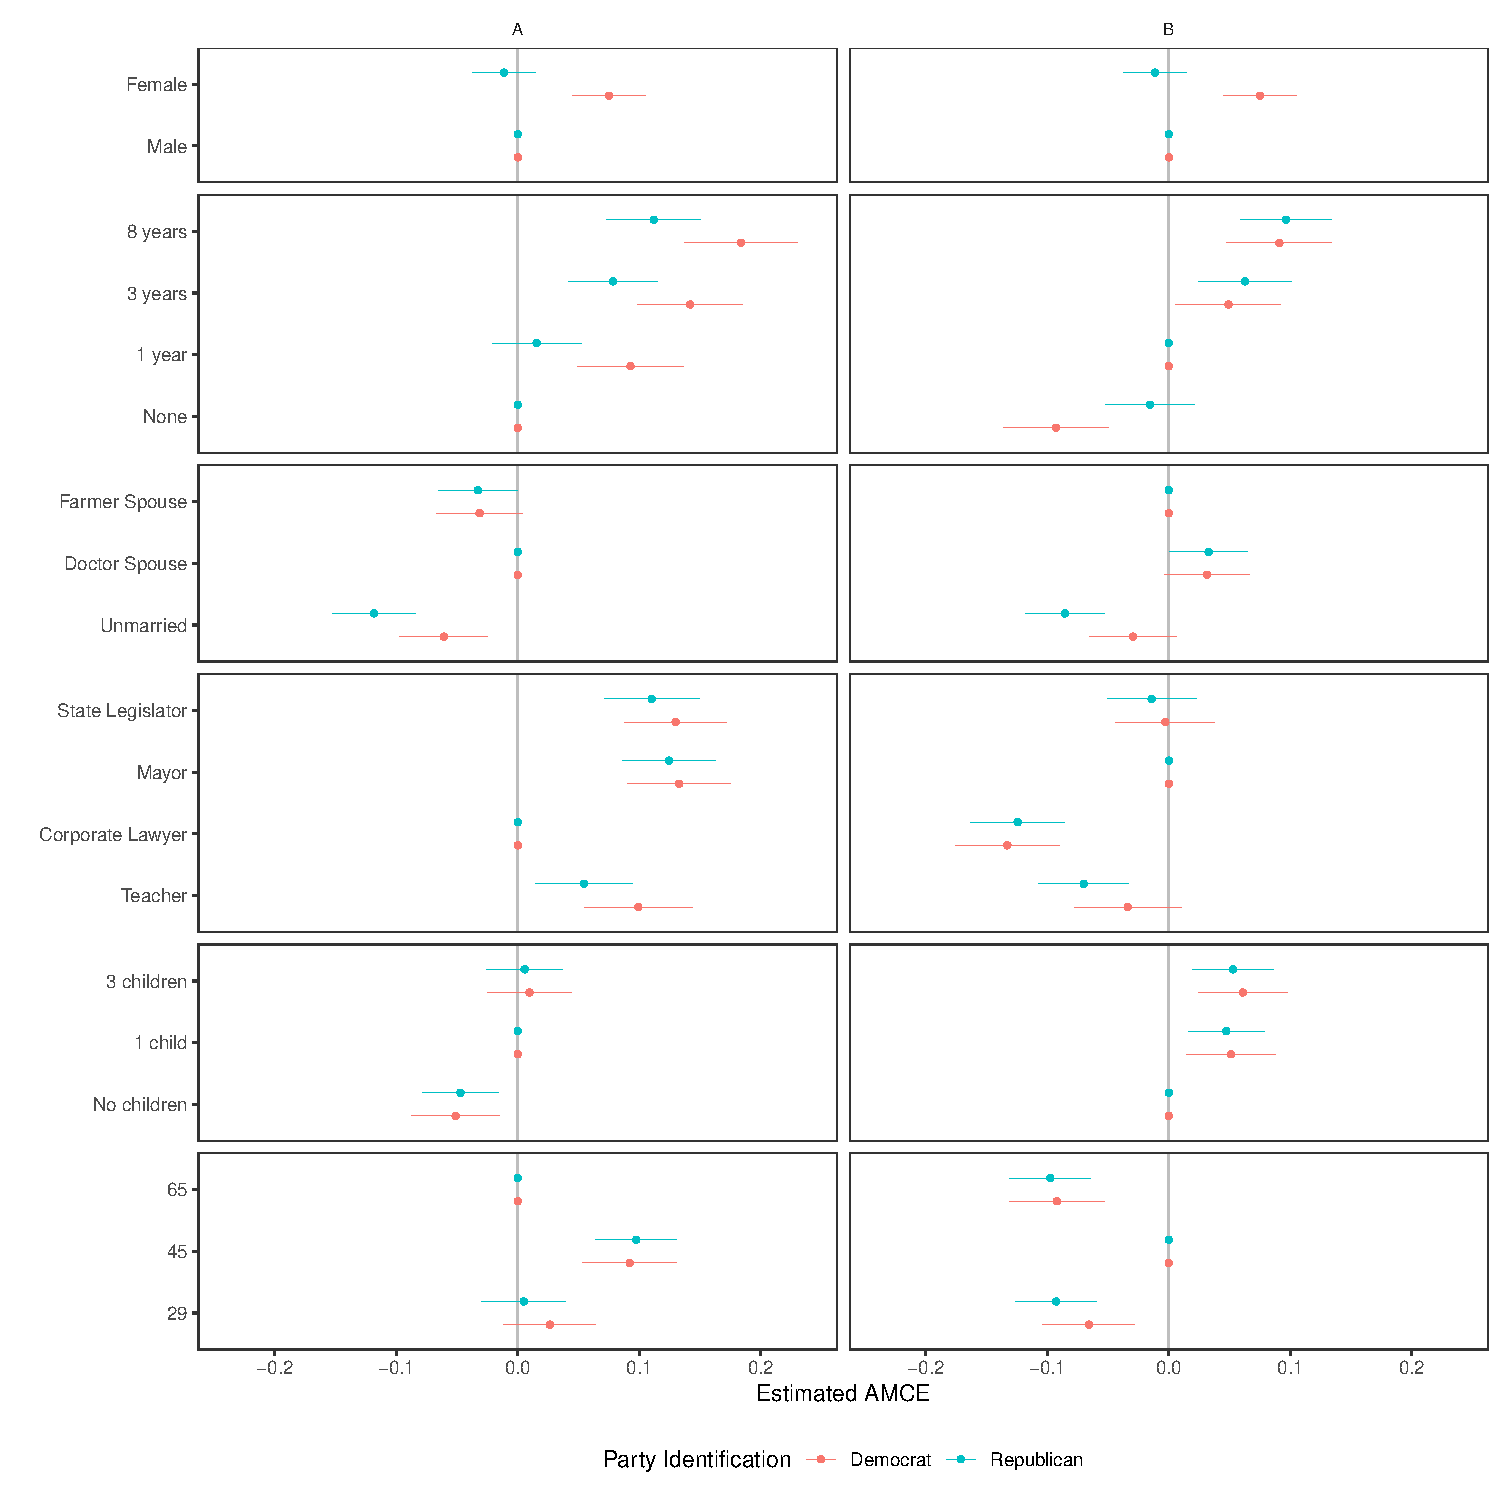
\includegraphics[width=\maxwidth]{figure/tkr_subgroup_example_plot-1} 

\end{knitrout}


\clearpage

\section*{}

\noindent This paper was built using \texttt{knitr::knit2pdf()} under the following environment:

\begin{knitrout}
\definecolor{shadecolor}{rgb}{0.969, 0.969, 0.969}\color{fgcolor}\begin{kframe}
\begin{verbatim}
## R version 3.5.1 (2018-07-02)
## Platform: x86_64-w64-mingw32/x64 (64-bit)
## Running under: Windows 7 x64 (build 7601) Service Pack 1
## 
## Matrix products: default
## 
## locale:
## [1] LC_COLLATE=English_United Kingdom.1252 
## [2] LC_CTYPE=English_United Kingdom.1252   
## [3] LC_MONETARY=English_United Kingdom.1252
## [4] LC_NUMERIC=C                           
## [5] LC_TIME=English_United Kingdom.1252    
## 
## attached base packages:
## [1] stats     graphics  grDevices utils     datasets  methods   base     
## 
## other attached packages:
## [1] ggplot2_3.1.0 cregg_0.3.0   rio_0.5.16   
## 
## loaded via a namespace (and not attached):
##  [1] zip_1.0.0         Rcpp_1.0.0        cellranger_1.1.0 
##  [4] pillar_1.3.0.9000 compiler_3.5.1    plyr_1.8.4       
##  [7] bindr_0.1.1       forcats_0.3.0     tools_3.5.1      
## [10] digest_0.6.18     lattice_0.20-38   ggstance_0.3.1   
## [13] evaluate_0.12     tibble_1.4.2      gtable_0.2.0     
## [16] pkgconfig_2.0.2   rlang_0.3.0.1     Matrix_1.2-15    
## [19] openxlsx_4.1.0    curl_3.2          haven_2.0.0      
## [22] bindrcpp_0.2.2    withr_2.1.2       stringr_1.3.1    
## [25] dplyr_0.7.8       knitr_1.20        hms_0.4.2        
## [28] lmtest_0.9-36     tidyselect_0.2.5  grid_3.5.1       
## [31] glue_1.3.0        data.table_1.11.8 R6_2.3.0         
## [34] survival_2.43-3   readxl_1.1.0      foreign_0.8-71   
## [37] purrr_0.2.5       magrittr_1.5      splines_3.5.1    
## [40] scales_1.0.0      assertthat_0.2.0  xtable_1.8-3     
## [43] colorspace_1.3-2  sandwich_2.5-0    survey_3.34      
## [46] stringi_1.2.4     lazyeval_0.2.1    munsell_0.5.0    
## [49] crayon_1.3.4      zoo_1.8-4
\end{verbatim}
\end{kframe}
\end{knitrout}

\end{document}
